
\documentclass[12pt]{report}

%--------------- libs requires to display one image over two pages ------------------%

\usepackage{graphicx}
\usepackage{adjustbox}
\usepackage{afterpage}
\usepackage{placeins}


% For the `memoir` class remove the following two packages.
% This class already provide the functionality of both
\usepackage{caption}
\usepackage[strict]{changepage}
%%%

\setcounter{totalnumber}{1}
\setcounter{topnumber}{1}
\setcounter{bottomnumber}{1}
\renewcommand{\topfraction}{.99}
\renewcommand{\bottomfraction}{.99}
\renewcommand{\textfraction}{.01}

\usepackage{graphicx}
\usepackage{geometry}
\usepackage[strict]{changepage}
\usepackage{afterpage,adjustbox}
\usepackage{caption}

\makeatletter
\newcommand{\twopagepicture}[4]{%
	{\afterpage{%
			\begin{figure}[#1]
				\caption{#4}%
				\makebox[\textwidth][l]{%
					\let\mywidth\linewidth
					\adjustbox{trim=0 0 {.5\width} 0,clip}{\includegraphics[width=2\mywidth]{#3}}}%
				\caption*{.}%
			\end{figure}%
			\begin{figure}[#1]
				\caption*{\phantom{#4}}%
				\makebox[\textwidth][l]{%
					\let\mywidth\linewidth
					\adjustbox{trim={.5\width} 0 0 0,clip}{\includegraphics[width=2\mywidth]{#3}}}%
			\end{figure}%
	}}%
}
\makeatother
%-------------------------------------------------%

% margin left and right with \setlength{\itemindent}{-.5in} %
\usepackage{enumitem}

% leave out section numbers in subsection numbering %
\usepackage[T1]{fontenc}
\renewcommand*\thesubsection{\arabic{subsection}}

% include Roman numerals for sections %
\renewcommand{\thesection}{\Roman{section}}
%Roman numerals for subsections like this \renewcommand{\thesubsection}{\Roman{subsection}}%
% include the package of the color%
\usepackage[usenames, dvipsnames]{color}
\usepackage[english]{babel}
\usepackage[utf8x]{inputenc}
\usepackage{amsmath}
\usepackage{graphicx}
\usepackage{subfiles}

\newcommand*{\captionsource}[2]{%
	\caption[{#1}]{%
		#1%
		\\\hspace{\linewidth}%
		\textbf{source:} #2%
	}%
}

%define your own color %
\definecolor{mygray}{gray}{0.9}
\begin{document}
	\tableofcontents{}
	\listoffigures
	\listoftables
		% include chapter 1 %
      \clearpage
      \newpage
      \documentclass[12pt]{article}

% leave out section numbers in subsection numbering %
\usepackage[T1]{fontenc}
\renewcommand*\thesubsection{\arabic{subsection}}

% include Roman numerals for sections %
\renewcommand{\thesection}{\Roman{section}}
%Roman numerals for subsections like this \renewcommand{\thesubsection}{\Roman{subsection}}%
% include the package of the color%
\usepackage[usenames, dvipsnames]{color}
\usepackage[english]{babel}
\usepackage[utf8x]{inputenc}
\usepackage{amsmath}
\usepackage{graphicx}
\usepackage{subfiles}

%define your own color %
\definecolor{mygray}{gray}{0.9}
\begin{document}
	\listoffigures
	\title{Chapter 1 : General Project Presentation}
	\maketitle

	\section{Host Company Presentation}
	
	\subsection{Presentation of MASS Analytics}
	MASS Analytics, a Tunisian start-up founded in 2012, is the first and only independent Marketing Mix Modeling (MMM) agency in the MENA region. MASS Analytics’ core competency is the deep analysis and understanding of what impacts the consumer's path to purchase to make companies more effective with their marketing budget.
	\\
	\\
	It was founded by \textbf{Dr. Ramla Jarrar } ( Chief Executive Officer ),  \textbf{Dr. Firas Jabloun } (Chief Technology Officer), \textbf{Nadia Bouzguenda} (Business Development Director) \& \textbf{Rafal Kozlowski} (Director). They brought the essence of more than 20 cumulative years of experience in marketing effectiveness \& technology services at the international level to the creation of MASS-Analytics. \cite{ref1}
	\\
	\\
	\begin{figure}[h]
	\centering
	
\includegraphics[width=0.15\textwidth]{Mass_logo.png}
	\caption{Mass-Analytics logo}
    \end{figure}
	\subsection{Services}
	\begin{itemize}
		\item \textbf{MassTer Software :} MASS Analytics has been developing internally its own Marketing Mix Modeling Software ``MassTer''. It is one of the most powerful Marketing Mix Modeling software products/solutions in the world and comes in three packages: standard, professional , and premium. It provides the user with a powerful Modeling platform coupled with a comprehensive data visualization capability to help understand the relationship between different variables and measure their impact on business performance.
			\begin{figure}[h]
			\centering
			
\includegraphics[width=0.2\textwidth]{massTer_logo.png}
			\caption{MassTer Software logo}
		\end{figure}
		
		\item \textbf{Training and Consultancy :} MASS Analytics runs specific courses and training sessions on advanced predictive modeling (log linear, nested modeling, fixed effect modeling…), budget optimization and return on Investment calculation. It also offers its clients coaching sessions to help improve their marketing analytics process and project delivery.
	\end{itemize}
\vspace{66mm}
	\subsection{Customers}
	
		\begin{figure}[h]
		\centering
		
\includegraphics[width=0.8\textwidth]{customers_logo.png}
		\caption{Some of MASS Analytics’ customers logo}
	\end{figure}
	\section{Project Presentation}
	
	\subsection{Context}
	As part of its software development and consulting activities, oriented towards the business of Marketing Mix Modelling (MMM), Mass-Analytics is always looking to offer its customers products that are the most efficient and smart. Thus, It seeking to provide innovative services that satisfied the different needs of customers based on new technologies.
	\\
	\\
	In this context, this project entitled \textbf{MassTer Insight SaaS} was offered to me by Mass-Analytics as part of a graduation project to obtain the national diploma of computer engineer.      
	\subsection{Objectives}
	The main objectif of this project is to develop MassTer Insight from the exiting Desktop solution to a SaaS.
	\\
	\\
	We are in charge to keep the same business logic of the desktop solution, but offered to the customers in cloud SaaS version with Security guaranteed,  high perform in term of Speed, Visualization, Graphics, Design .
	\subsection{Problematic}
	subSection for the Problematic ....

	\section{Life cycle}
	\section{Methodology}
	The choice of the methodology is an important step in software development since it grants formalizing the preliminary steps when establishing a system in pursuance of the client’s requirements.
	The  ? scrum ? TDD, an approach that is part of the Agile movement, was used when carrying out this project.
		\section{Existing Presentation}
	\textbf{MassTer Insight Desktop Application} is an easy to use software that allows you to run simulation scenarios and allocate your budget optimally across Regions, Products, Channels and Periods. It tells you how much budget to spend on every single media channel and in which period, given a complex modelling structure. It will helps you to benefit from your Marketing Mix Modelling projects [1]. 
	\section{Critics}
	Today all the company move to cloud, they are tend to by their softwares through cloud SaaS, for more reasons : one amongst the reason is the security, when you offer an excutable software, this one is threaten by the crack, also an excutable requieres sometimes to take care of your resources needs, an important RAM, CPU, and more. Almost the Exutable save data locally which is a very bad way to stock data, it is possible to loose these data once the hard disk is defect by an external effect or even internal.
	\\
	\\
	That's what we care about, our current solution Masster Insight desktop is threateen by the crack, may will be heavy on machine with smaller resources, works only on pc. it requires the process of installation wasted time.
	  
	\section{Conclusion}
	This chapter was a presentation of the hosting company, its services, and clients. The problematic of the project was also highlighted, along with the proposed solution and the methodology followed while carrying out the project.
	\bibliographystyle{plain}
	\bibliography{webo} 
\end{document}
	
	
		% include chapter 2 %
   	\clearpage
	\newpage
	
\documentclass[12pt]{article}

% margin left and right with \setlength{\itemindent}{-.5in} %
\usepackage{enumitem}

% leave out section numbers in subsection numbering %
\usepackage[T1]{fontenc}
\renewcommand*\thesubsection{\arabic{subsection}}


% include Roman numerals for sections %
\renewcommand{\thesection}{\Roman{section}}
%Roman numerals for subsections like this \renewcommand{\thesubsection}{\Roman{subsection}}%
% include the package of the color%
\usepackage[usenames, dvipsnames]{color}
\usepackage[english]{babel}
\usepackage[utf8x]{inputenc}
\usepackage{amsmath}
\usepackage{graphicx}
\usepackage{subfiles}

%define your own color %
\definecolor{mygray}{gray}{0.9}
\begin{document}
	\listoffigures
	\title{Chapter 2 : Analysis and specification of requirements}
	\maketitle
	
	\section{Introduction}
	Being the first in the development cycle of the project, this phase is the most
	important. Indeed, it is during this period that the needs of the user are identified and specified. These requirements also represent the functionalities that should be present in the application, which also makes it possible to validate the application as the development progresses.
	\section{Actors Identification}
	\textbf{MassTer Insight web Application }was mainly designed to be used by \textbf{Data Analysts }in MMM agencies, which is the case of \textbf{MASS Analytics}, \textbf{Media Agencies }that have a MMM division, and \textbf{Advertisers }who have an in-house MMM team.
	
	\clearpage
	\newpage
	
	
	\section{Requirement Analysis}

	\subsection{Functional Requirements}
     
	These functional requirements express the expectations of different users for the product to be produced.
	\\
	\\
	In this part, we present the different functionalities and services that the application must ensure.
	
	CONNECT TO SERVER
	\begin{itemize}
		\setlength{\itemindent}{+.5in}
		\item \textbf{Connect To MassTer Server : } 
	\end{itemize}
	
	LOAD PROJECT
	\begin{itemize}
		\setlength{\itemindent}{+.5in}
     	\item \textbf{Load MassTer Insight Project : } 
    \end{itemize}	
 
 	MANAGE REPORT
 		\begin{itemize}
 			\setlength{\itemindent}{+.5in}
 			\item \textbf{Available Reports : } 
 			\item \textbf{Save a Report : }
 			\item \textbf{Remove a Report : }
 			\item \textbf{Load a Report : } 
 			\item \textbf{Available Channel : } 
 			\item \textbf{Seasonality Index Per Month : }
 			\item \textbf{Ignore Preset Laydown : }
 			\item \textbf{Budget Tolerance : }
 			\item \textbf{Revenue Tolerance : }
 			\item \textbf{Max Iteration  : }
 			\item \textbf{Max Iteration  : }
 			\item \textbf{Budget Range : }
 			\item \textbf{Total Budget : }
 			\item \textbf{Min Target : }
 			\item \textbf{Select Channel : }
 			\item \textbf{Max budget/Min Target/Set Budget per Channel : }
 	\end{itemize}
 
  	UPDATE
    \begin{itemize}
    	\setlength{\itemindent}{+.5in}
    	\item \textbf{Update a Report : }
   \end{itemize}

  	RUN
   \begin{itemize}
   	   \setlength{\itemindent}{+.5in}
 	   \item \textbf{Run new scenario : }
   \end{itemize}

    \clearpage
    \newpage

	\subsection{Non-Functional Requirements}
	\begin{itemize}
		\item \textbf{Ergonomics : }The application offers a user-friendly and easy-to-use interface without refer to particular knowledge.
		\item \textbf{Security : }
		\item \textbf{Modularity : }a code that is easy to maintain and simple to understand in order to ensure the scalability of application. 
	\end{itemize}
	\clearpage
	\newpage
	
	\section{Use Case Diagrams}
	\subsection{Global Use Case Diagram}
	\clearpage
	\newpage
	\begin{figure}[h]
		\centering
		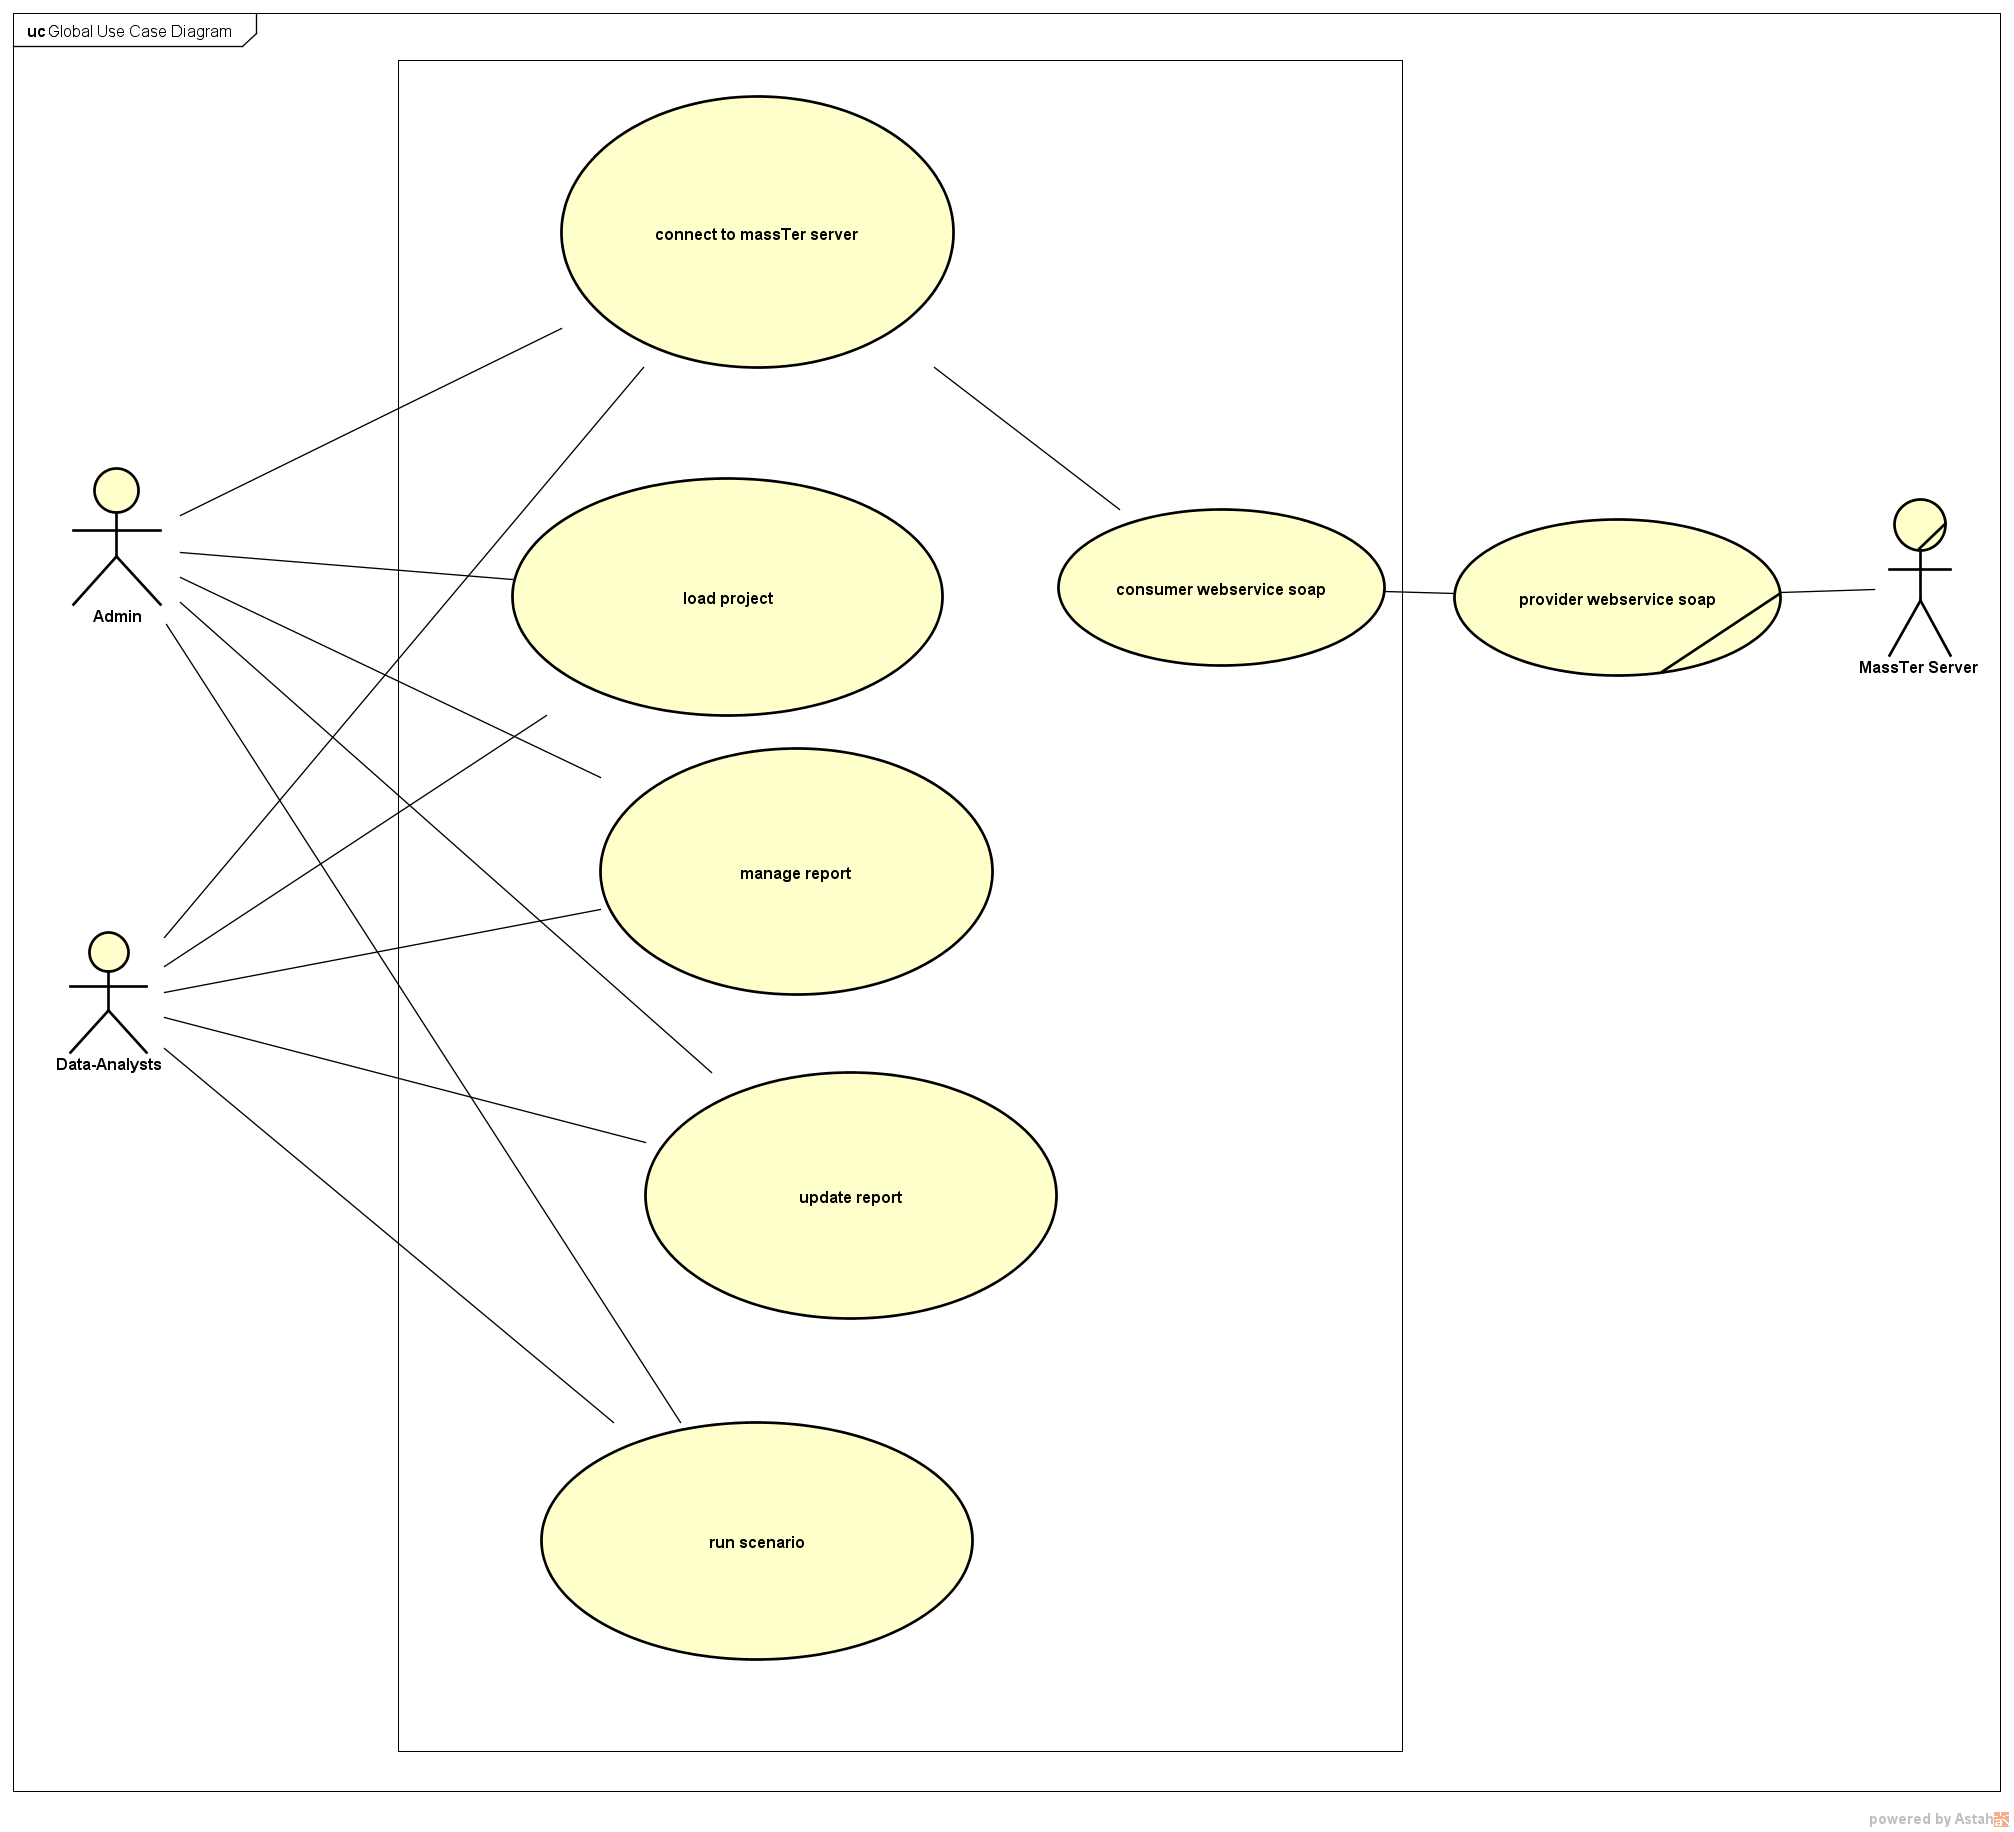
\includegraphics[width=1.0\textwidth]{GlobalUseCaseDiagram.png}
		\caption{Global Use Case Diagram}
		
	\end{figure}

\clearpage
\newpage


	\subsection{Detailed Use Case Diagrams}
	\clearpage
	\newpage
	 \subsubsection{connect to MassTer Server}
	 	\begin{figure}[h]
	 	\centering
	 	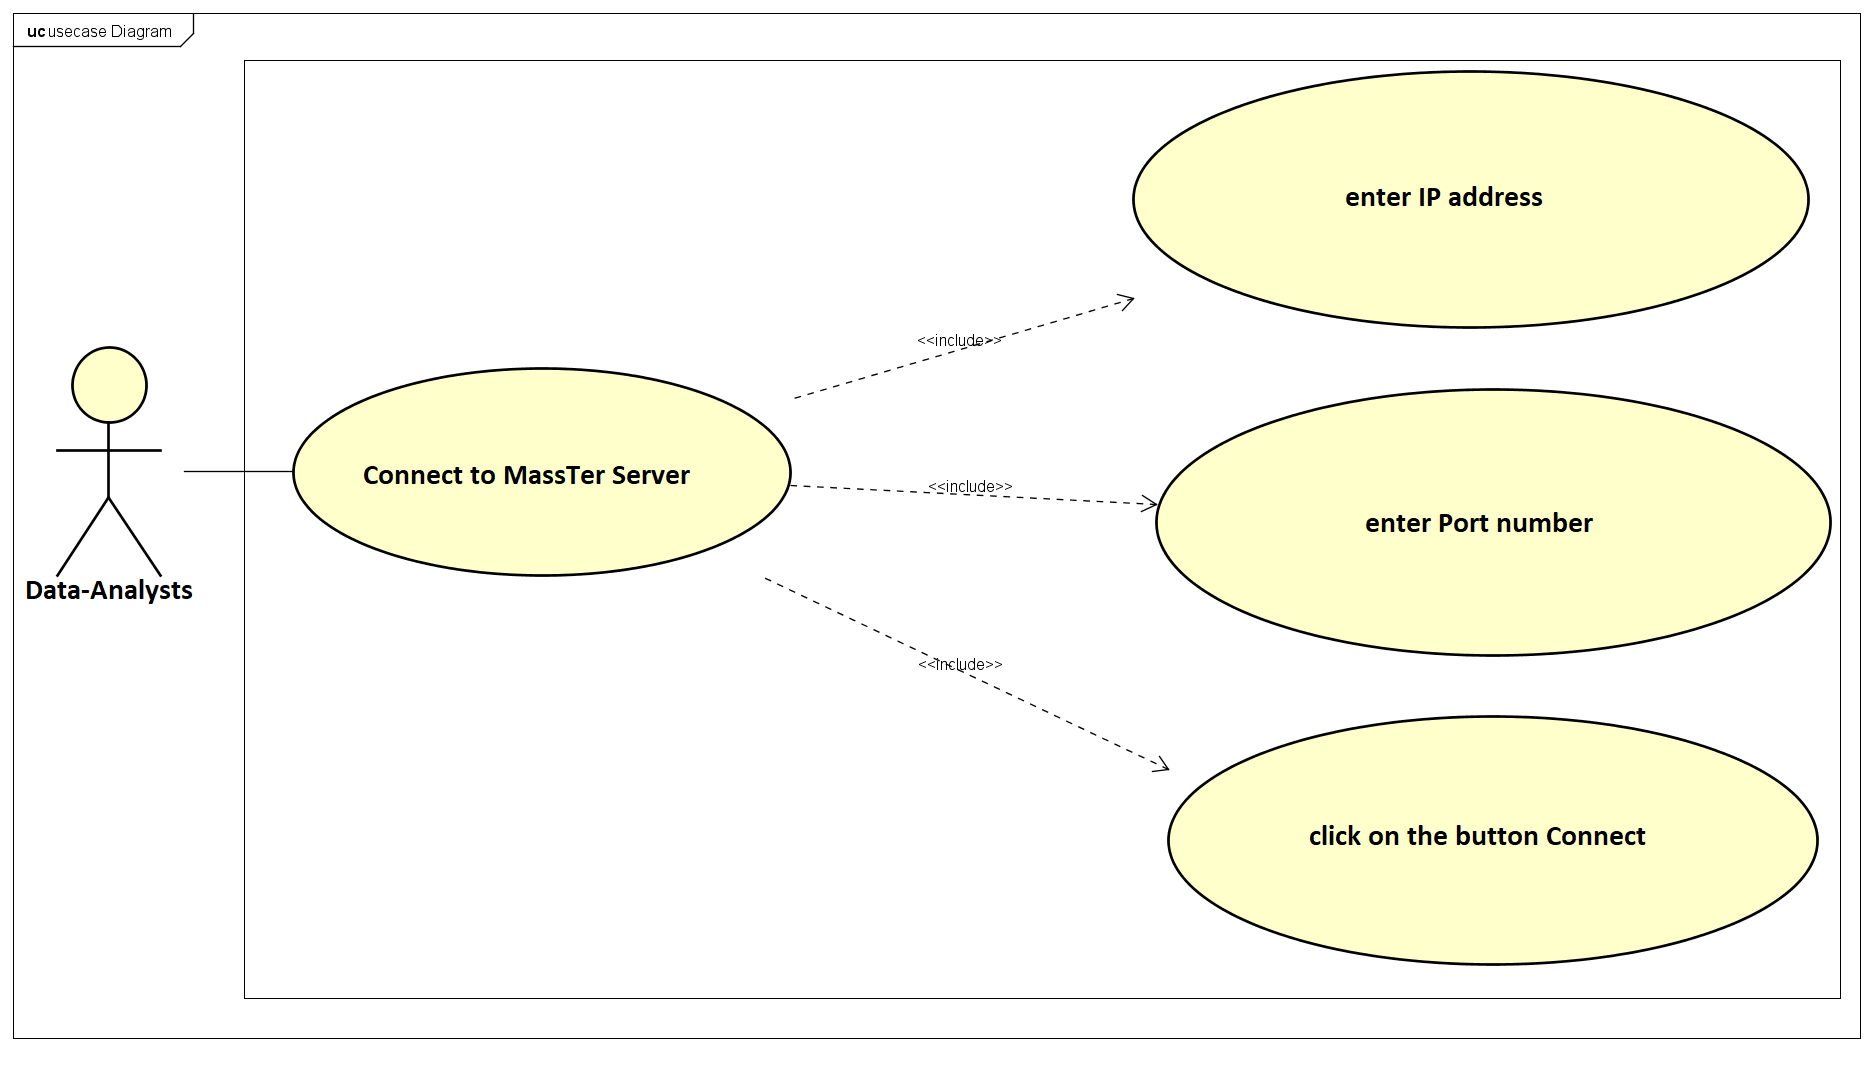
\includegraphics[width=1.0\textwidth]{connectToMassTerServer.png}
	 	\caption{connect to MassTer Server Use Case Diagram}
	 	
	 \end{figure}

  \newpage
 
 Description of the scenario ``connect to MassTer Server'' in the table below. 
 \\
 \begin{table}
 	\centering
 	\begin{tabular}{|c|p{10cm}|}
 		\hline
 		                        
 		\textbf{Nominal Scenario } & \\
 		\hline
 		....... & ... \\
 		
 		\hline
 	\end{tabular}
 \end{table}
 \clearpage
 \newpage
	 \subsubsection{consume webService soap}
	 	 	\begin{figure}[h]
	 	\centering
	 	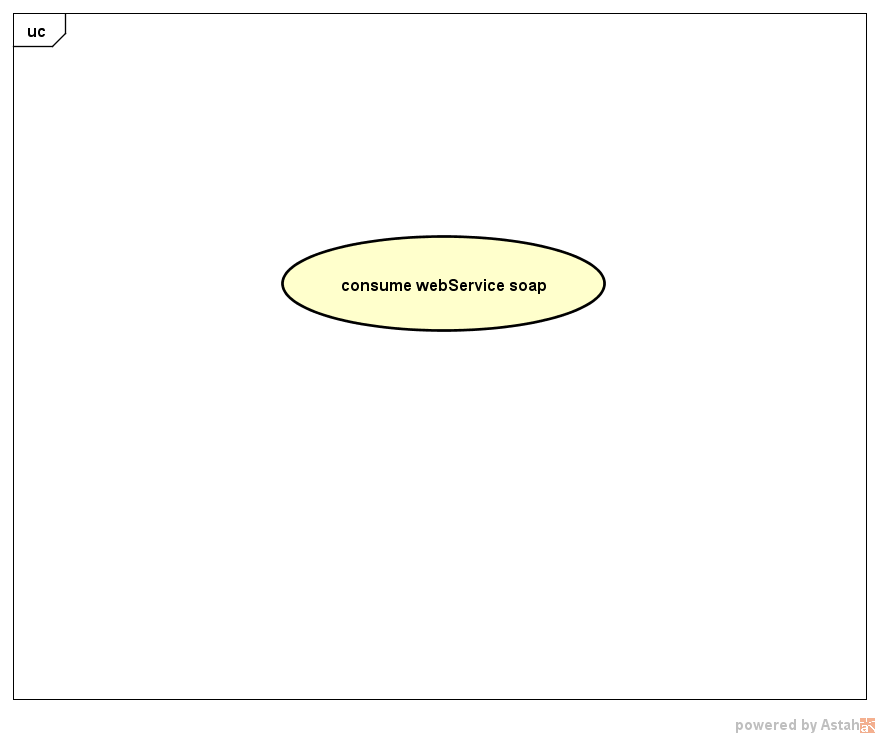
\includegraphics[width=1.0\textwidth]{consumewebServicesoap.png}
	 	\caption{consume webService soap Use Case Diagram}
	 	
	 \end{figure}
 Description of the scenario ``consume webService soap'' in the table below.
 \clearpage
 \newpage

	 \subsubsection{provide webService soap} 
	 	\begin{figure}[h]
	 	\centering
	 	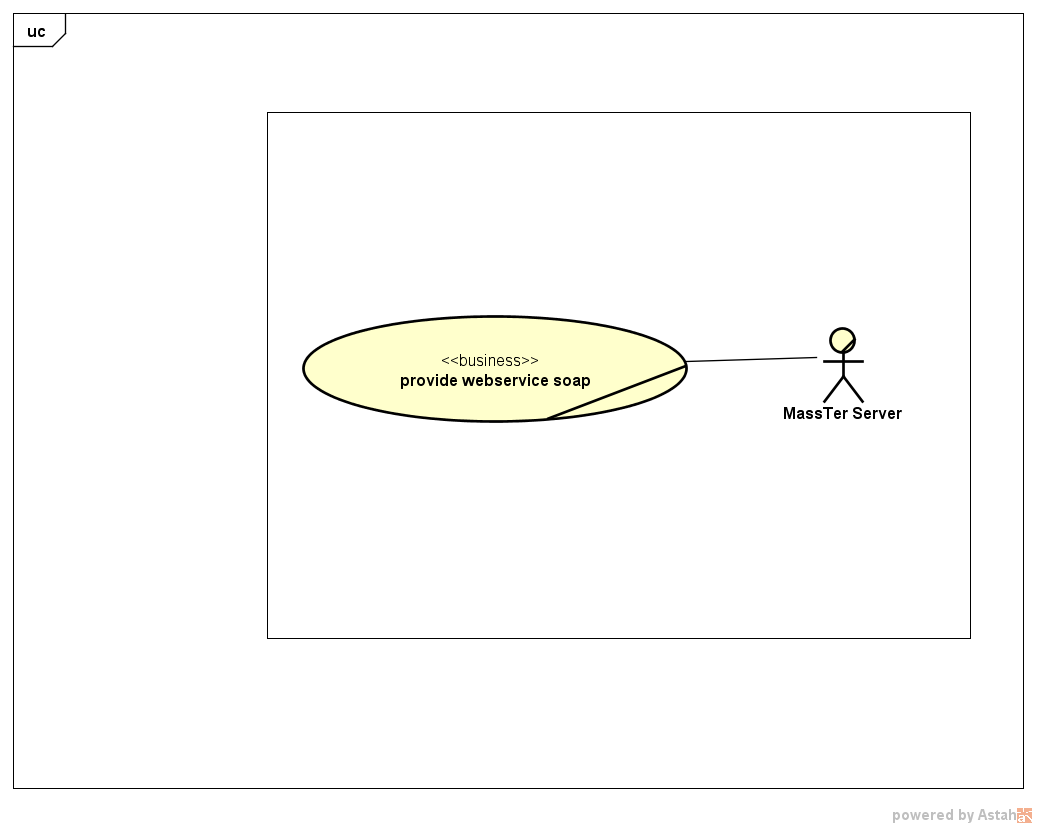
\includegraphics[width=1.0\textwidth]{provideWebServiceSoap.png}
	 	\caption{provide webService soap Use Case Diagram}
	 	
	 \end{figure}
  Description of the scenario ``consume webService soap'' in the table below.
 \clearpage
 \newpage
	 \subsubsection{load project}
	 	\begin{figure}[h]
	\centering
	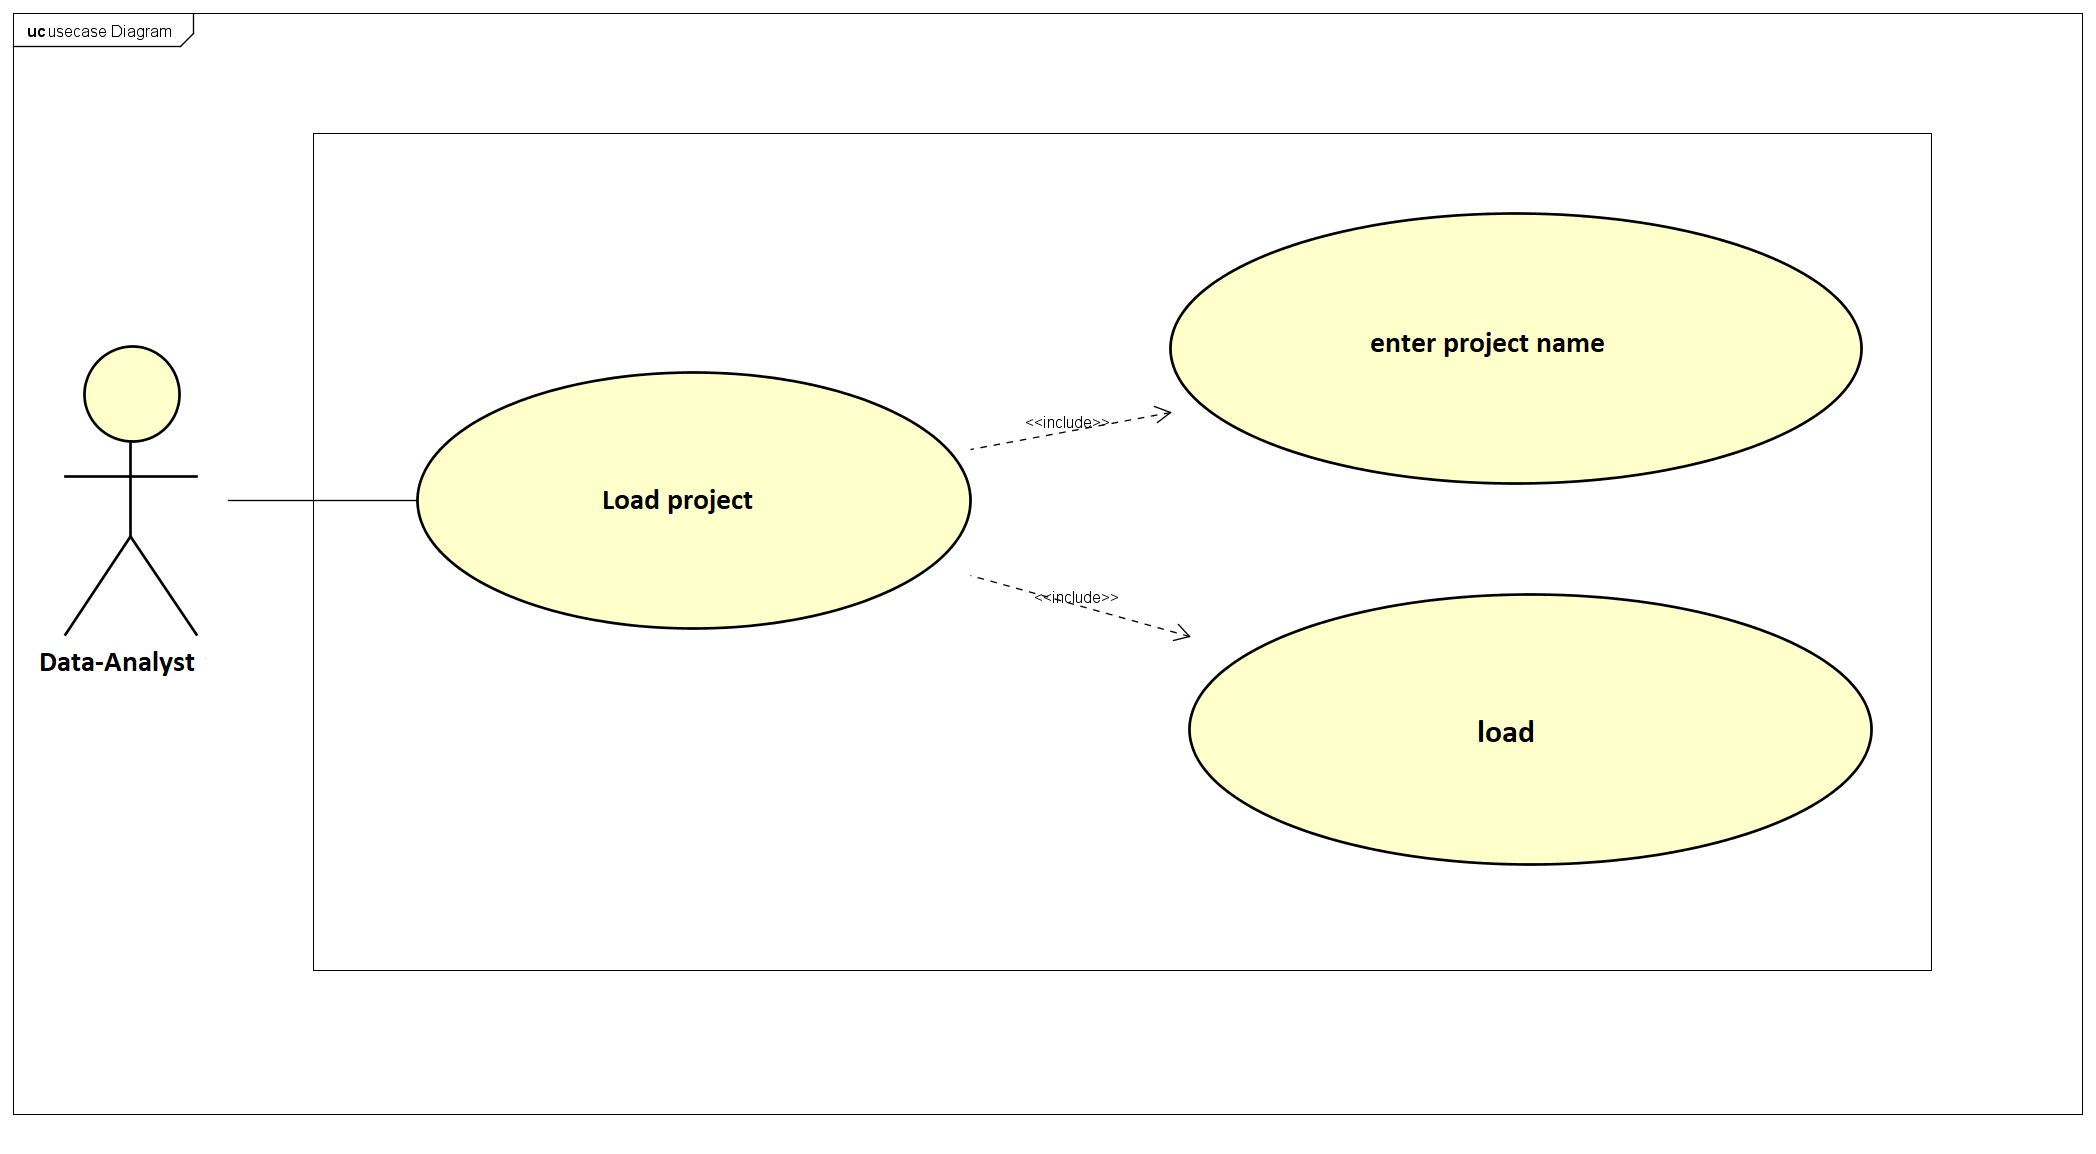
\includegraphics[width=1.0\textwidth]{loadProject.png}
	\caption{load project Use Case Diagram}
	
	\end{figure}
 Description of the scenario ``load project'' in the table below.
\clearpage
\newpage
	 \subsubsection{manage report}
	 	\begin{figure}[h]
	 	\centering
	 	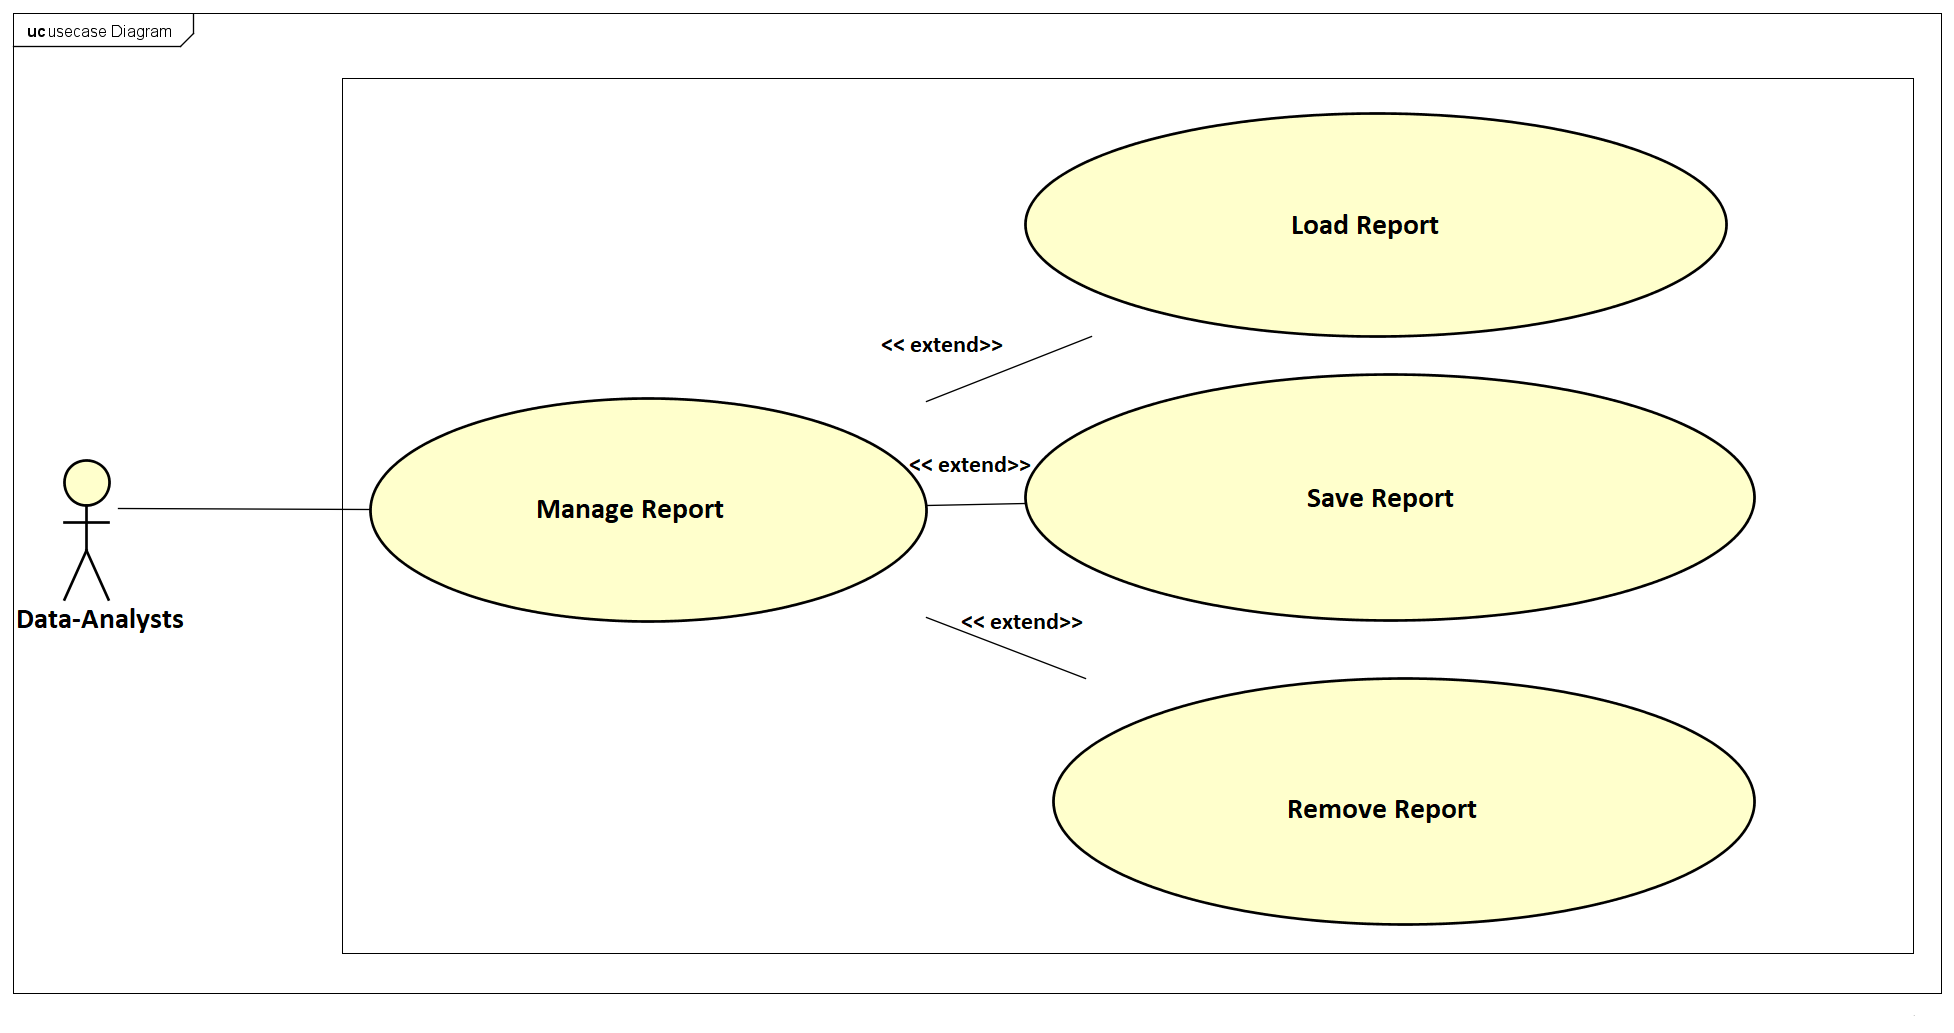
\includegraphics[width=1.0\textwidth]{manageReport.png}
	 	\caption{manage report Use Case Diagram}
	 	
	 \end{figure}
  Description of the scenario ``manage report'' in the table below.
 \clearpage
 \newpage
	 \subsubsection{update settings}
	 	\begin{figure}[h]
	 	\centering
	 	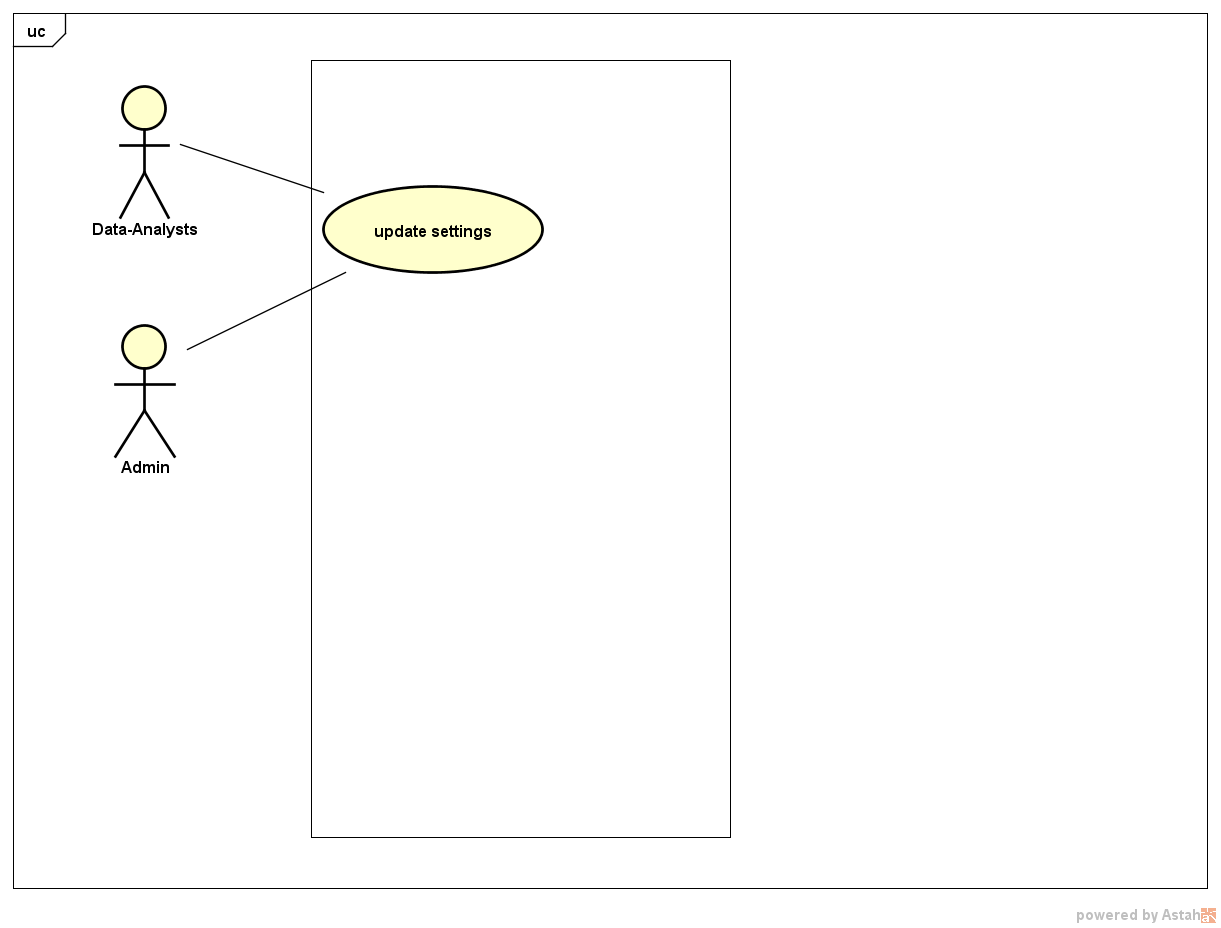
\includegraphics[width=1.0\textwidth]{updateSettings.png}
	 	\caption{update settings Use Case Diagram}
	 	
	 \end{figure}
  Description of the scenario ``update settings'' in the table below.
 \clearpage
 \newpage
	 \subsubsection{run scenario}
	 	\begin{figure}[h]
	 	\centering
	 	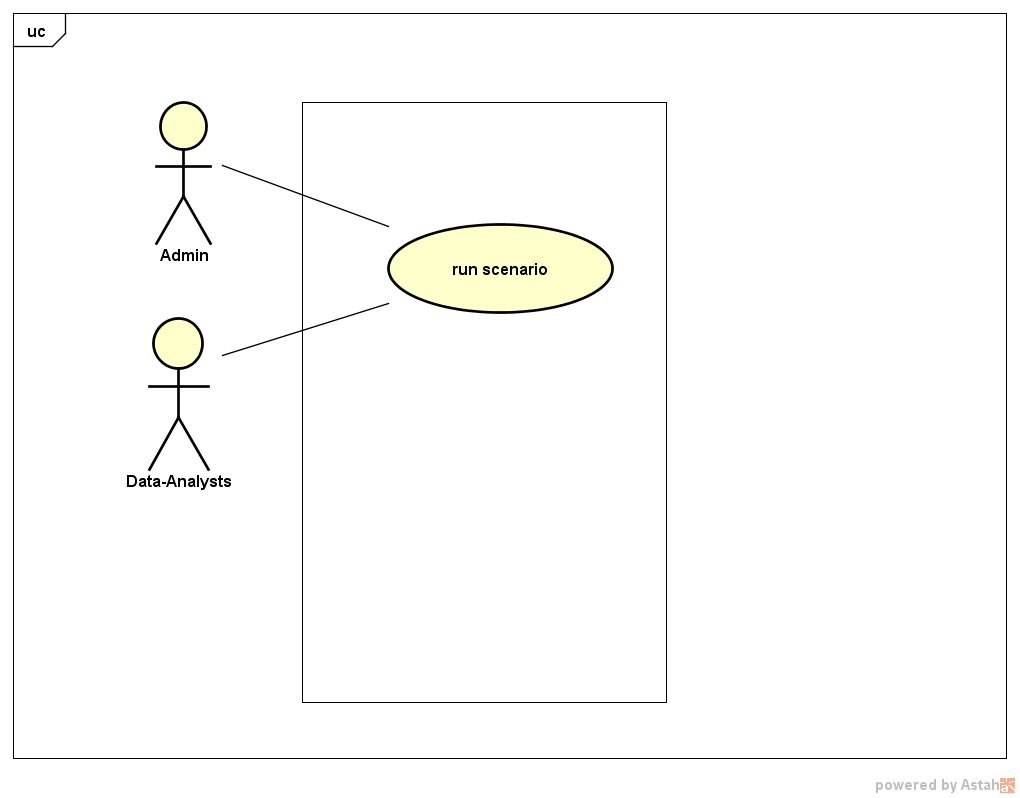
\includegraphics[width=1.0\textwidth]{runScenario.png}
	 	\caption{run scenario Use Case Diagram}
	 	
	 \end{figure}
	 Description of the scenario ``run scenario'' in the table below.
	
	\clearpage
	\newpage
	
	\section{Conclusion}
	
\end{document}
	
	% include chapter 3 %
	\clearpage
	\newpage
	
	\chapter{Conception}
	
	\section{Introduction}
	The aim of this chapter is  to study and design the features already determined in the previous phase of analysis and specification of requirements. For that, it is divided into two parts. The first part is dedicated to the exhibition of the choice of conception method as well as the architecture of the system to be developed. The second part presents the conception of the application with a set of diagrams.
	\section{Modeling Language}
		A modeling language is used to describe a system, a standard or methodology, general or domain-specific and / or context based on its components and relationships.
	There are several modeling languages, the best known are UML and Merise.
	\\
	\\
	In our project we chose UML as Modeling language, for two main reasons: 
	\begin{itemize}
	\item To obtain a very high level modeling independent of the language and environments
	\item Document a project. 
	\end{itemize}
	
	\section{Global Conception}
	In this section, we highlight the architecture of our application, we starting  with physical architecture and the logical architecture.
	
	\clearpage
	\newpage
	\subsection{Physical Architecture}
	It is primordial to designing any computer system to choose the model architecture that will be adequate to ensure proper functioning, performance, the reuse and reliable interconnection of this system with others. We opt for this purpose for the physical architecture described in the figure below.
	\begin{figure}[h]
		\centering
		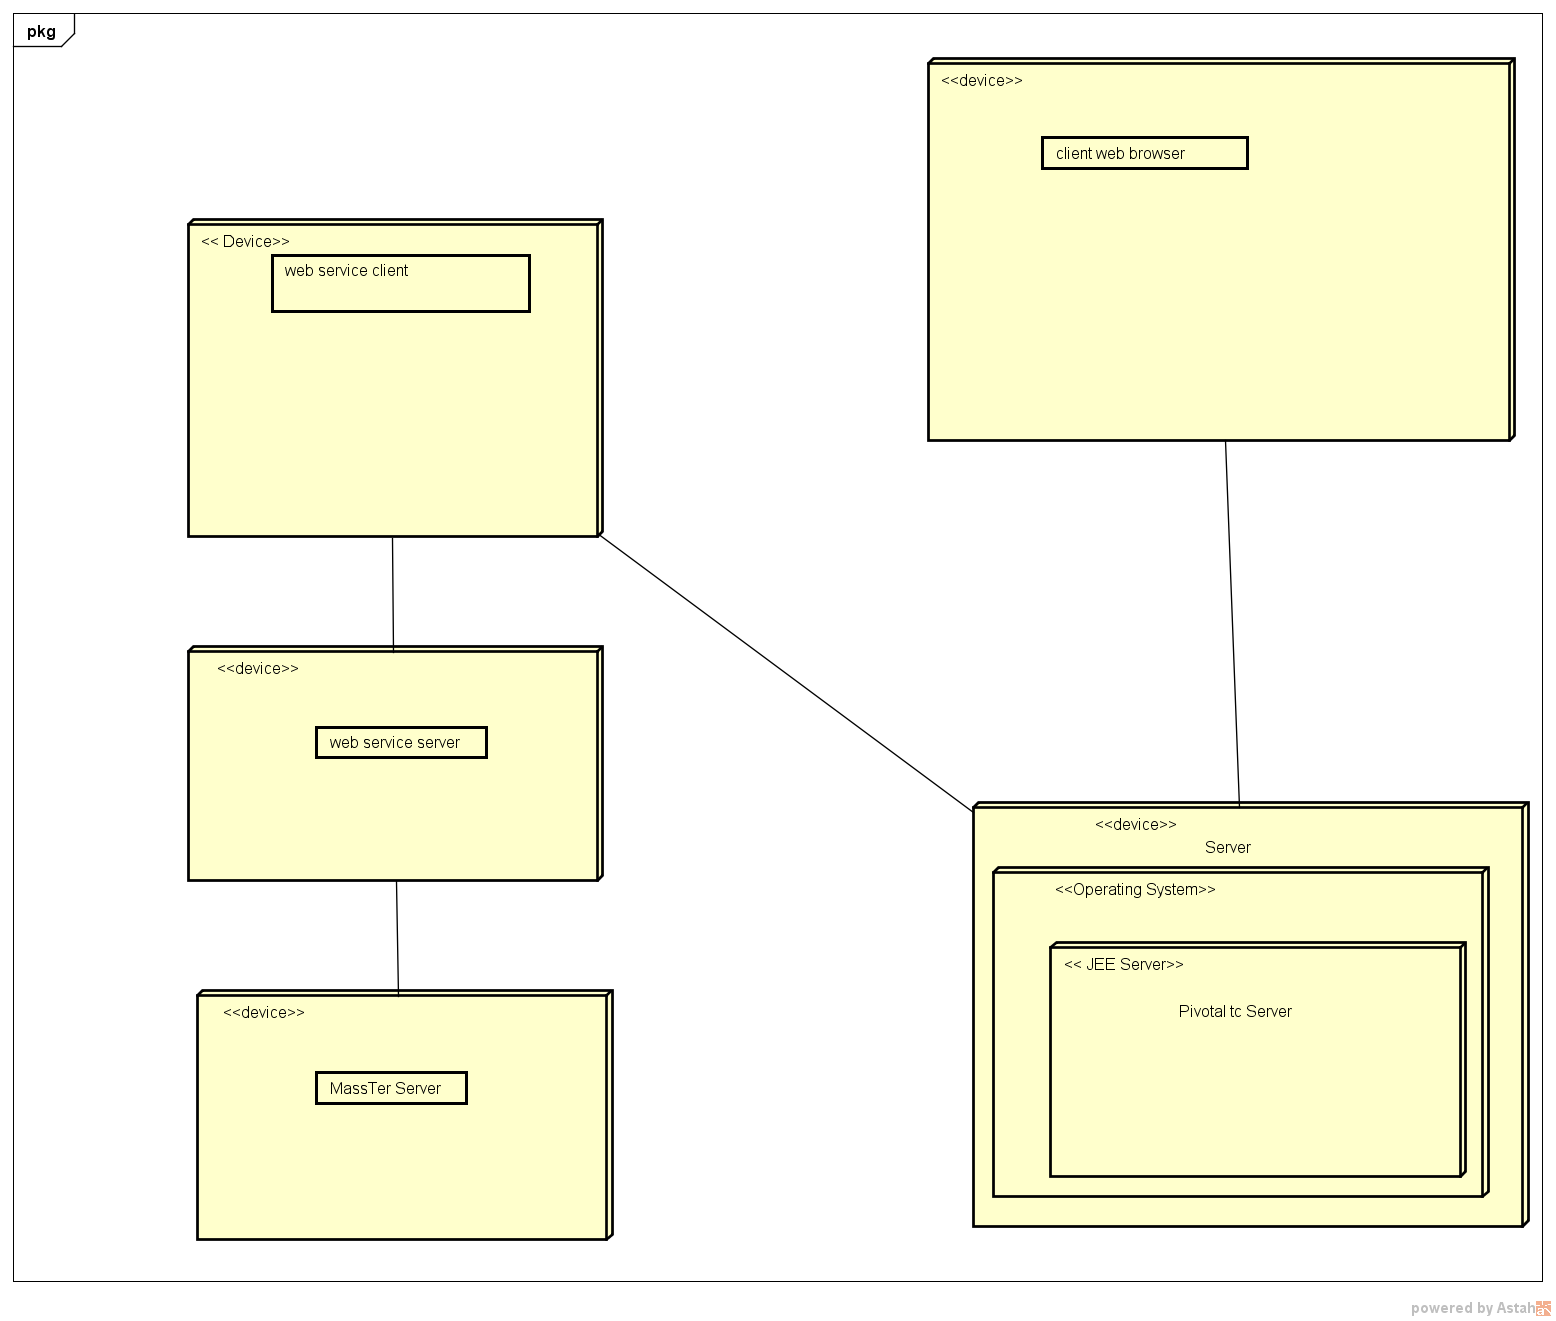
\includegraphics[width=16.5cm,height=12cm]{DeploymentDiagramPhysicalArchitecture.png}
		\caption{Deployment Diagram Physical Architecture}
	\end{figure}  

	\clearpage
    \newpage  
	
	\subsection{Logical Architecture}
 Fig. \ref{logicalArchitecture}	depicts the logical architecture in which different components interact.
\begin{figure}[h]
	\centering
	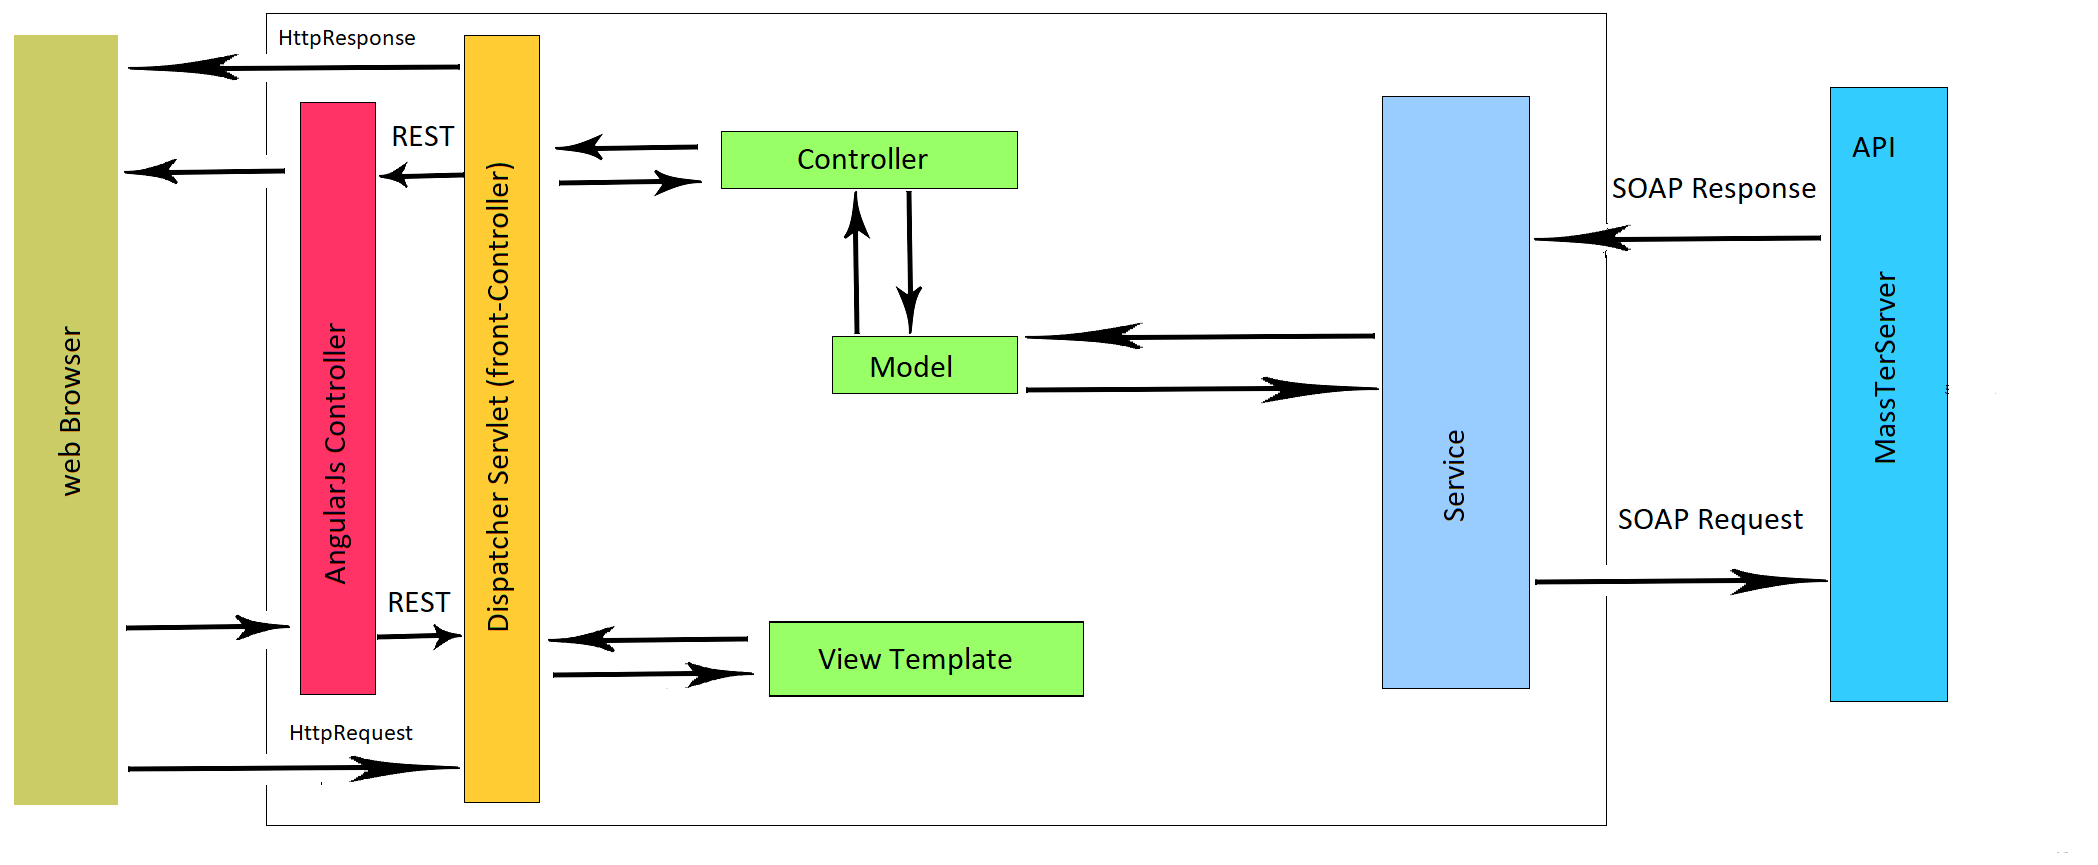
\includegraphics[width=17.5cm,height=9cm]{logicalArchitecture.png}
	\caption{Logical Architecture}
	\label{logicalArchitecture}
\end{figure} 
	
	\subsection{Design Pattern}
		We opt to use the MVC design pattern for the following benefits:
	\begin{itemize}
		\item \textbf{Reliability : }The presentation and business layers are completely separate, so that the business can change without necessarily affecting the presentation, or vice versa.
		\item \textbf{Adaptability : }Any visual representation can be easily integrated.
		\item \textbf{Productivity : }The duration of development is significantly reduced, in allowing parallel work teams.
		\item \textbf{Extensible : } With MVC the code is extensible.
	\end{itemize}

	\clearpage
    \newpage

	\section{Detailed Conception}
	\subsection{Package Diagram}
		\begin{figure}[h]
		\centering
		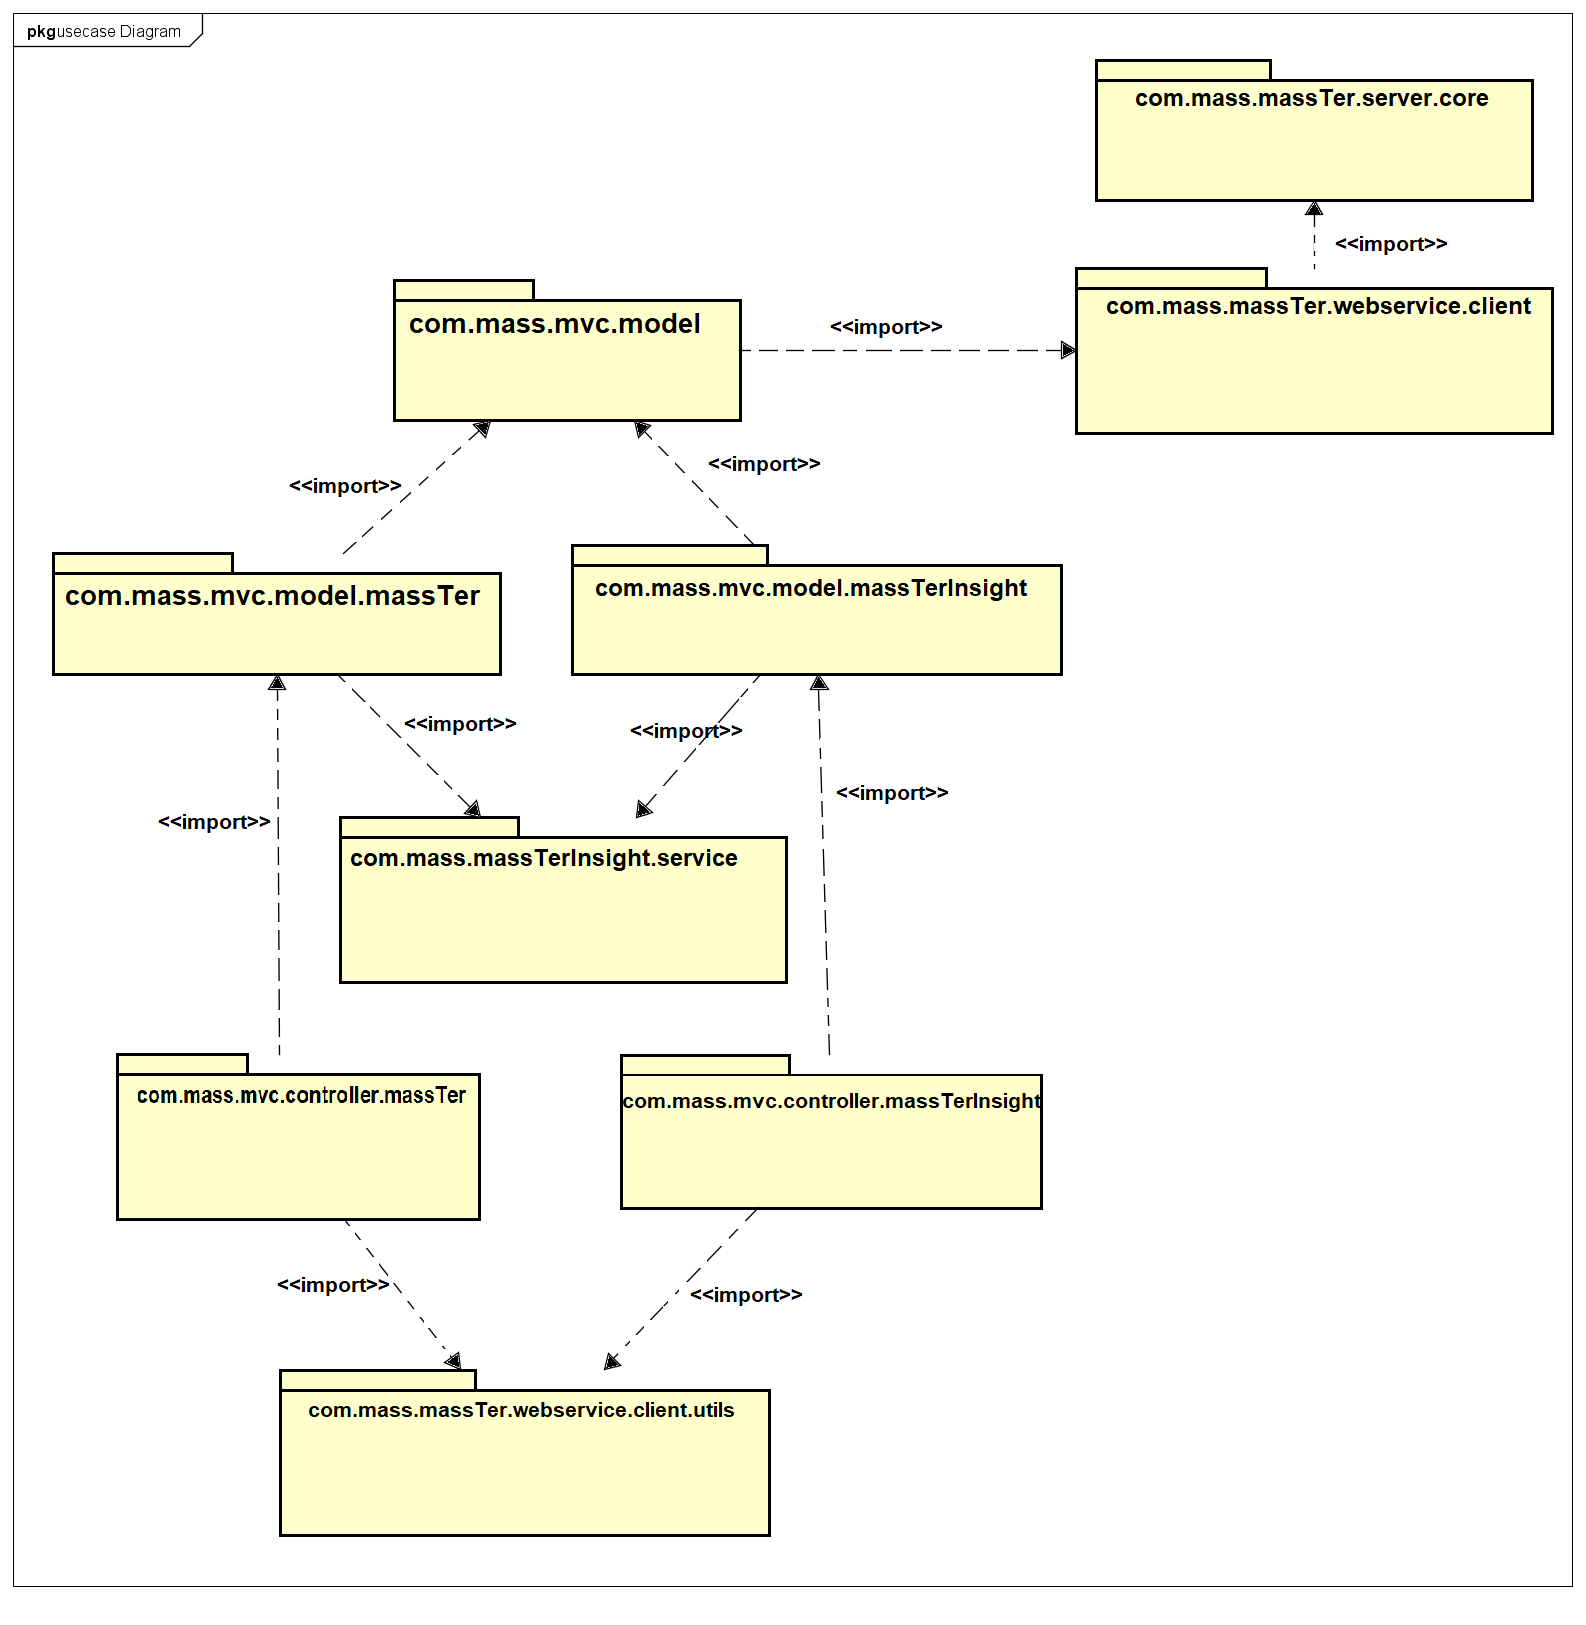
\includegraphics[width=1\textwidth]{packageDiagram.png}
		\caption{package diagram}
	\end{figure}
  
	\pagebreak
	\clearpage
	\newpage
	\subsection{Class Diagram}
			\begin{figure}[h]
		\centering
		\includegraphics[width=17.5cm,height=14cm]{classDiagram.png}
		\caption{Class diagram}
	\end{figure}
	\pagebreak
	\clearpage
	\newpage
	
	\subsection{Sequence Diagram}
		\begin{figure}[h]
		\centering
		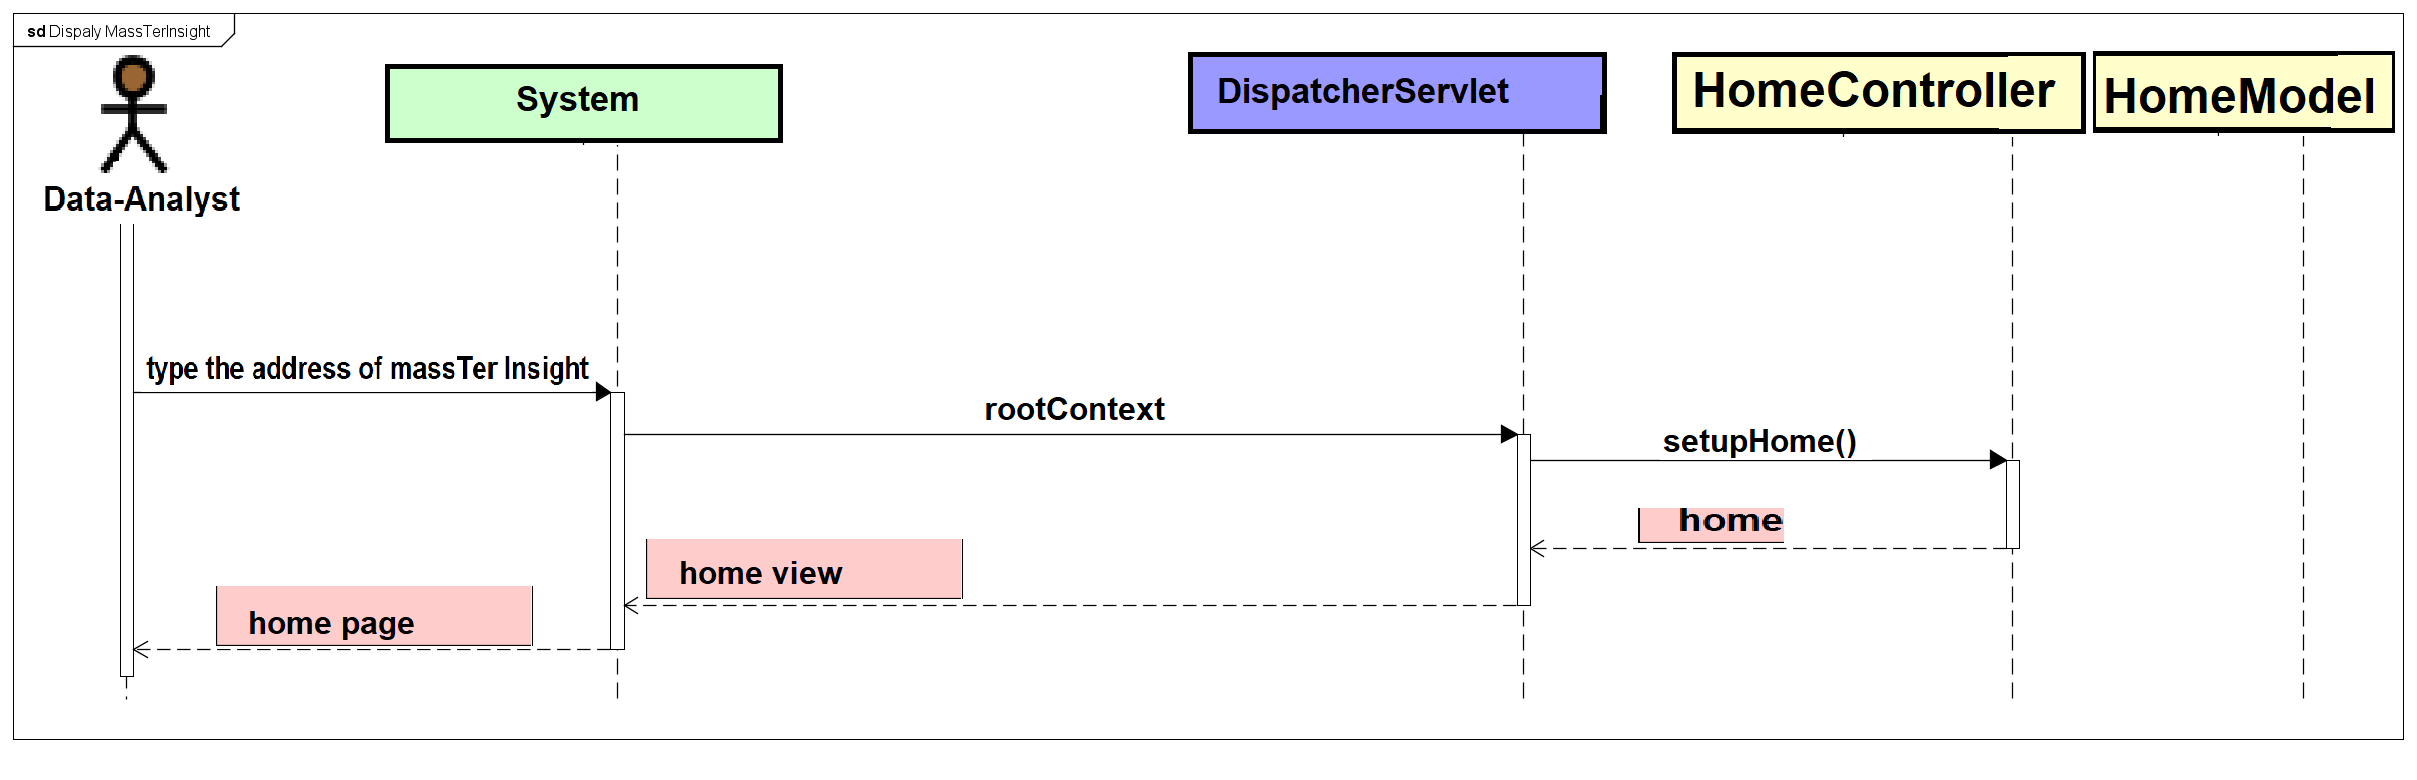
\includegraphics[width=17.5cm,height=8cm]{SequenceDiagramDispalyMassTerInsight.png}
		\caption{Sequence Diagram \textbf{Display MassTerInsight}}
		\end{figure}
	
	\pagebreak
	\clearpage
	\newpage
	\begin{figure}[h]
		\centering
		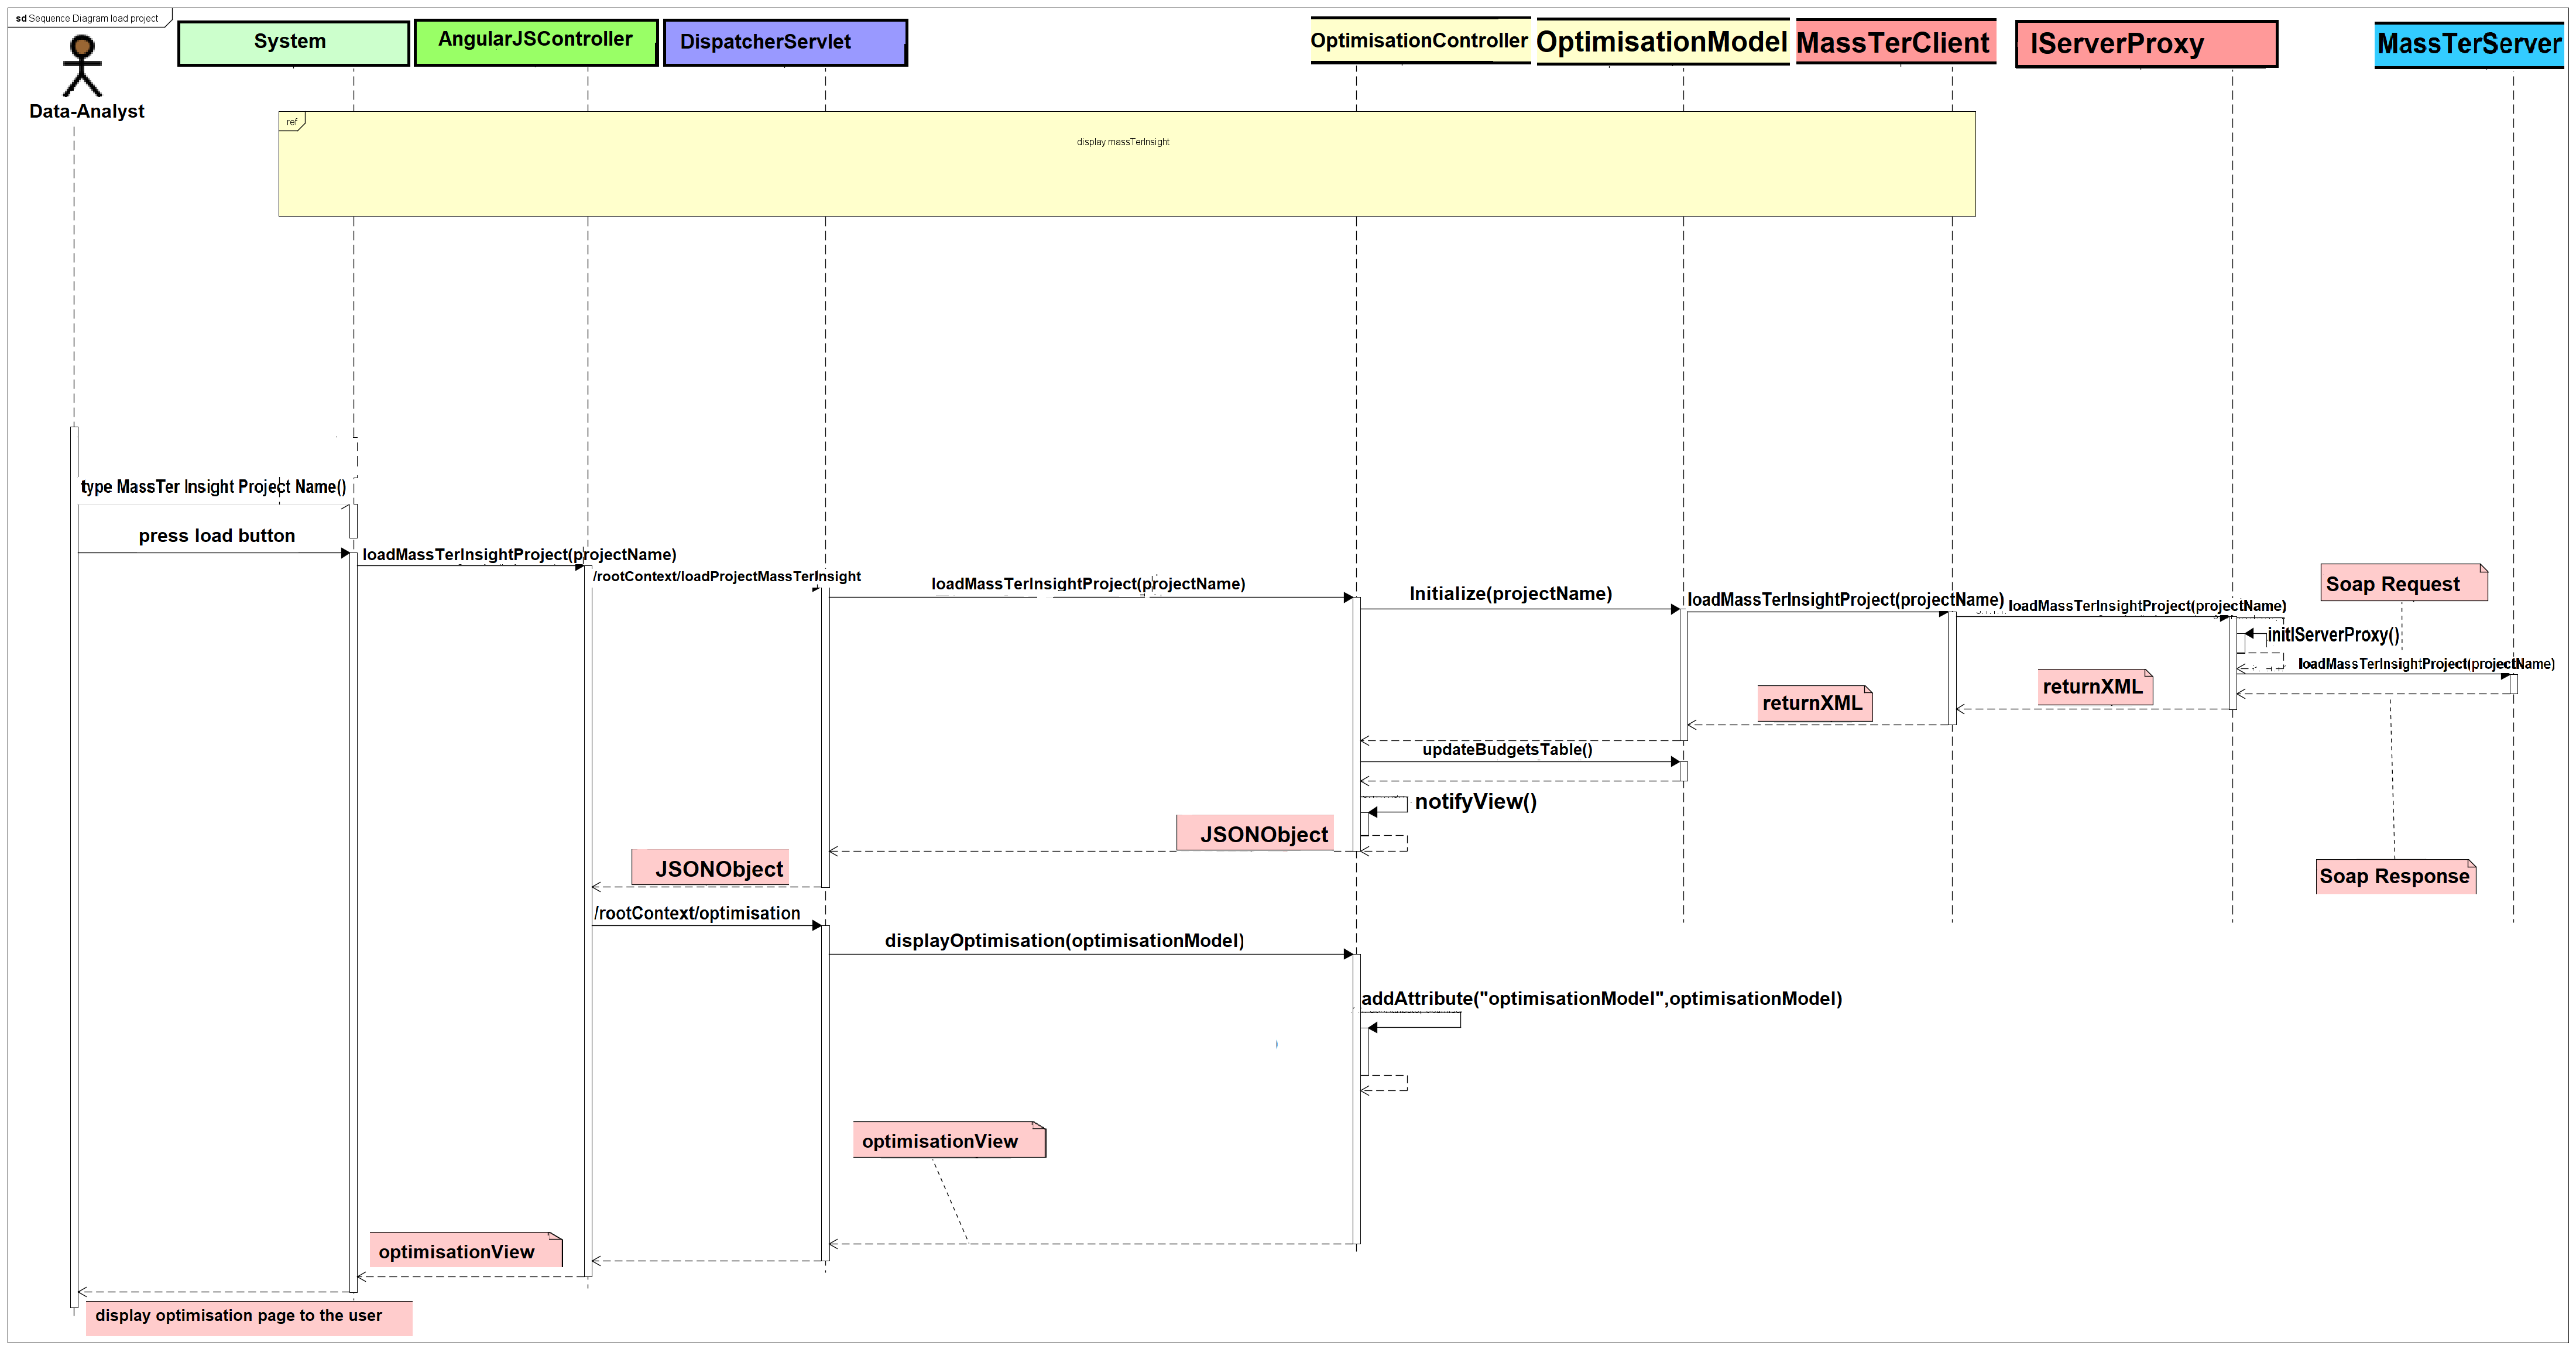
\includegraphics[width=17.5cm,height=17cm]{SequenceDiagramLoadProject.png}
		\caption{Sequence Diagram \textbf{Load MassTerInsight Project Use Case}}
	\end{figure}
    
    \pagebreak
	\clearpage
	\newpage

	\begin{figure}[h]
		\centering
		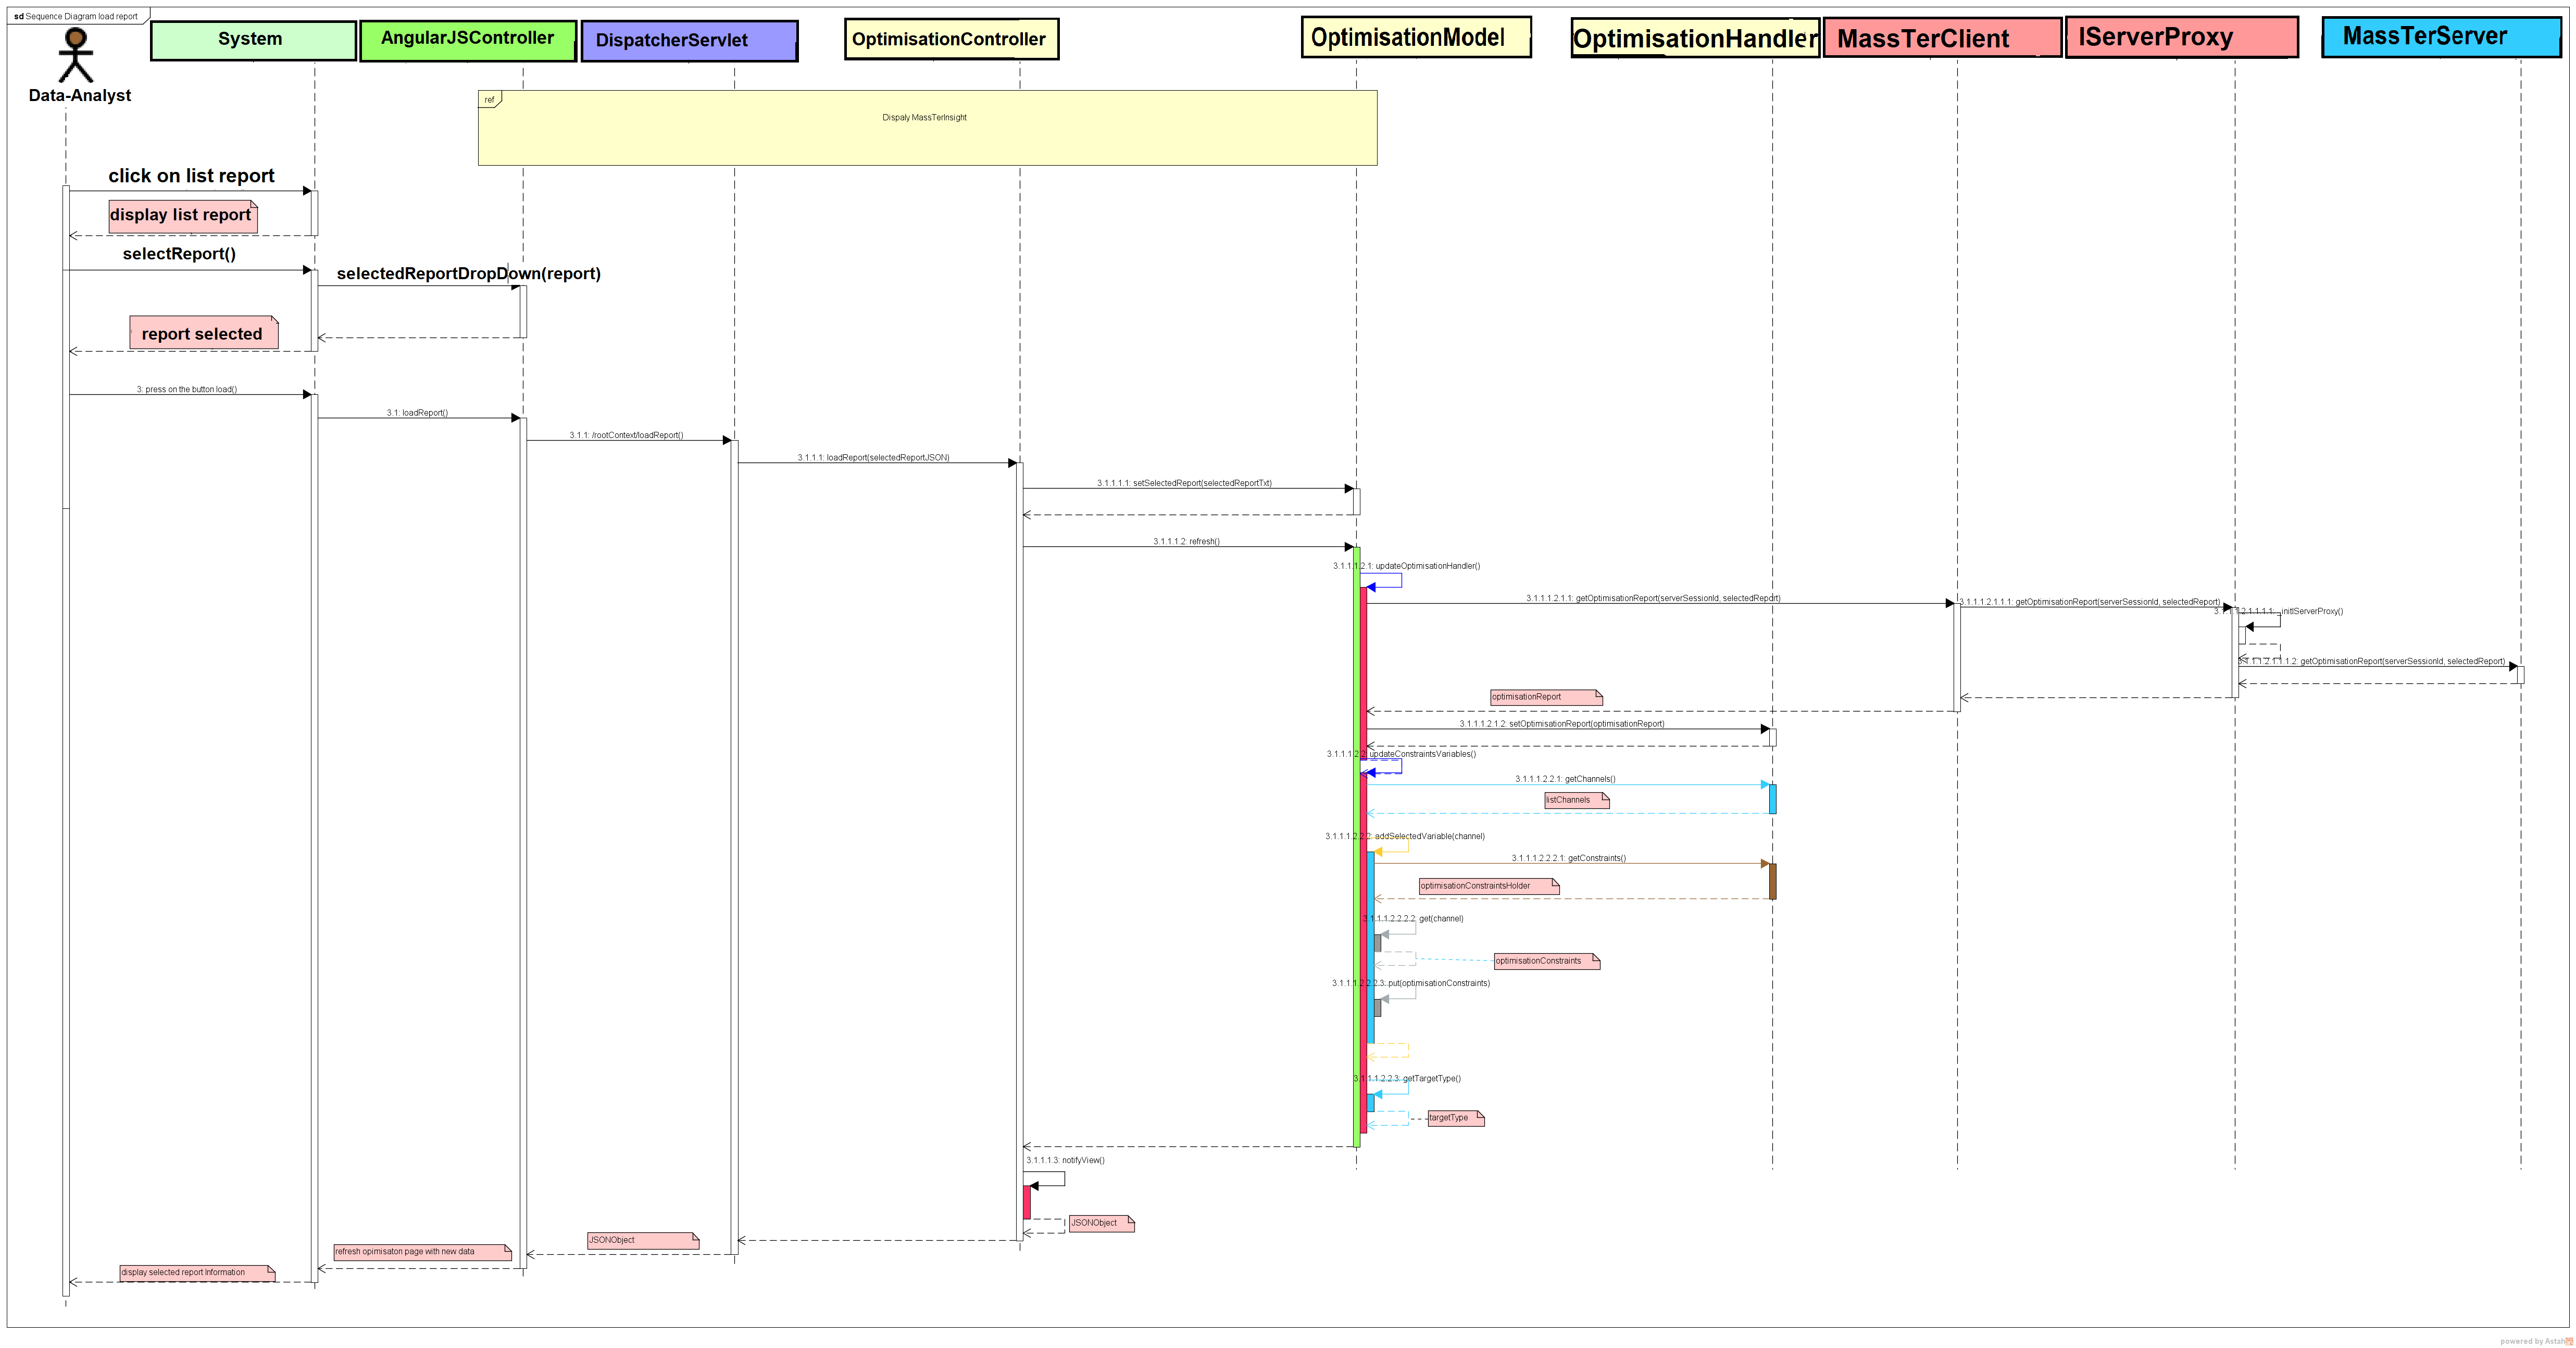
\includegraphics[width=17.5cm,height=17cm]{SequenceDiagramLoadReport.png}
		\caption{Sequence Diagram \textbf{Load Report Use Case}}
	\end{figure}


	\pagebreak
	\clearpage
	\newpage

	\begin{figure}[h]
		\centering
		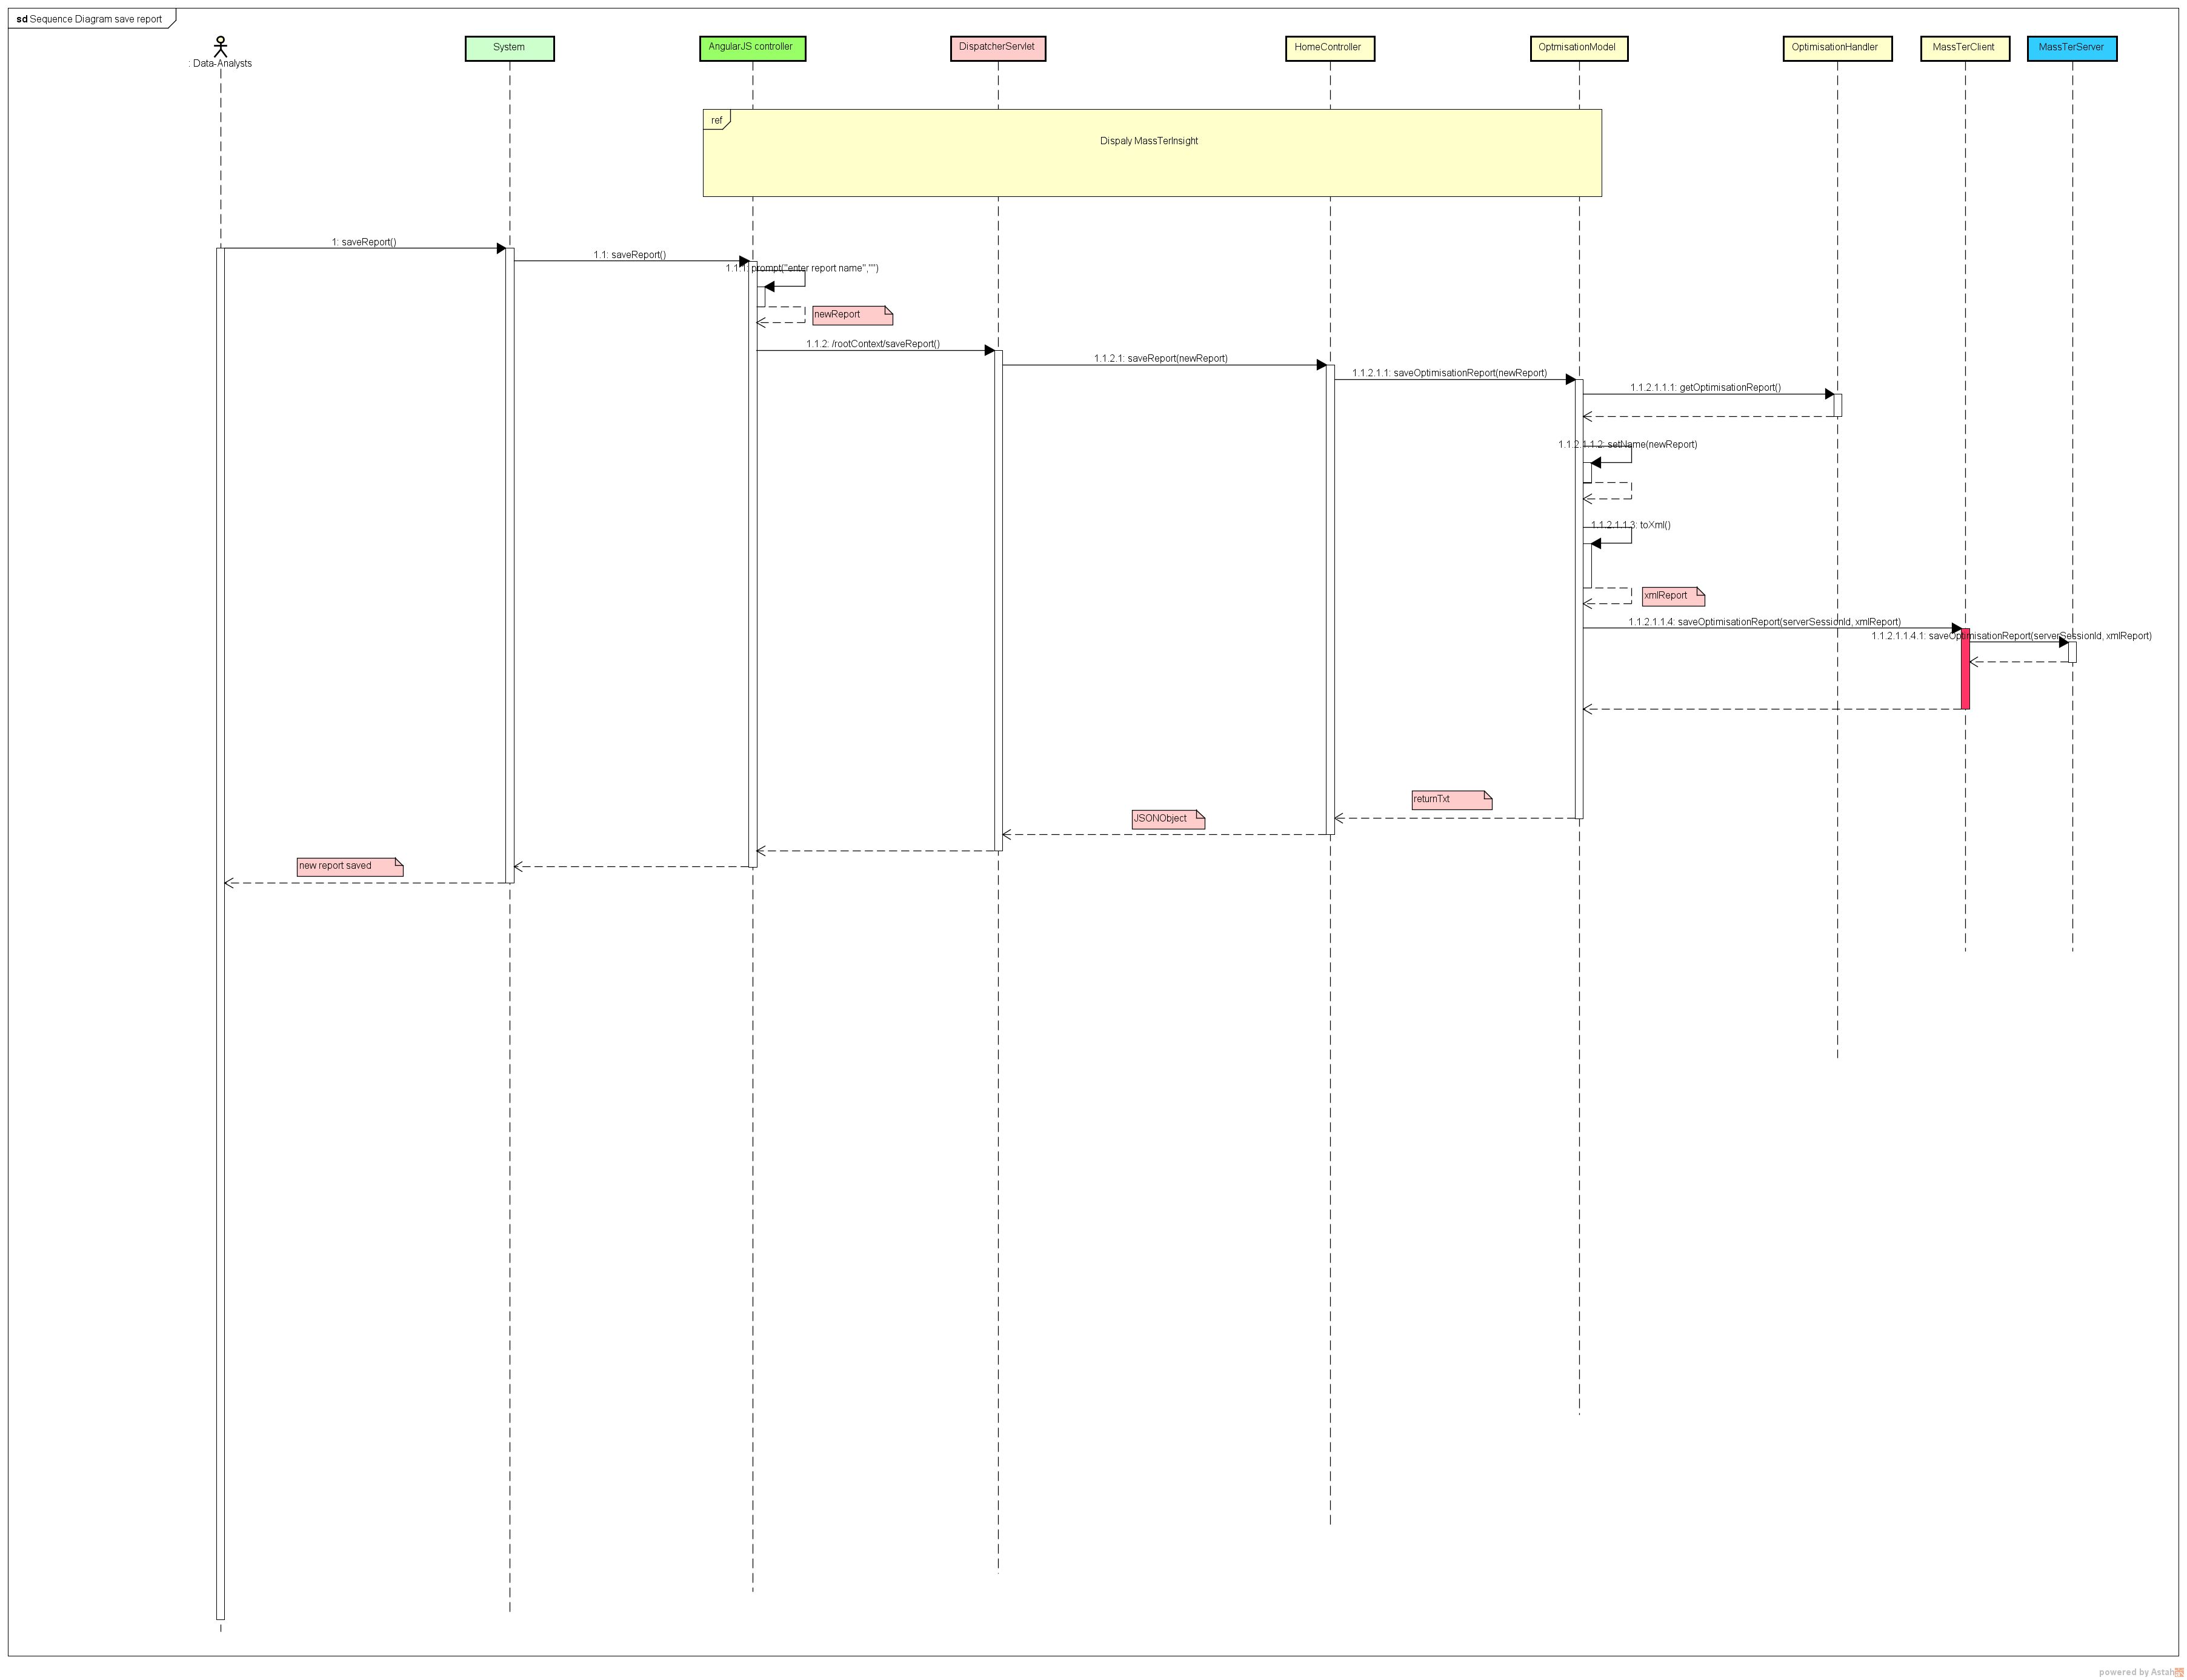
\includegraphics[width=17.5cm,height=17cm]{SequenceDiagramSaveReport.png}
		\caption{Sequence Diagram \textbf{Save Report Use Case}}
	\end{figure}
	
	\pagebreak
	\clearpage
	\newpage 

   \begin{figure}[h]
   	\centering
   	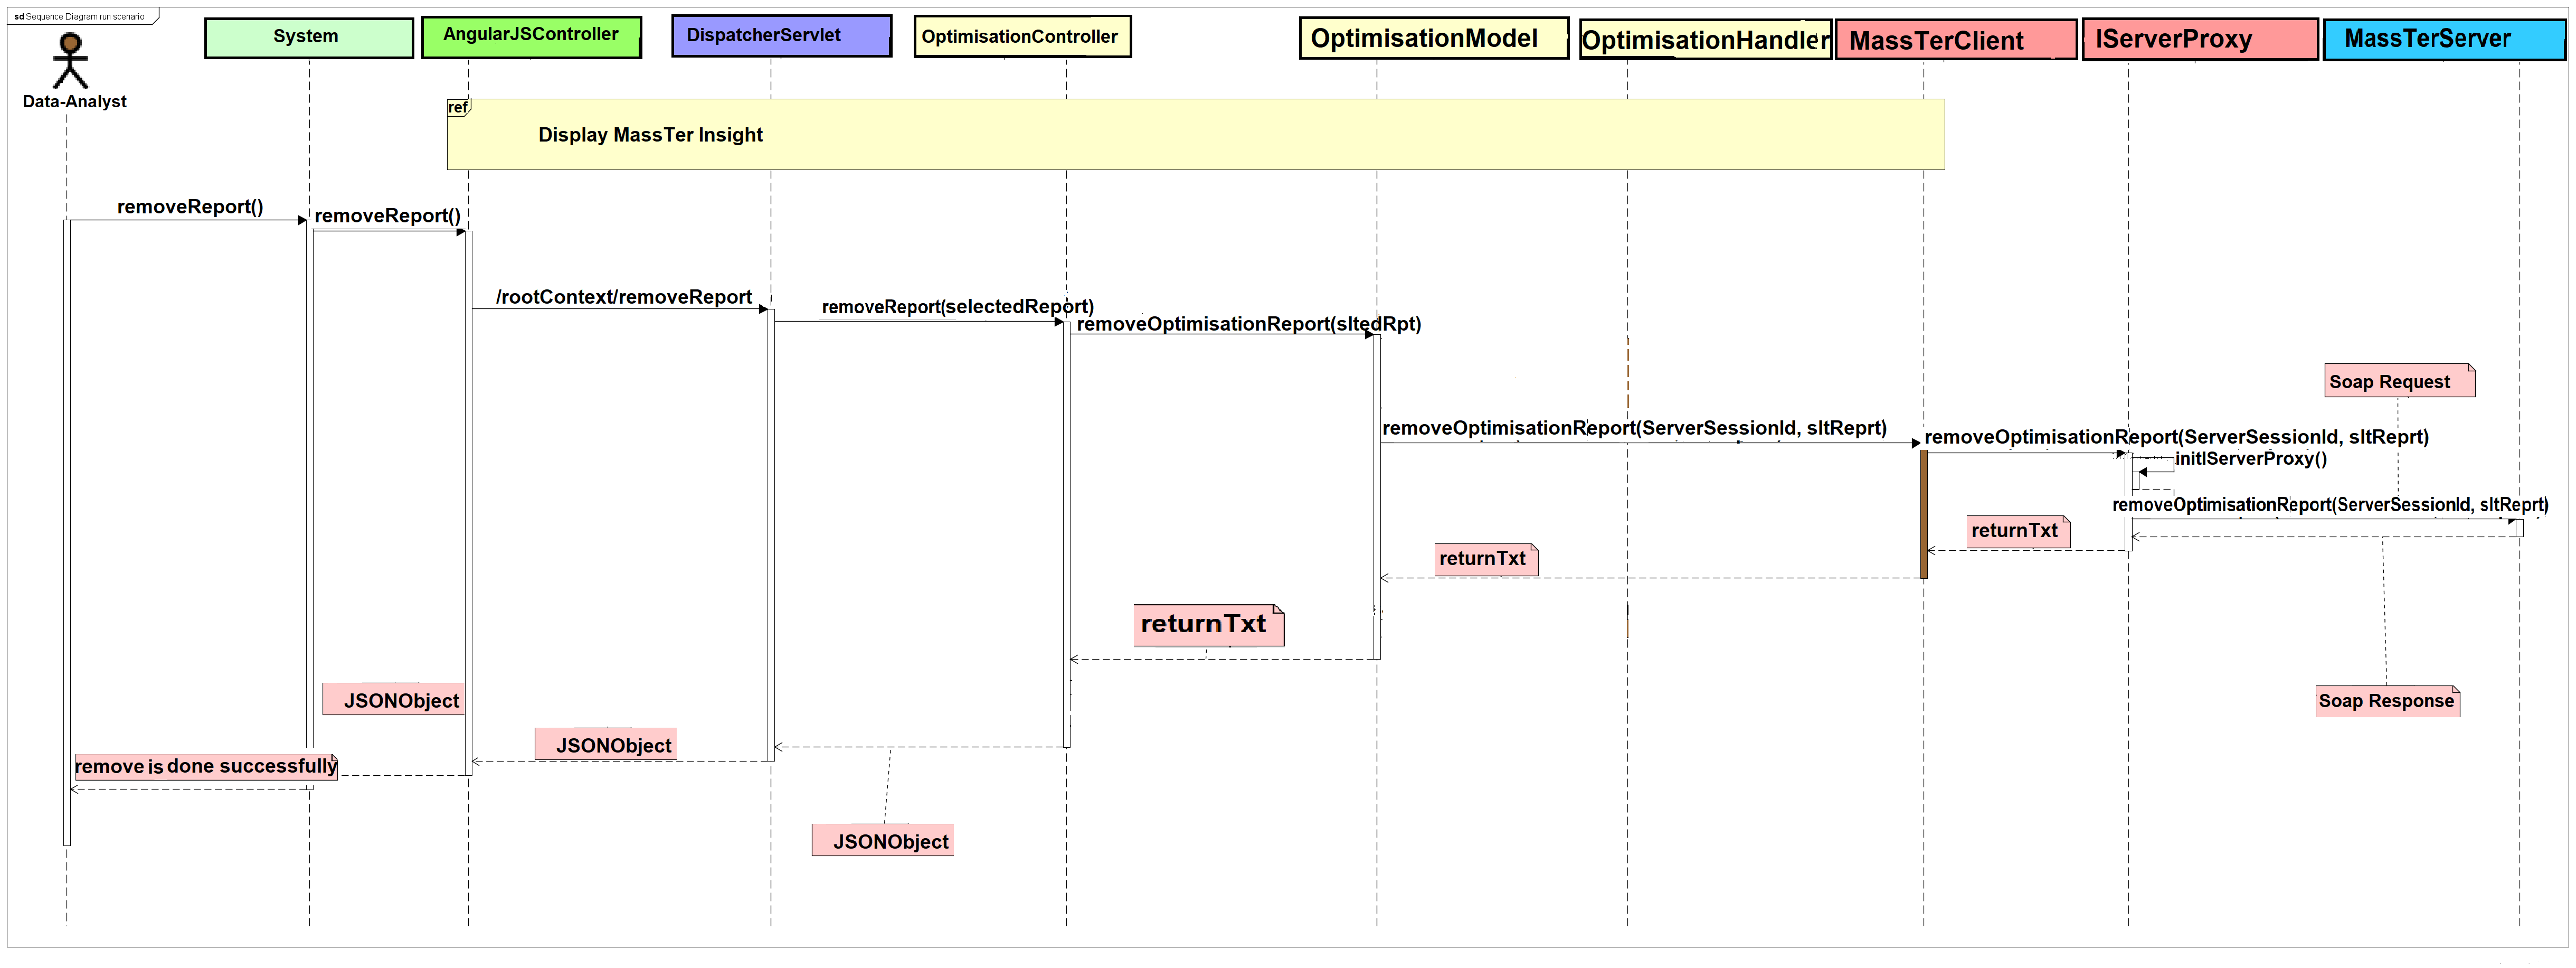
\includegraphics[width=17.5cm,height=17cm]{SequenceDiagramRemoveReport.png}
   	\caption{Sequence Diagram \textbf{Remove Report Use Case}}
   \end{figure}
	
	\pagebreak
	\clearpage
	\newpage
	
	\begin{figure}[h]
		\centering
		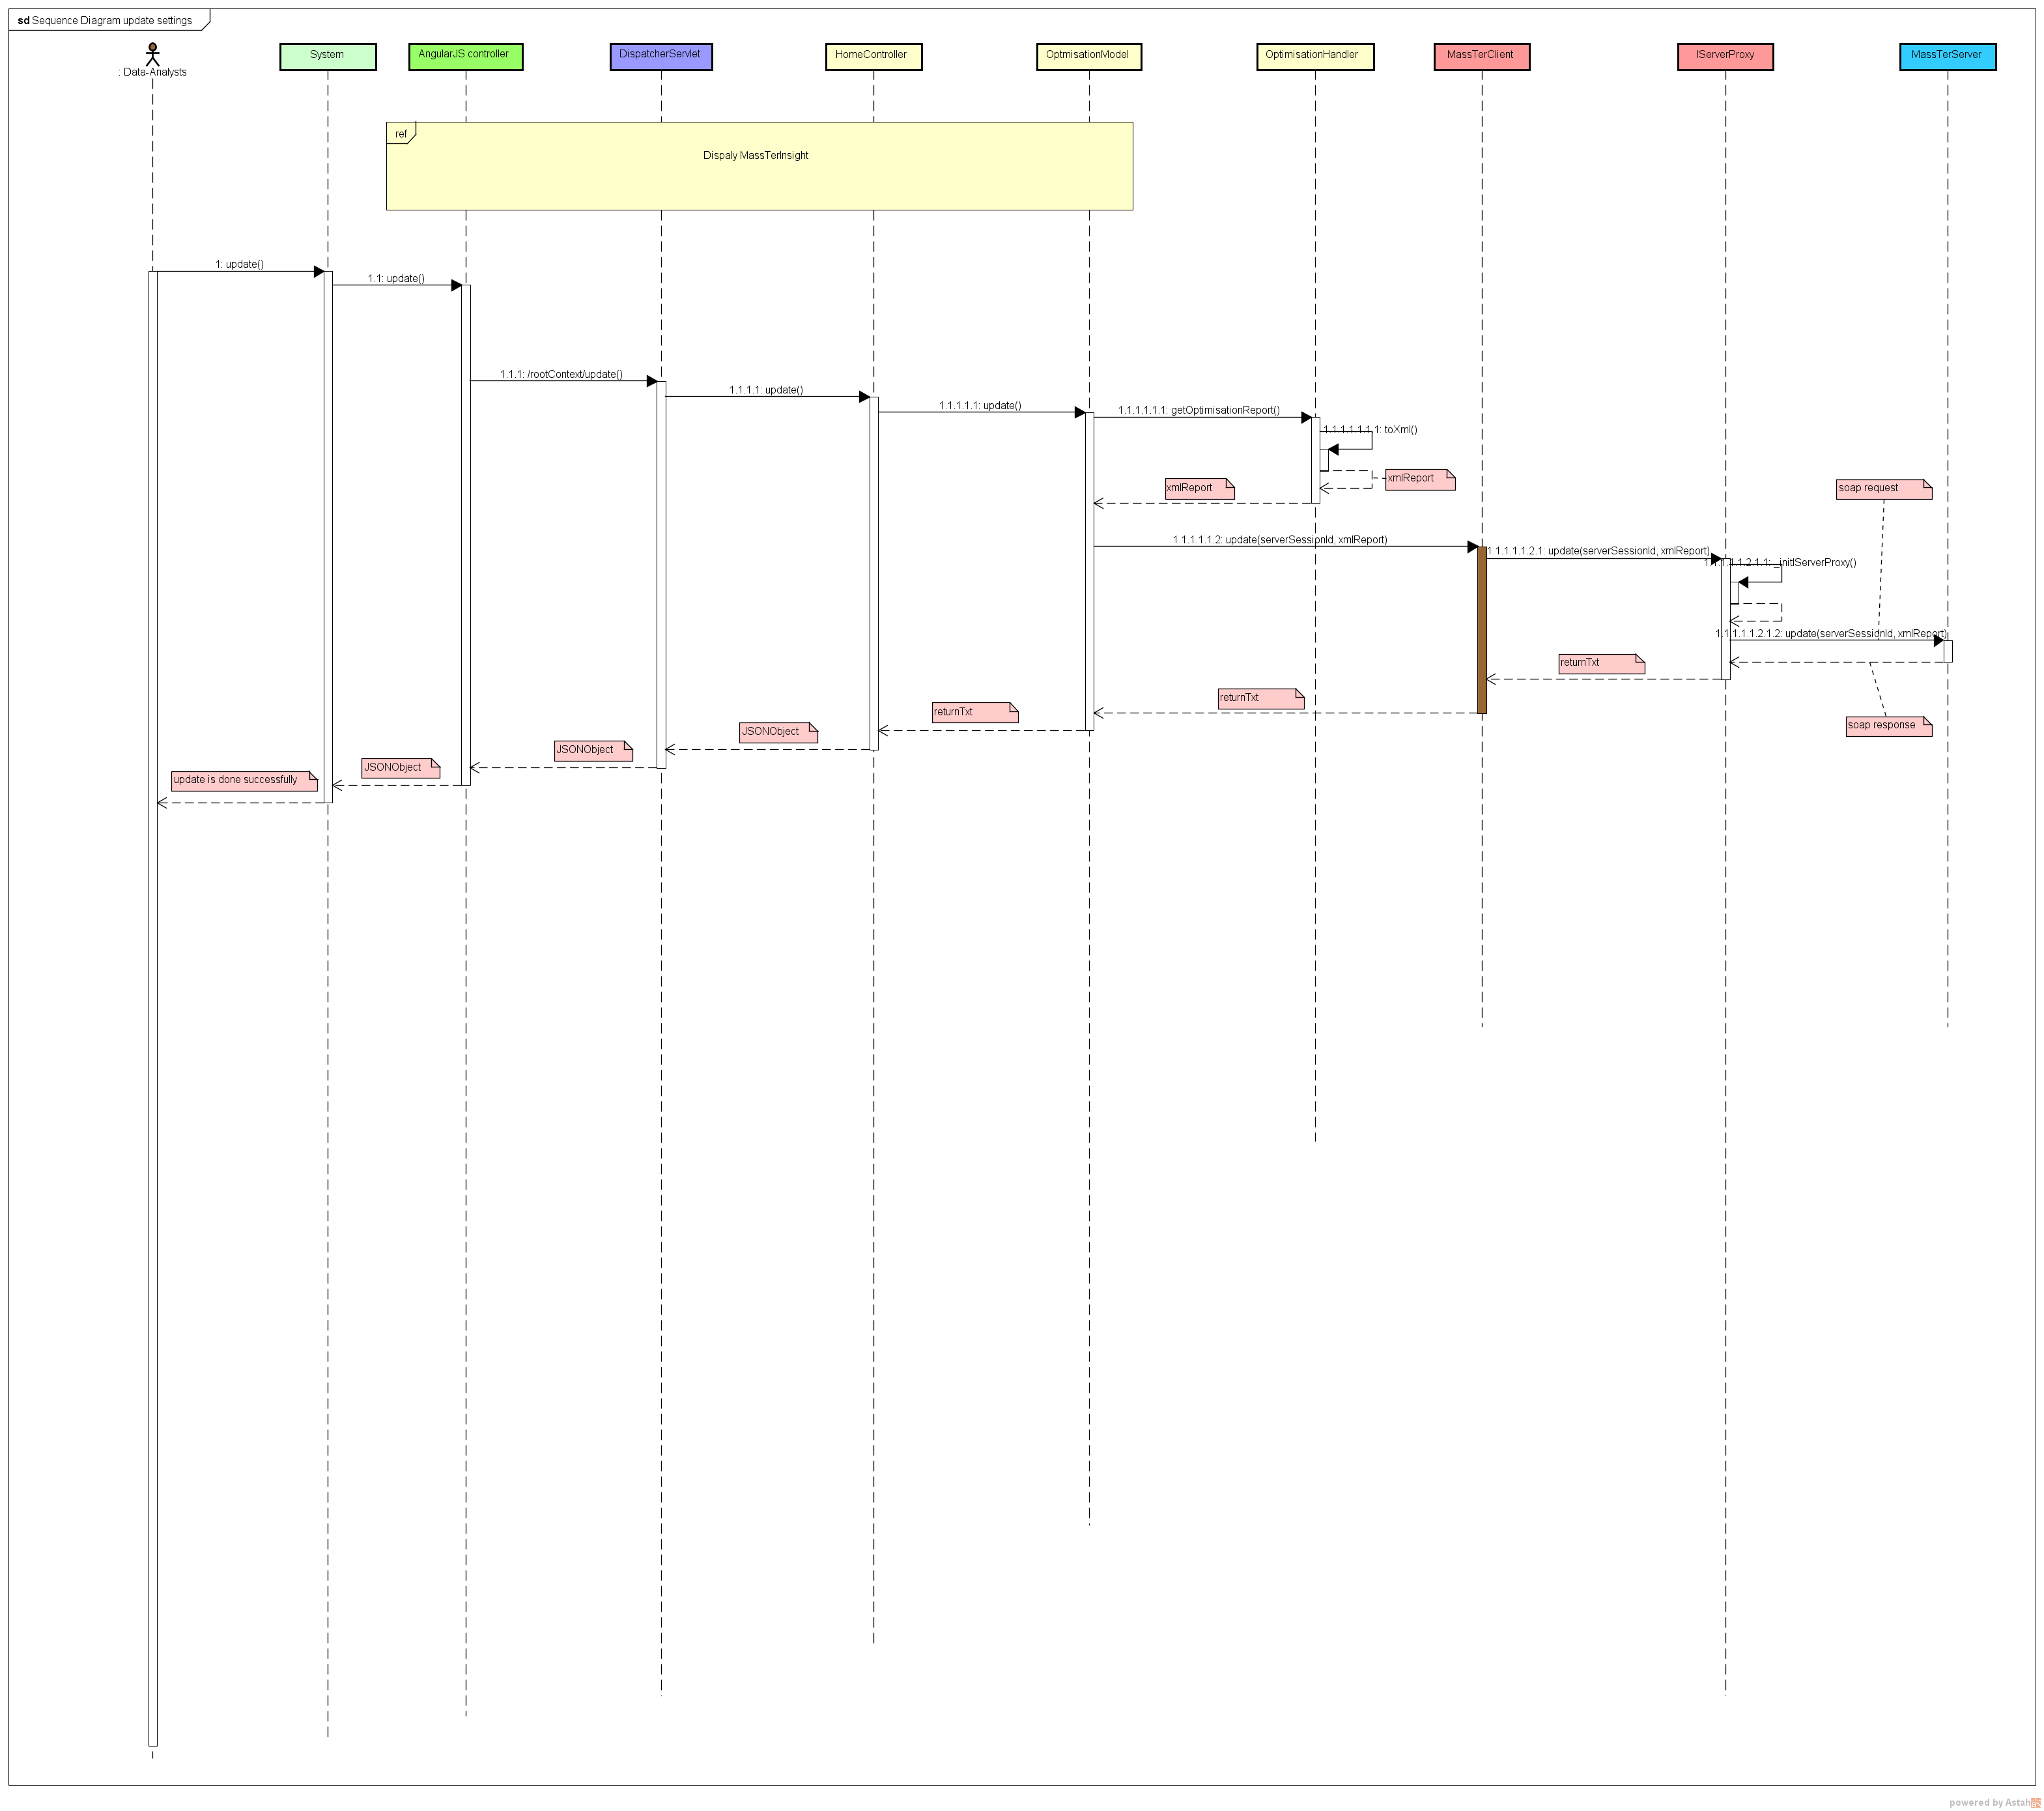
\includegraphics[width=17.5cm,height=17cm]{SequenceDiagramUpdateSettings.png}
		\caption{Sequence Diagram \textbf{update settings Use Case}}
	\end{figure}

	
	\pagebreak
	\clearpage
	\newpage
	
	\begin{figure}[h]
	\centering
	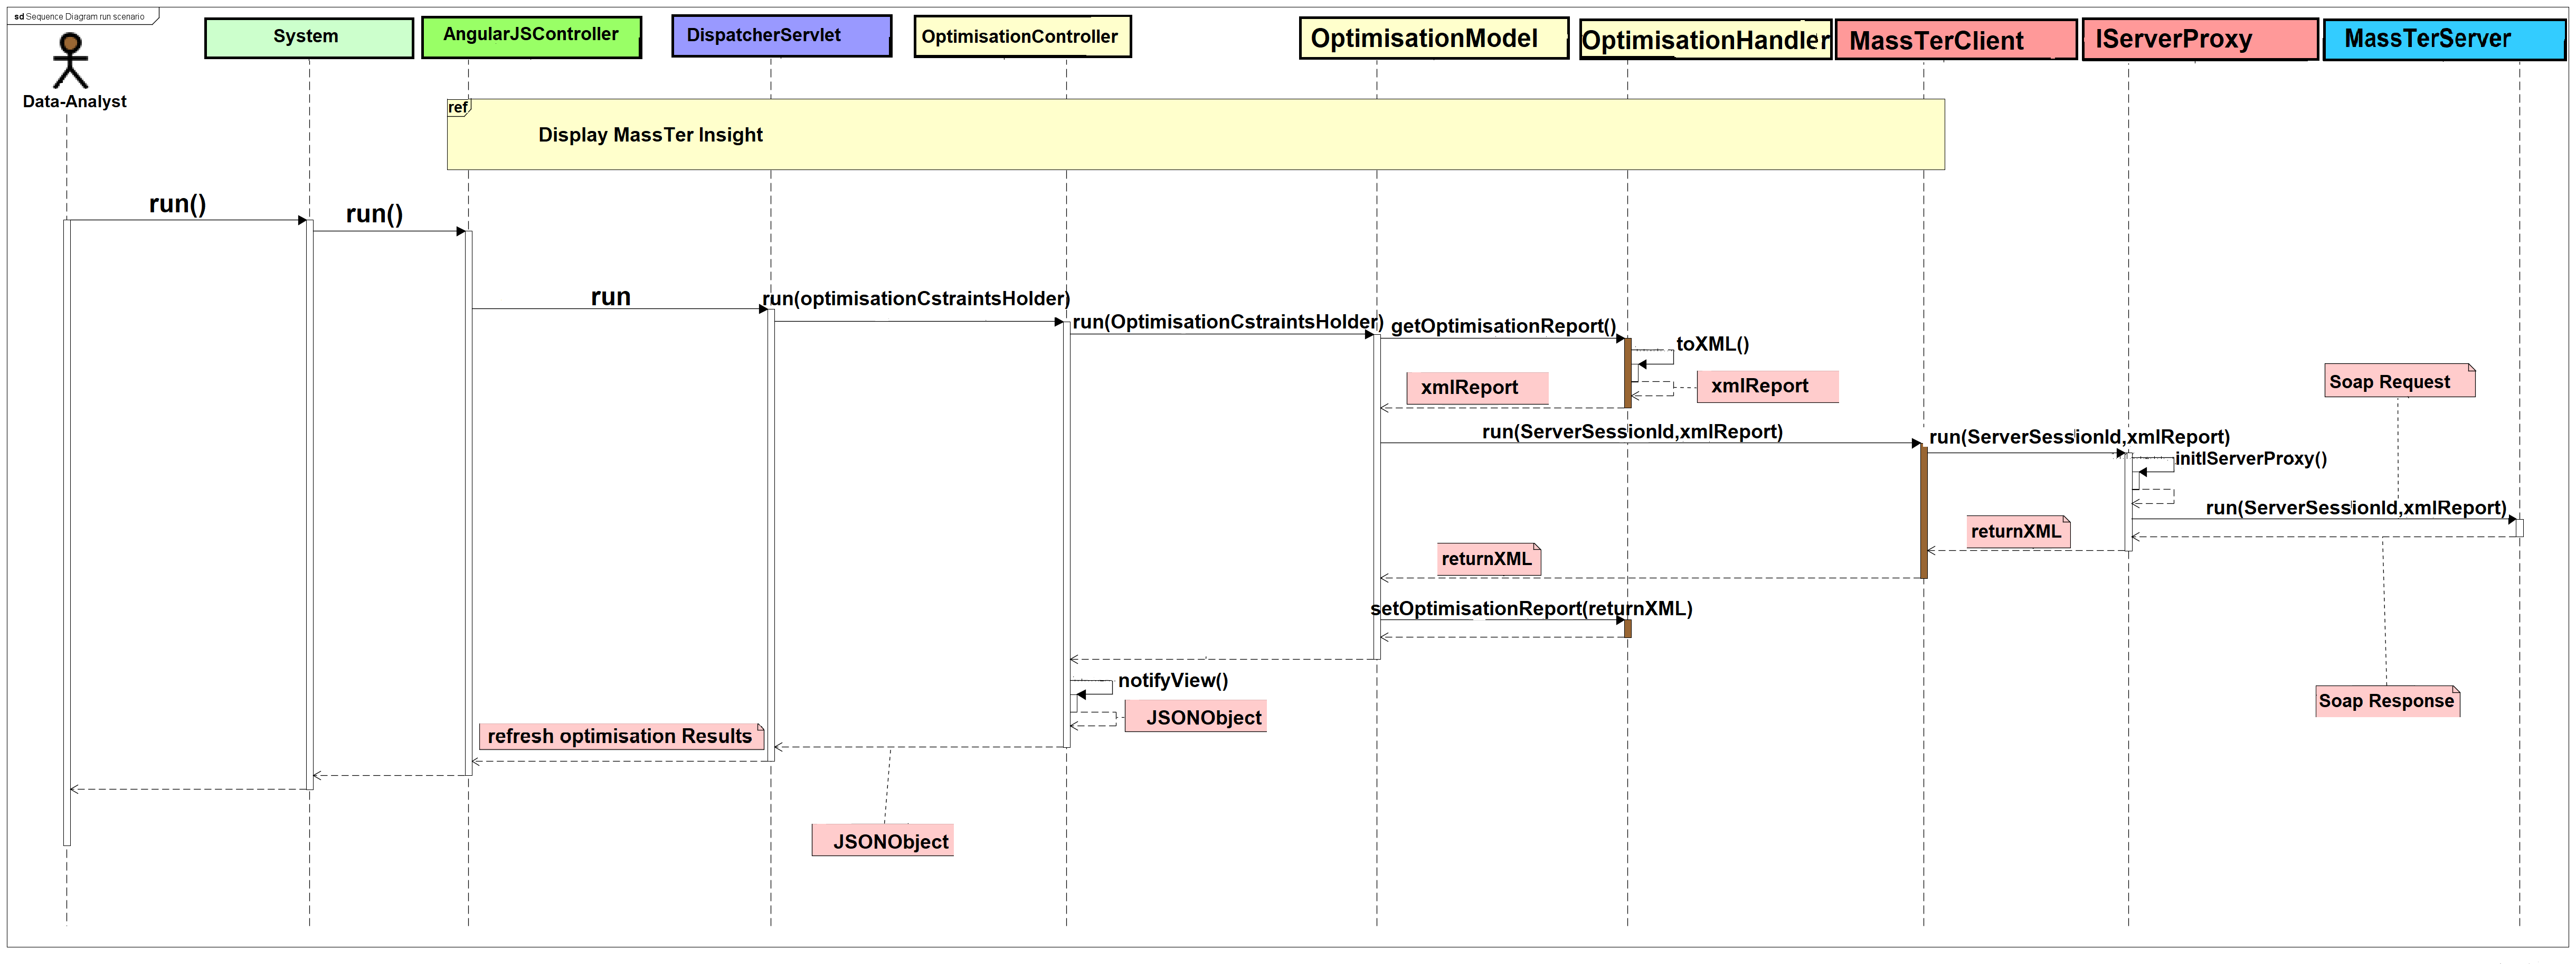
\includegraphics[width=17.5cm,height=17cm]{SequenceDiagramRunScenario.png}
	\caption{Sequence Diagram \textbf{Run Scenario Use Case}}
    \end{figure}
	
	\pagebreak
	\clearpage
    \newpage 
	
	\begin{figure}[h]
		\centering
		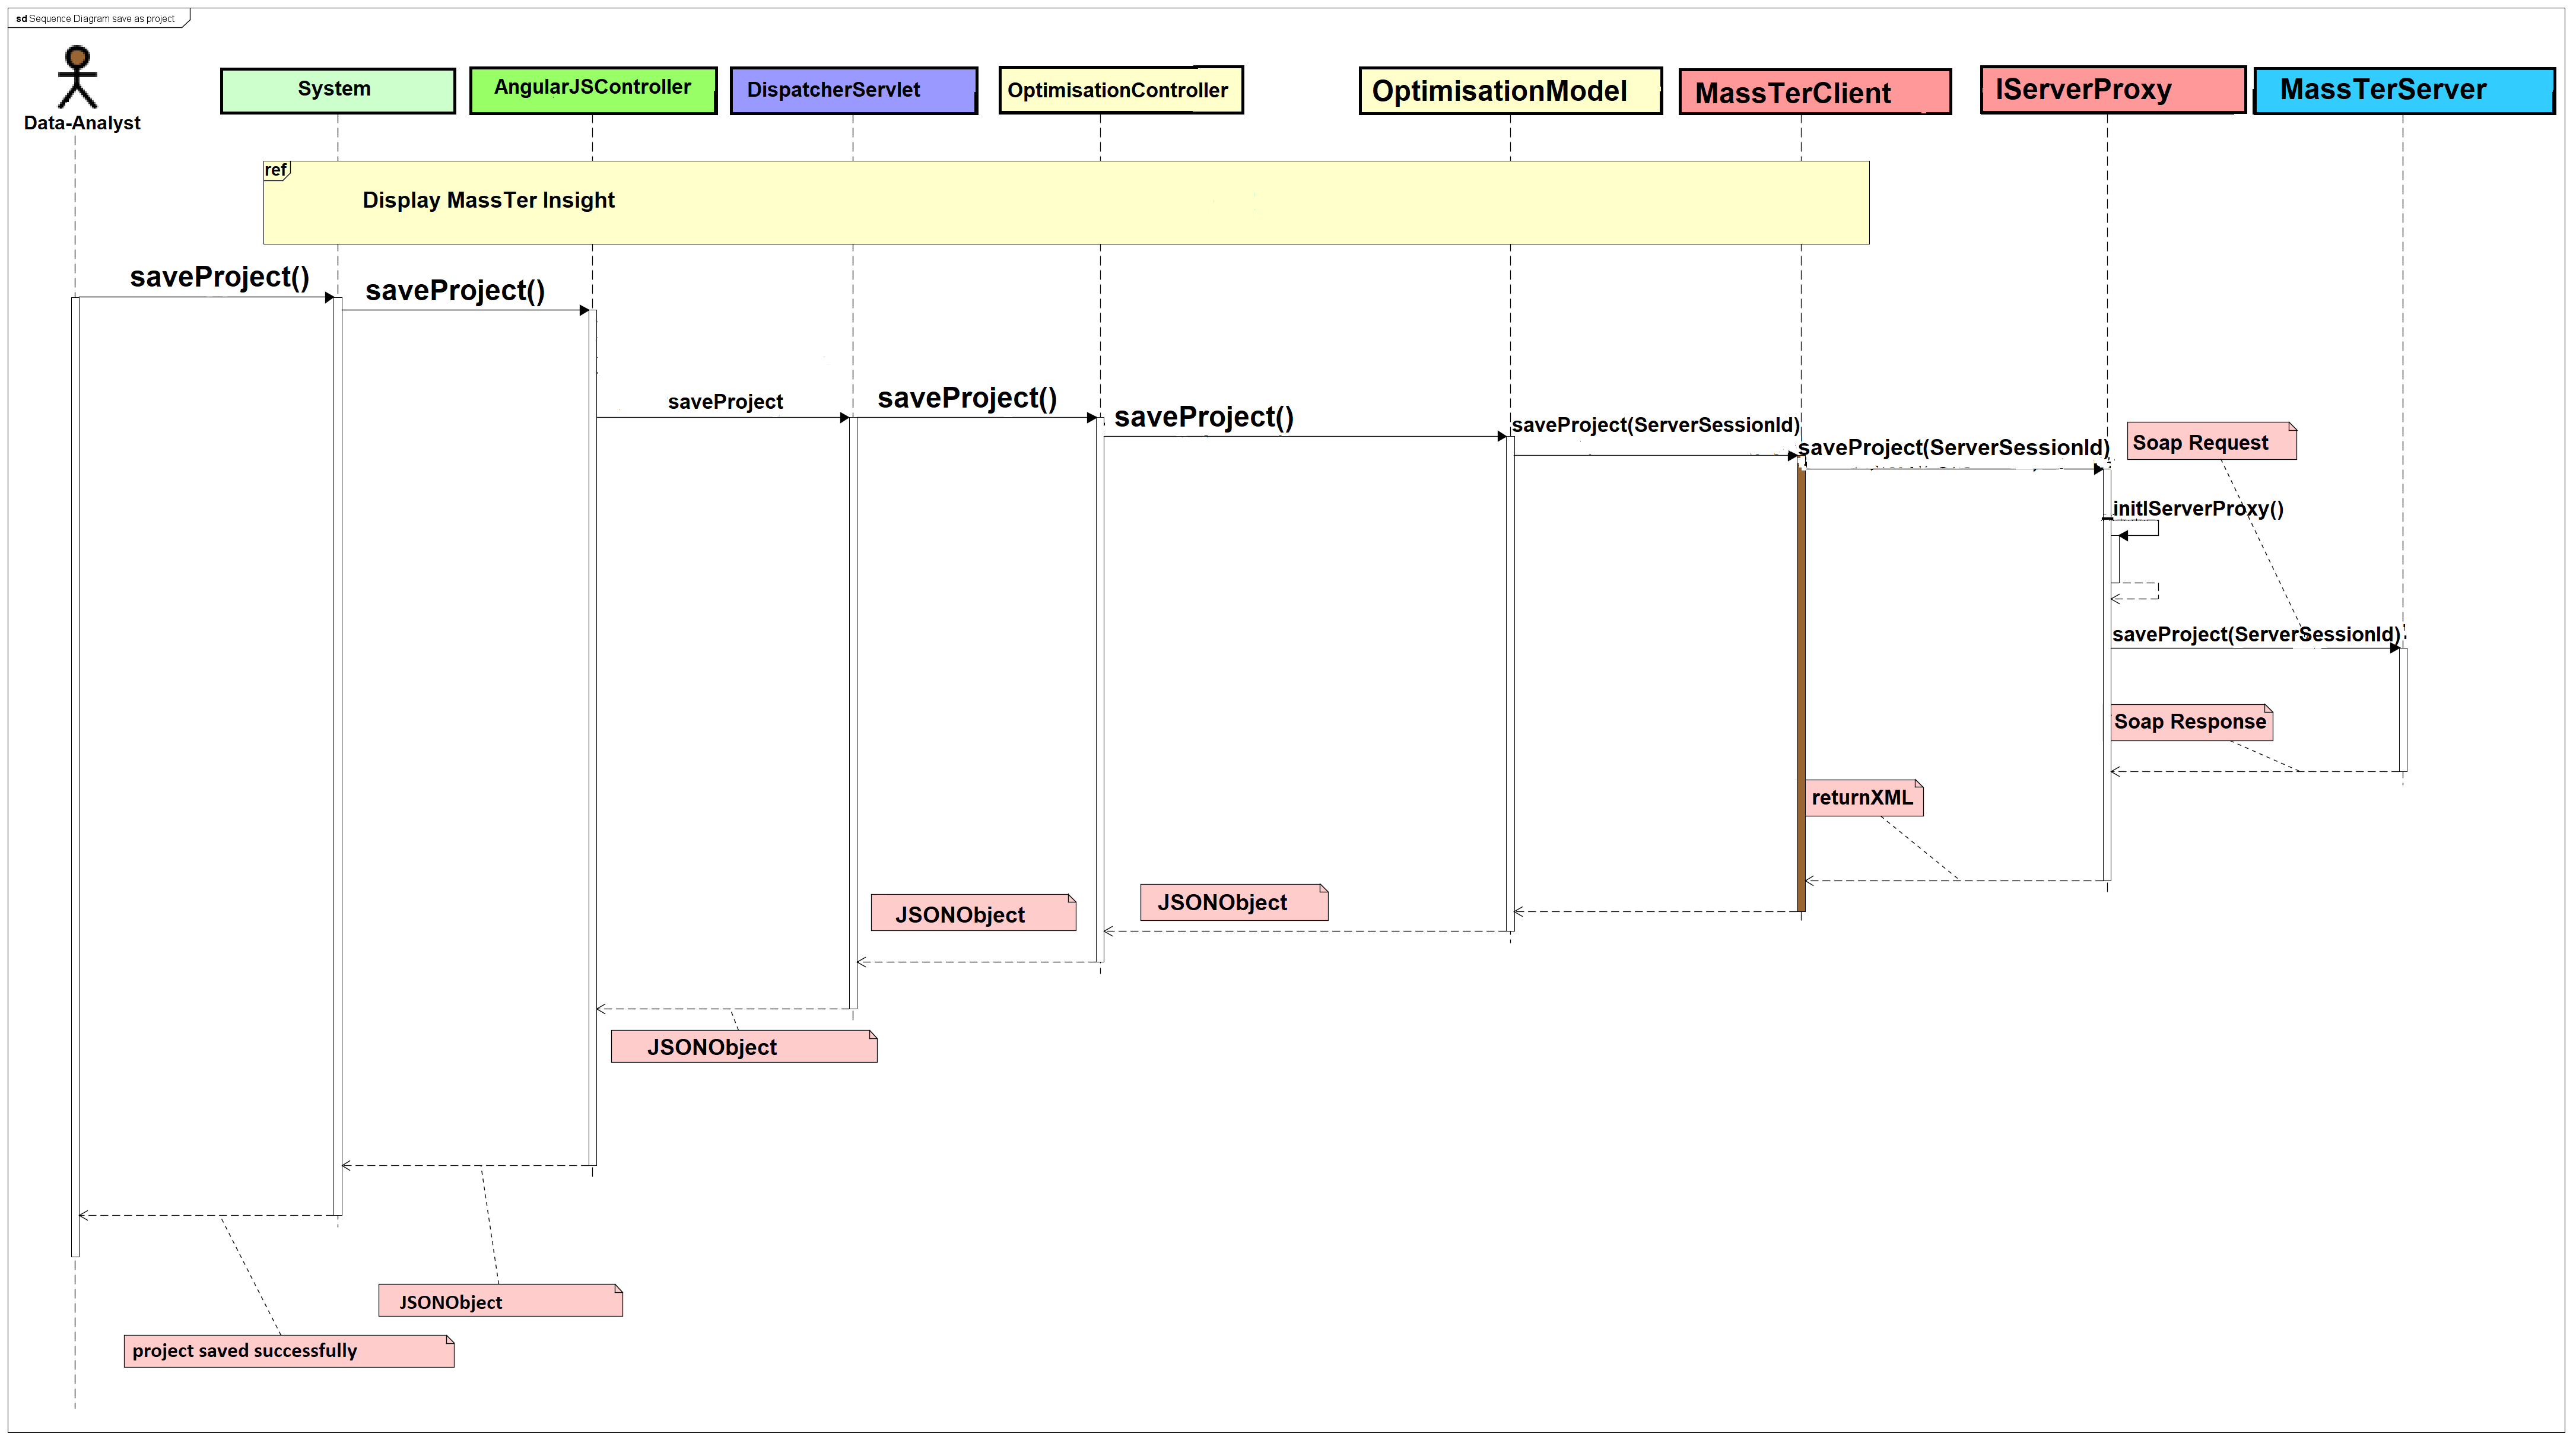
\includegraphics[width=17.5cm,height=17cm]{SequenceDiagramSaveProject.png}
		\caption{Sequence Diagram \textbf{Save Project Use Case}}
	\end{figure}

	
    \pagebreak
	\clearpage
	\newpage
	\begin{figure}[h]
	\centering
	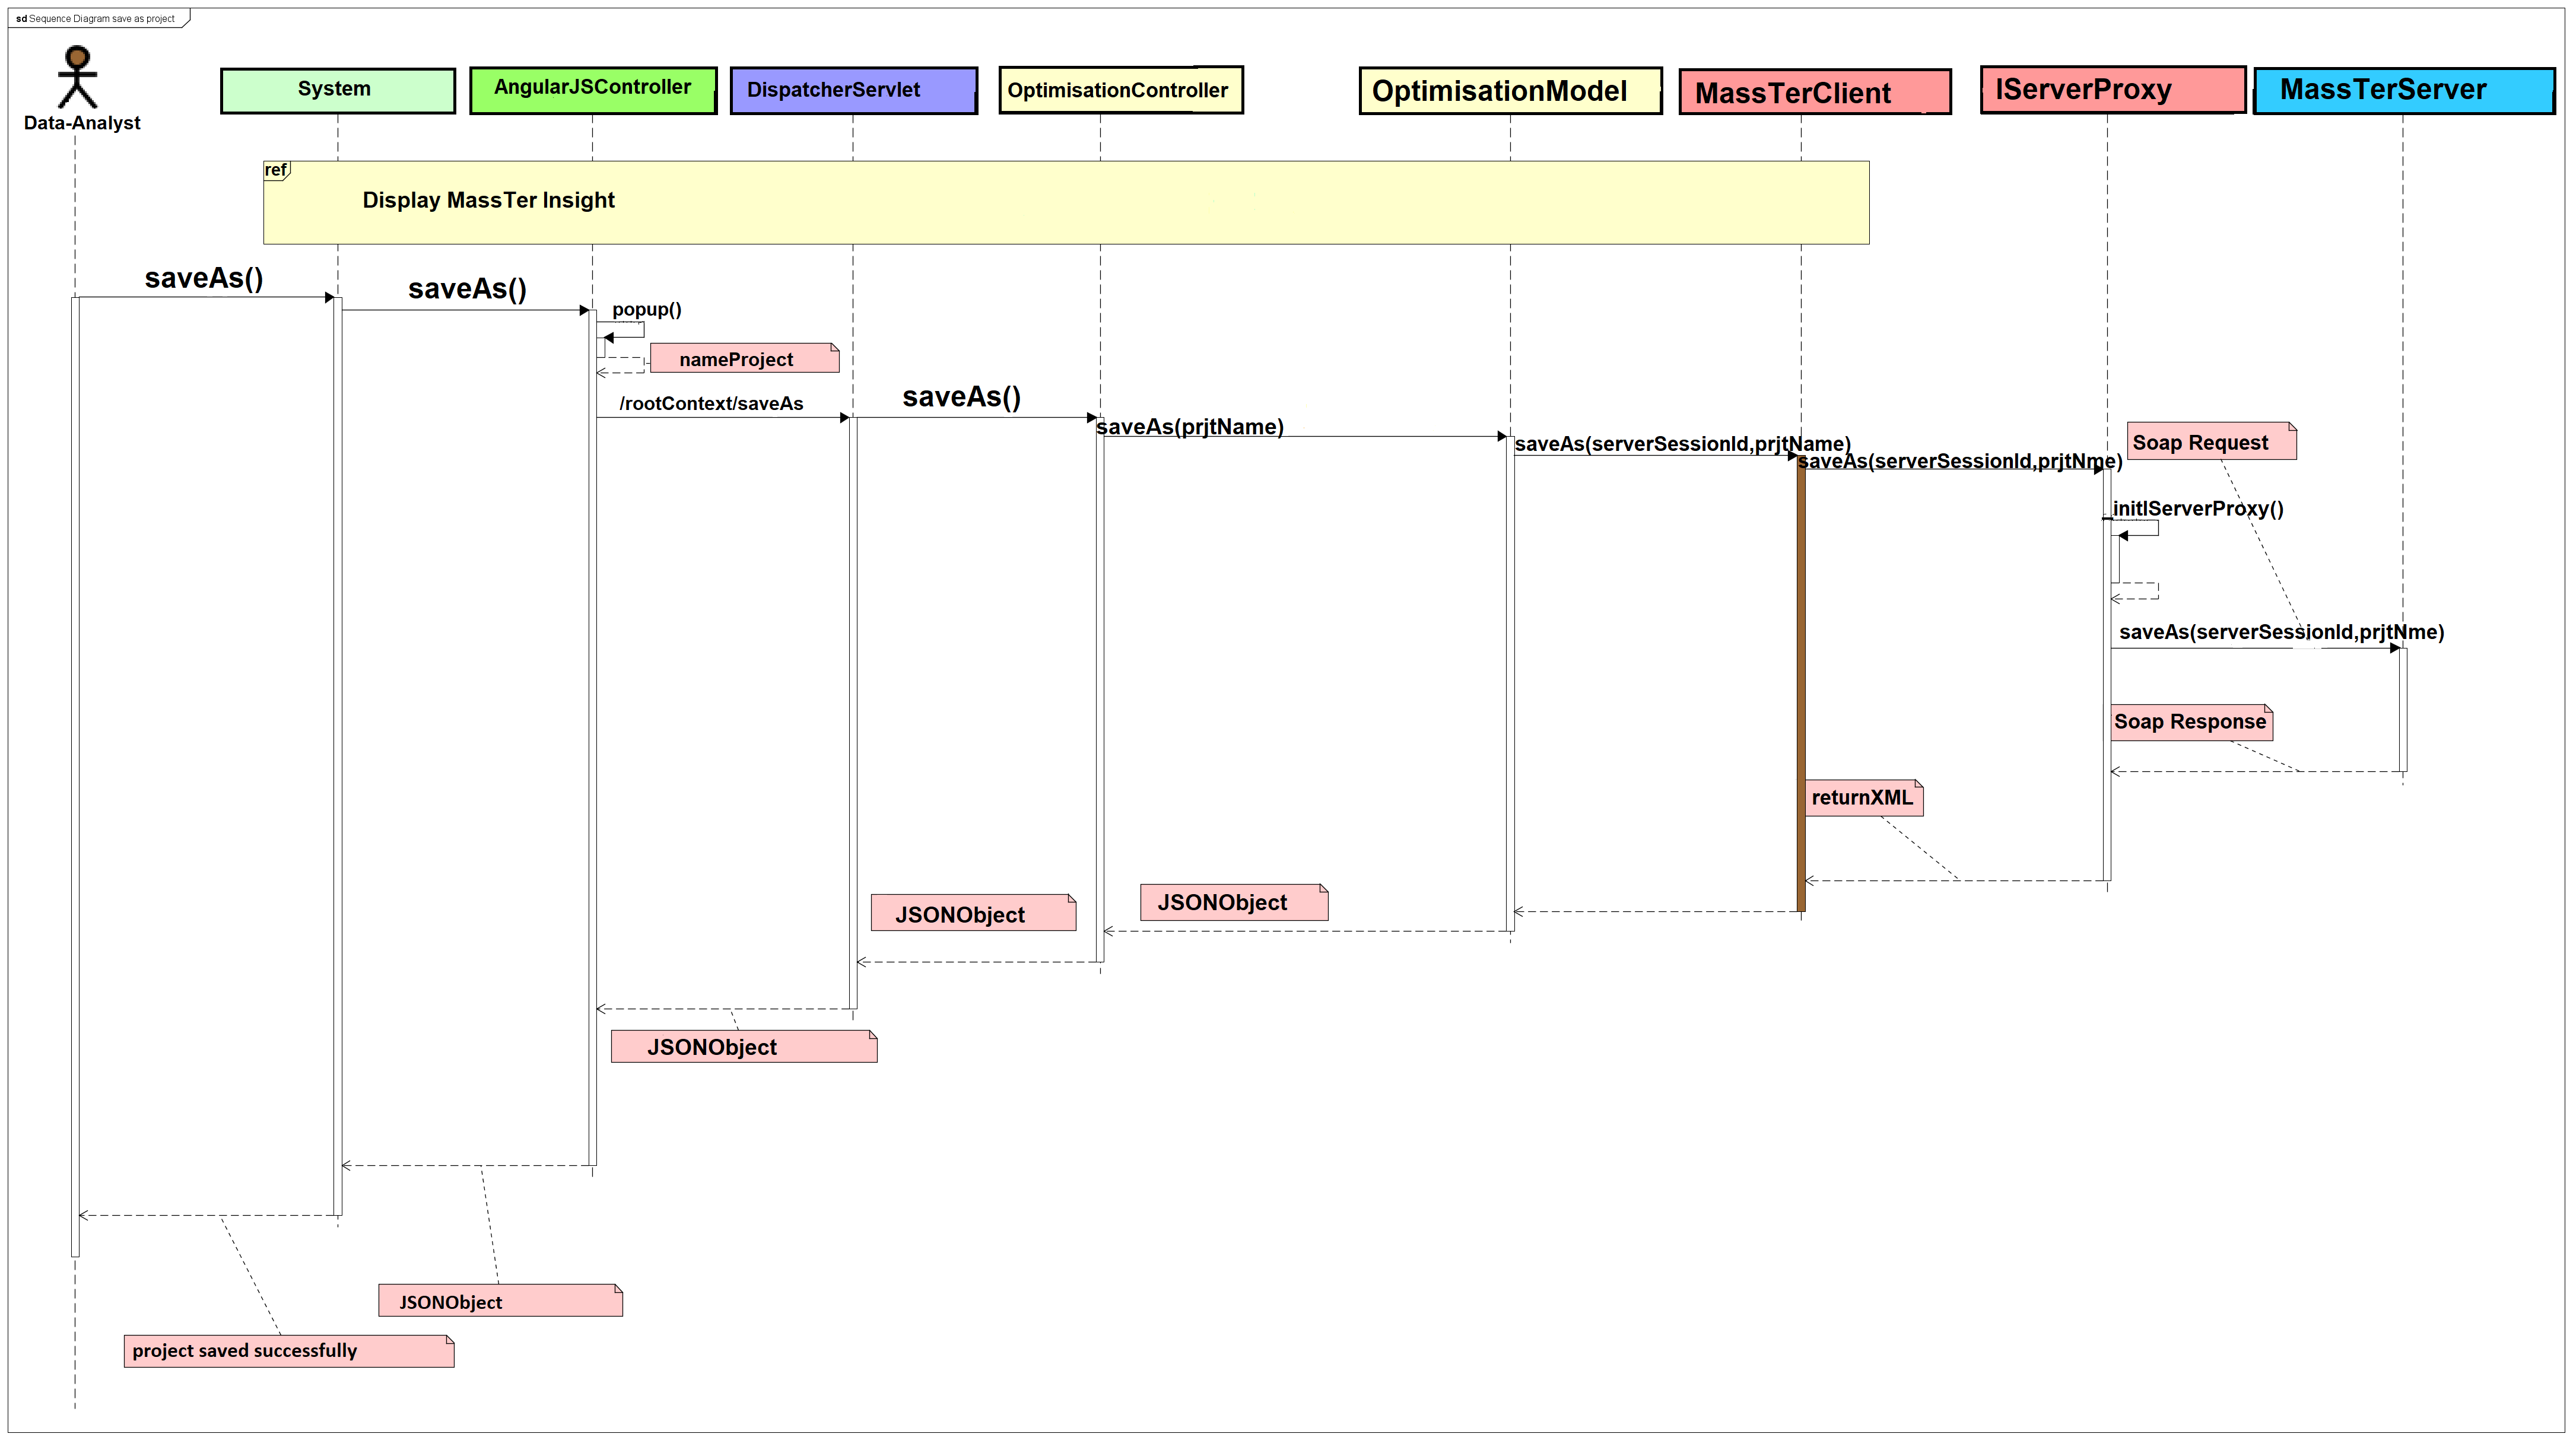
\includegraphics[width=17.5cm,height=17cm]{SequenceDiagramSaveAsProject.png}
	\caption{Sequence Diagram \textbf{Save As Project Use Case}}
    \end{figure}
    
 \pagebreak
\clearpage
\newpage
 \pagebreak
\clearpage
\newpage
	\section{Conclusion}
	Throughout this chapter, we have dissected the application to achieve gradually.
	We started by presenting the general architecture of the application, then we explained the global conception, unveiled through the packages diagrams, to go then to the detailed conception using class diagram and the sequences diagrams.  

	
		% include chapter 4 %
	\clearpage
	\newpage
	
	
\chapter{Implementation \& Deployment}

	\section{Definition}
	
	In this chapter we will focus on the technologies used to implement the web application. 

	\section{Java Platform, Enterprise Edition (JEE)}
		\begin{figure}[h]
		\centering
		
\includegraphics[width=0.4\textwidth]{JAVAEE_logo.png}
		\caption{Java Enterprise Edition}
		
	    \end{figure}

\subsection{Introduction}
\textbf{Java EE} is the Java platform edition for Enterprise Software, extending \textbf{Java SE} with APIs for enterprise features such as distributed computing and web services. Java EE applications are run on an application server, which handle transactions, security, scalability, concurrency and management of the components it is deploying.
\\
\\

\subsection{Features}
The main advantages of using Java EE are :
\begin{itemize}
	\item Portability
	\item Independence
	\item Security
	\item The multitude of libraries it offers
\end{itemize}
The Java EE platform is based on specifications, which means projects are portable on any compliant application server (GlassFish, JBoss...) to these specifications. This implementation is free and allows you to benefit from the entire API without any investment. The Java EE platform is the richest of Java platforms and provides a standard environment for multi-tenant business application development and execution. 
\\
\\
The JEE platform provides the following :
\begin{itemize}
	\item Complete Web services support. The JEE platform provides a framework for developing and deploying web services on the Java platform. 
	\item The Java API for XML-based RPC (JAX-RPC) enables Java technology developers to develop SOAP based interoperable and portable web services.
	\item Developers use the standard JAX-RPC programming model to develop SOAP based web service clients and endpoints.
	\item A web service endpoint is described using a Web Services Description Language (WSDL) document.
	\item JAX-RPC enables JAX-RPC clients to invoke web services developed across heterogeneous platforms. In a similar manner, JAX-RPC web service endpoints can be invoked by heterogeneous clients \cite{ref6}.
\end{itemize}

\subsection{Motivation}
According to a trused source "TIOBE index", Java is the most popular language ever.
The TIOBE Programming Community index \cite{ref7} is an indicator of the popularity of programming languages. The index is updated once a month. The ratings are based on the number of skilled engineers world-wide, courses and third party vendors. Popular search engines such as Google, Bing, Yahoo!, Wikipedia, Amazon, YouTube and Baidu are used to calculate the ratings.
\\
As shown in Fig.\ref{JavaStatics}  and Fig.\ref{JavaRank}, JAVA is the most used language in the industry. Today java it is not an option, it is a requirement for almost all the IT Job Apply. \\Other Major key that push us to use java as language of programming in our project (MassTerInsight) is that the core business of MassTer software is developed using java. As a consequence, it is easy to integrate in our project without any midelware or such web services.
	\begin{figure}[!h]
	\centering
	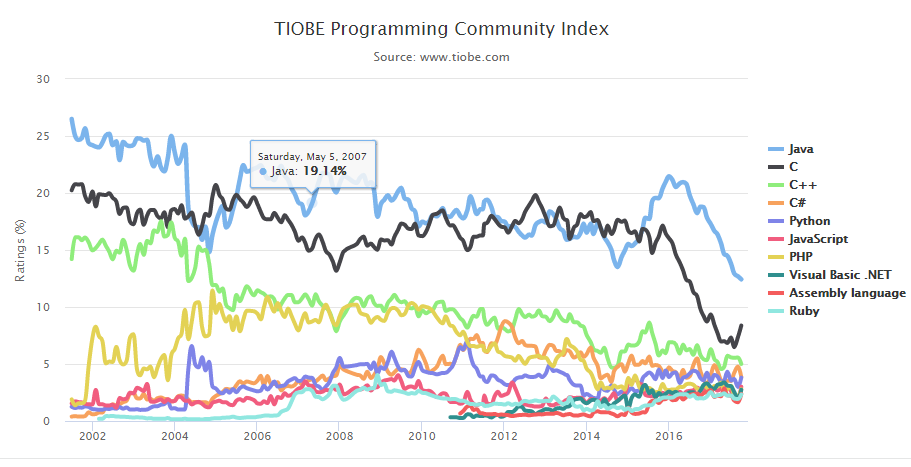
\includegraphics[width=0.7\textwidth]{Java_statics.png}
	\caption{Java statistics}
	\label{JavaStatics}
    \end{figure}
	\begin{figure}[!h]
	\centering
	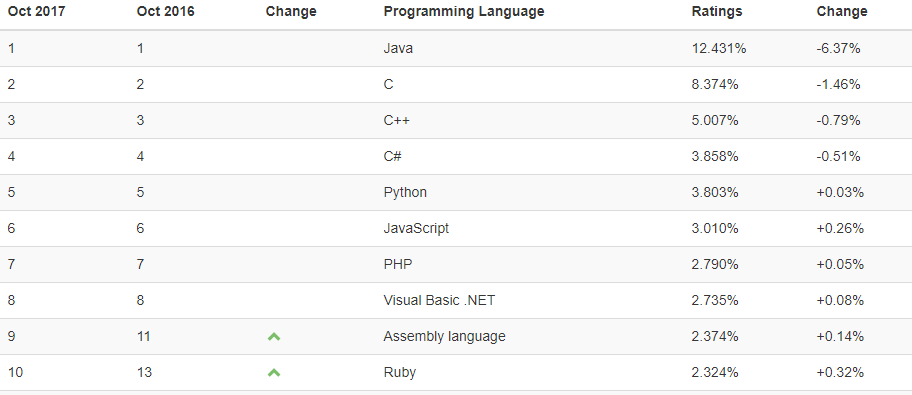
\includegraphics[width=0.7\textwidth]{Java_rank.png}
	\caption{Java rank}
	\label{JavaRank}
    \end{figure}
 
 
\clearpage
\newpage

	\section{Angular JS}
		\begin{figure}[h]
		\centering
		
\includegraphics[width=0.3\textwidth]{AngularJS_logo.png}
		\caption{AngularJS}
	\end{figure}
		\subsection{Definition}
	AngularJS is a structural framework for dynamic web applications.
	\\
	\\
	It gives to the developers the way to interacte with their html components in ease way instead of using a long javascript code.
	\\
	\\
	The impedance mismatch between dynamic applications and static documents is often solved with \cite{ref8} :
	\begin{itemize}
		
		\item \textbf{a library} - a collection of functions which are useful when writing web apps. Your code is in charge and it calls into the library when it sees fit. E.g., \colorbox{mygray}{jQuery}.
		\item \textbf{frameworks} - a particular implementation of a web application, where your code fills in the details. The framework is in charge and it calls into your code when it needs something application specific. E.g., \colorbox{mygray}{durandal}, \colorbox{mygray}{ember}, etc.
	\end{itemize}
	AngularJS takes another approach. It attempts to minimize the impedance mismatch between document centric HTML and what an application needs by creating new HTML constructs. AngularJS teaches the browser new syntax through \textbf{directives}. Examples include:
	\begin{itemize}
		\item Data binding, as in \colorbox{mygray}{\{\{\}\}}
		\item DOM control structures for repeating, showing and hiding DOM fragments.
		\item Support for forms and form validation.
		\item Attaching new behavior to DOM elements, such as DOM event handling.
		\item Grouping of HTML into reusable components.	
	\end{itemize}
	\subsection{Features}
	\begin{itemize}
		\item AngularJS is a powerful JavaScript based development framework to create Rich Internet Application(RIA).
		\item AngularJS is a free open source framework.
		\item Large of developers around the world used AngularJS
	\end{itemize}
		Overall, AngularJS is a framework to build large scale and high performance web application while keeping them as easy-to-maintain.
		\\
		\\
The Table. \ref{DUOP} presented the list of AngularJS directives used.
		\begin{table}[!b]
				\caption{\textbf{Directives used in our project }.}
			\label{DUOP}
				\centering
			\begin{tabular}{|c|p{10cm}|}	
				\hline
				\textbf{Directive} & \textbf{Description }\\
				\hline
				ng-app & tells AngularJS that this is the root element of AngularJS application, we can only have one ng-app directive in the application.
				\\
				\hline
				ng-model & binds an HTML form element to a variable in the scope  \\
				\hline
				ng-switch, ng-switch-when & the directive ng-switch lets you hide or show HTML elements depending on an expression. Child elements with the directive ng-switch-when will be showed up if it gets match, otherwise the element, and its children will be removed.
				\\
				\hline
				ng-switch-default & define a default section if none of the oher sections get match\\ 
					
				\hline
			\end{tabular} 
		\end{table}
	
	\subsection{Motivation}
	Before starting to use any javascript framework, we have made a research about the most recommended javascript framework.
	\\
	Almost all the articles that I read shows that the most popular frameworks are \colorbox{mygray}{AngularJS}, \colorbox{mygray}{Ember.js}, \colorbox{mygray}{ReactJS} and \colorbox{mygray}{Backbone.js}, AngularJS is the most used framework amongst these frameworks and this is my first motivation.\\
    Based on recent search on Google Trends as shown in Fig.\ref{AngularJSOnGoogleTrends}, the requirements skills  of the industry in all over the world tend  to use more and more the framework AngularJS.
	 	\begin{figure}[h]
	 	\centering
	 	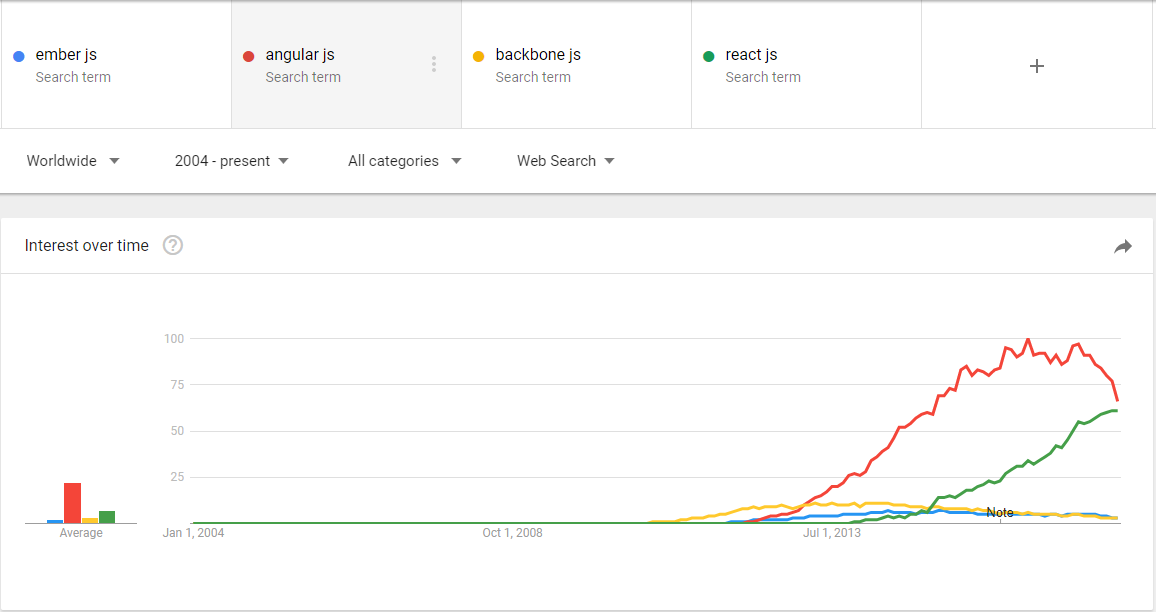
\includegraphics[width=1.0\textwidth]{AngularJS_statics_google_trends.png}
	 	\caption{AngularJS on Google trends}
	 	\label{AngularJSOnGoogleTrends}
	 \end{figure}
	 

\clearpage
\newpage

	\section{Bootstrap}
	\begin{figure}[h]
		\centering
		
\includegraphics[width=0.20\textwidth]{Boostrap_logo.png}
		\caption{Bootstrap}
	\end{figure}
	\subsection{Definition}
	\textbf{Bootstrap} is a free and open-source front-end web framework for designing websites and web applications. It contains HTML- and CSS-based design templates for typography, forms, buttons, navigation and other interface components, as well as optional JavaScript plugins. Unlike many web frameworks, it considers front-end development \cite{ref9}.
	\\
	\\
	Bootstrap was developed by Mark Otto and Jacob Thornton at Twitter, and released as an open source product in August 2011 on GitHub.\\
	In June 2014 Bootstrap was the No.1 project on GitHub!
	\subsection{Features}
	\textbf{Bootstrap 3} supports the latest versions of the \textbf{Google Chrome}, \textbf{Firefox}, \textbf{Internet Explorer}, \textbf{Opera}, and \textbf{Safari} (except on Windows). It additionally supports IE8 and the latest Firefox Extended Support Release (ESR).
	\\
	Since \textbf{2.0}, \textbf{Bootstrap} supports \textbf{responsive web design}. This means the layout of web pages adjusts dynamically, taking into account the characteristics of used device (desktop, tablet, mobile phone).
	\\
	Starting with \textbf{version 3.0}, Bootstrap adopted a mobile-first design philosophy, emphasizing responsive design by default.The \textbf{version 4.0} alpha release added \textbf{Sass} and \textbf{flexbox} support.
	\subsection{Motivation}
	All the research shows that Bootstrap is The most popular HTML, CSS, and JavaScript framework for developing responsive, mobile first projects  on the web.\\According to github, Bootstrap is the second starred repository, with \textbf{115k stars} as shown in Fig. \ref{BootstrapSecondStarredOnGitHub}.
	According to a research in the net, all the high-tech blogs encourage developers to use bootstrap.
		\begin{figure}[h]
		\centering
		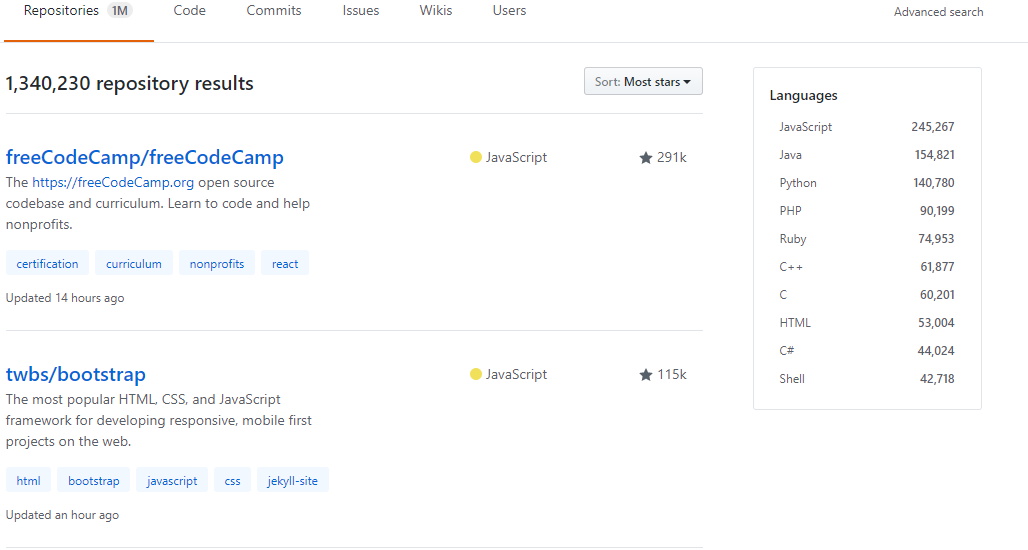
\includegraphics[width=15.5cm,height=9cm]{Boostrap_statics_github.png}
		\caption{Bootstrap second starred on GitHub}
		\label{BootstrapSecondStarredOnGitHub}
	\end{figure}
\\
 I used a tool offred by Google named \textbf{Google trends} to make a compraison between subjects in term of most researched.
 \\
 After this compraison in Google trends, Bootstrap also is the most googled css framework on the web as shown in Fig. \ref{BootstrapOnGoogleTrends} , compared to the others css frameworks Eg. \textbf{Material UI} which was considered as the most popular css framework after Bootstrap.

\begin{figure}[!h]
	\centering
	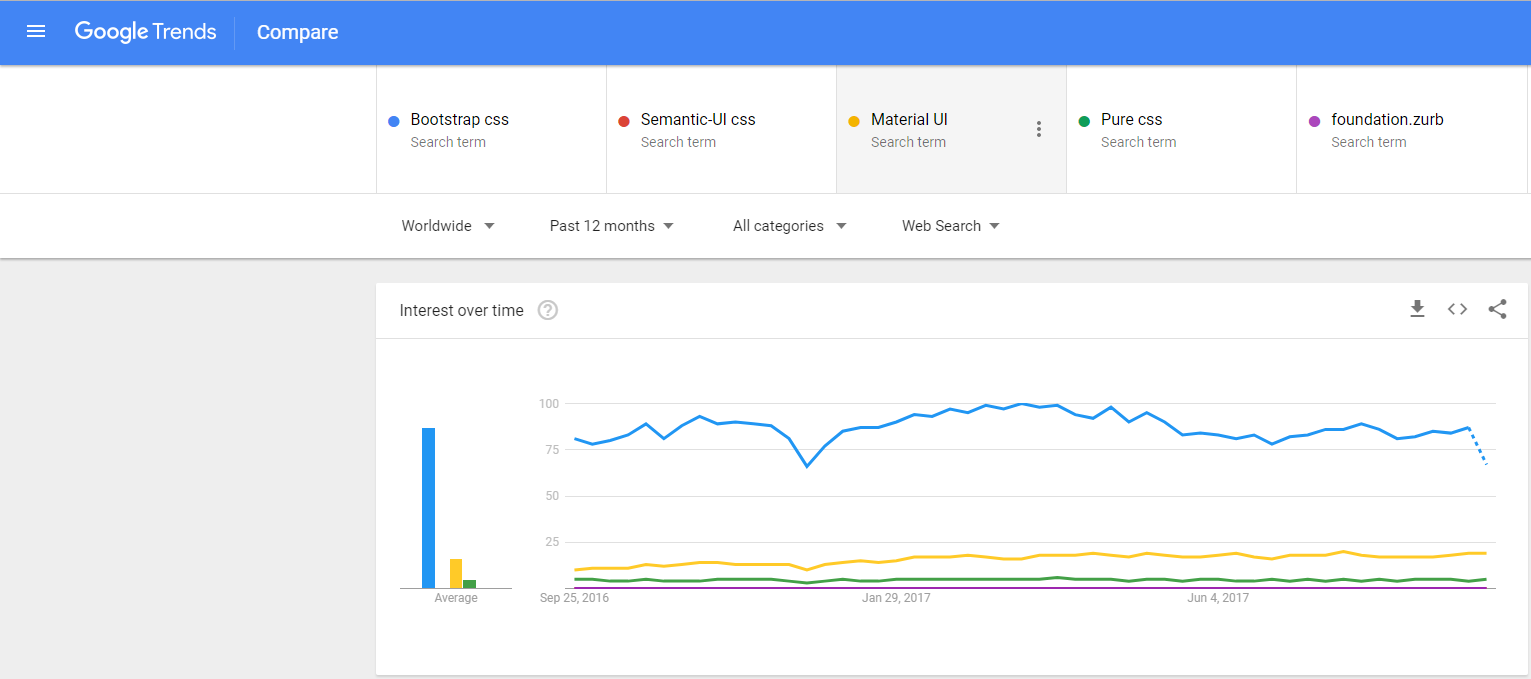
\includegraphics[width=15.5cm,height=9cm]{Boostrap_statics_google_trends.png}
	\caption{Bootstrap on Google trends}
	\label{BootstrapOnGoogleTrends}
\end{figure}

\section{Spring MVC framework}

\subsection{Definition}

The Spring Web model-view-controller (MVC) framework is designed around a \colorbox{mygray}{DispatcherServlet} that dispatches requests to handlers, with configurable handler mappings, view resolution, locale, time zone and theme resolution as well as support for uploading files. The default handler is based on the \colorbox{mygray}{@Controller} and \colorbox{mygray}{@RequestMapping} annotations, offering a wide range of flexible handling methods. With the introduction of Spring 3.0, the \colorbox{mygray}{@Controller} mechanism also allows you to create RESTful Web sites and applications, through the \colorbox{mygray}{@PathVariable} annotation and other features.
\begin{figure}[!b]
	\centering
	
\includegraphics[width=0.2\textwidth]{Spring_logo.png}
	\caption{Spring MVC}
\end{figure}
Spring’s web MVC framework is, like many other web MVC frameworks, request-driven, designed around a central Servlet that dispatches requests to controllers and offers other functionality that facilitates the development of web applications. Spring’s DispatcherServlet however, does more than just that. It is completely integrated with the Spring IoC container and allows you to use every other feature that Spring has. The request processing workflow of the Spring Web MVC DispatcherServlet is illustrated in the Fig. \ref{WorkflowSpringMVC} . The pattern-savvy reader will recognize that the DispatcherServlet is an expression of the ``Front Controller'' design pattern (this is a pattern that Spring Web MVC shares with many other leading web frameworks).
\begin{figure}[!h]
	\centering
	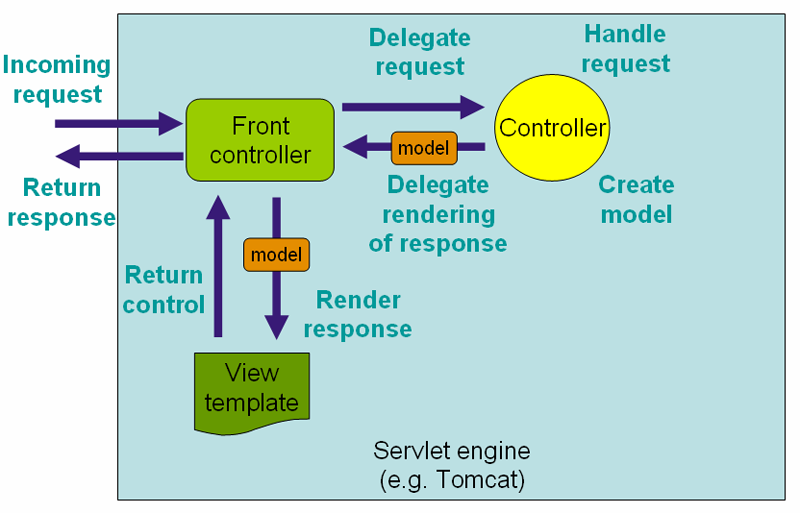
\includegraphics[width=15.5cm,height=10cm]{workflow_spring_mvc.png}
	\caption[The request processing workflow in Spring Web MVC]{The request processing workflow in Spring Web MVC \cite{ref10}}
	\label{WorkflowSpringMVC}
\end{figure}


\subsection{Features}
\begin{itemize}
	\item Since Spring MVC framework is designed like any other Spring module, So, it is not necessary to spend any extra time to learn it.
	\item Since all the layers are independent of each others, unit testing can be easier.
	\item Spring framework doesn’t force you to follow any pattern, or implementations to write your business logic. So it gives developer flexibility to implement or integrate any other design pattern to suffice his needs.
	\item Spring provides good separation flexibility between Controller, Service and Data access layers.
	\item Spring provides you with a tag library that is simple and yet very powerful.
	\item View side you can integrate with any UI framework like JSF, Velocity, Freemarker etc.
	\item Supports Annotation based programming along with XML, which makes development faster and cleaner.
\end{itemize}
The Table. \ref{TabAU} presented the list of spring mvc annotation used to develop our project.
\begin{table}[h]
	\caption{ \textbf{Annotations used in our project}}
	\label{TabAU}
	\centering
	\begin{tabular}{|c|p{10cm}|}
		\hline
		\textbf{Annotation} & \textbf{Description }\\
		\hline
		@Controller & it is responsible for preparing a model Map with data and selecting a view name but it can also write directly to the response stream and complete the request.  \\
		\hline
		@RequestMapping & it used with method to provide the URI pattern for which handler method will be used.\\
		\hline
		@RequestBody & the @RequestBody method parameter annotation indicates that a method parameter should be bound to the value of the http request body.  \\
		\hline
		@ResponseBody & it used to send String response for the web request.  \\
		\hline	
		@RequestParam & it used to retrieve the URL parameter and map it to the method argument. \\
		\hline
	\end{tabular}
\end{table}


\subsection{Motivation}
According to trusted sources like google engine, yahoo, Linkedin and satckoverflow: spring mvc, struts And JSF are the most JEE frameworks searched and posted by the developers.\\
\begin{figure}[!h]

	\centering
	\includegraphics[width=0.8\textwidth]{SpringMVC_statics_google_trends.png}
	\caption{Spring framework on google trends}
	\label{SpringMVC_statics_google_trends}
\end{figure}
\\
The curve of spring mvc as shown in the Fig. \ref{SpringMVC_statics_google_trends} is very high, wich means that spring is the most used among others frameworks, another key is That spring is the most framework recommend on job application.
\\
\\
The community behind spring is very active.

\section{Pivotal tc Server}

\begin{figure}[!h]
	
	\centering
	
\includegraphics[width=0.1\textwidth]{icon_tcserver.png}
	\caption{Pivotal tc Server}
	\label{Pivotal tc Server}
\end{figure}

Pivotal tc Server is a open-source Web application server based on Apache Tomcat \cite{ref11} .
\\
\\
Pivotal tc Server provides :
\begin{itemize}
	\item The best of Apache Tomcat.
	\item Harnesses the power of traditional JEE architectures.
	\item Eliminates the JEE's complexity and performance drawbacks, making it easier, faster.
	\item Pivotal tc Server requires significantly fewer resources than conventional servers.
	\item It is completely compatible with Apache Tomcat.
\end{itemize}



\section{Spring Tool Suite}

\begin{figure}[!h]
	
	\centering
	
\includegraphics[width=0.1\textwidth]{spring-tool-suite-project-logo.png}
	\caption{Spring tool suite}
	\label{spring tool suite}
\end{figure}
\begin{itemize}
	\item The Spring Tool suite is an eclipse-based developing environment that customized for development  Spring applications.
	\item Provides a environment to implement, debug, run, and deploy.
	\item It integrates Git,Maven, Pivotal tc Server but also you can use other Web Application Server. 
\end{itemize}


\section{Apache Maven}
\begin{figure}[!h]
	\centering
	
\includegraphics[width=0.1\textwidth]{Maven_logo.png}
	\caption{Apache Maven}
\end{figure}
Maven is an open-source tool developed by the foundation Apache, which main role is to build projects and the management of libraries used \cite{ref12}
\\
\\
Maven provides :
\begin{itemize}
	\item compilation
	\item packaging
	\item dependency management
	\item deployment
\end{itemize} 

\section{HTML5}
\begin{figure}[!h]
	\centering
	
\includegraphics[width=0.1\textwidth]{HTML5_logo.png}
	\caption{HTML5}
\end{figure}
HTML5 is the last version of HTML, it comes with new semantics tags (header,aside,...) to divide your page in semantic way, those tags it helps the engine (Google, yahoo...) to perform the results. It is easy to learn, compatible with all browsers, now HTML5 replace the falsh, it include tag video, audio, Geo-localization, and more \cite{ref13}.
\section{Web Service}
\subsection{Definition}
\subsection{SOAP}
	SOAP (Simple Object Access Protocol) is a messaging protocol that allows the different parts of your application to run on disparate platform, in our case the API MassTerServer running on Windows Server AWS EC2 communicate with MassTerInsight (running on AWS EB) using SOAP Protocol.
	MassTer Server API publish his service using SOAP web service.   
\subsection{REST}
	REST (REprensentation state transfer) web service it is a way of providing interoperability between different platform and programming language on the internet.
	In our case we use REST API to communicate between the framework AngularJS (javascript) and the framework spring mvc (java). 
\section{Cloudforge}
\subsection{Definition}   
\begin{figure}[h]
	\centering
	\includegraphics[width=0.2\textwidth]{logocloudforge.png}
	\caption{Cloudforge}
\end{figure}
CloudForge is a new development Platform as a Service (dPaaS) for developing, deploying and scaling application services. CloudForge marries collaborative application development with a simplified approach for deploying to PaaS and any production server \cite{ref13} it allows the user to :
 
 \begin{itemize}
 	\item manage and integrate your development tools.
 	\item elastically scale your teams, projects and processes.
 	\item deploy your code to public and private Cloud.
 \end{itemize}
Cloudforge makes the job of each member in the team more efficient, by gives for each other a set of features.
\\
\\
For \textbf{Managers}, it allows them to : 
\begin{itemize}
	\item easily manage the team members
	\item be the medium between different teams
	\item planning Releases and Sprints
	\item improve the process of development retrospective ideas
\end{itemize} 
For \textbf{Product owner}, it allows them to :
\begin{itemize}
	\item have an instant feedback of the newly-made changes;
	\item easily plan the characteristics of the product;
	\item directly connect to developers;
    \item  define the timeline for the projects (releases, demos, sprints).
\end{itemize}
For \textbf{Developers}, it allows them to:
\begin{itemize}
	\item follow up with the work;
	\item easily identify the status of a sprint;
	\item consult the last task one must do in the backlog
\end{itemize}

\subsection{Team presentation}
MASS Analytics relies heavily in almost every layer of its business and project management. It allows the company to handle changing requirements in an efficient way and to follow the footsteps of grand leading organizations in software development.
Scrum methodology is based on four pillars as presented in the Table \ref{RTM}.

 \begin{table}[!h]
	\caption{\textbf{Roles of the team members}.}
	\label{RTM}
	\centering
	
	\begin{tabular}{|c|p{8cm}|p{5cm}|}
		\hline 	
		\textbf{Role } & \textbf{Mission } & \textbf{Team Member }  \\ 
		\hline                     
		\textbf{Developer} & To implement the features of MassTer Insight and deployed in the cloud & Radhouan Hrizi \\
		\hline 
		\textbf{Scrum Master} & To assign tasks and to test the implemented features, report bugs if found, implement new features in massTer Server API & Amira Ben Mansour \\
		\hline 
		\textbf{Product Owner} & To plan meeting, validate the new features. & Firas Jabloun \\  
		\hline 
		
	\end{tabular}
\end{table}


\section{Deployment}

\subsection{Definition}
In this final section we will discuss the phase of deployment, we used the amazon web service to deploy our web application and MassTer Server API.
\subsection{Amazon Web Services}
\begin{figure}[!h]
	\centering
	
\includegraphics[width=0.2\textwidth]{aws-logo.png}
	\caption[Amazon Web Services]{Amazon Web Services \cite{ref14}}
\end{figure}
\subsubsection{Introduction}
Amazon Web Service is Cloud computing Platform provided by Amazon.com. The first AWS were launched in 2006 to provide online services fo websites and client-side applications.

\subsubsection{Elastic Beanstalk}
Amazon Elastic Beanstalk is cloud deployment and provisioning service that automates the process of getting application set up on the Amazon Web Services (AWS) infrastructure. To use the service, developers just have to upload their applications. Elastic Beanstalk support application written in Java, Node.JS, PHP, Python, Ruby, and .Net.
\\
\\
After packaging our Web Application to .WAR using Apache MAVEN, then we deployed this package in Elastic beanstalk, the platform were the application is running is Tomcat as shown in Fig. \ref{ElasticBeanstalkApplication} and Fig. \ref{massTerInsightDashboard}.

\begin{figure}[!h]
	\centering
	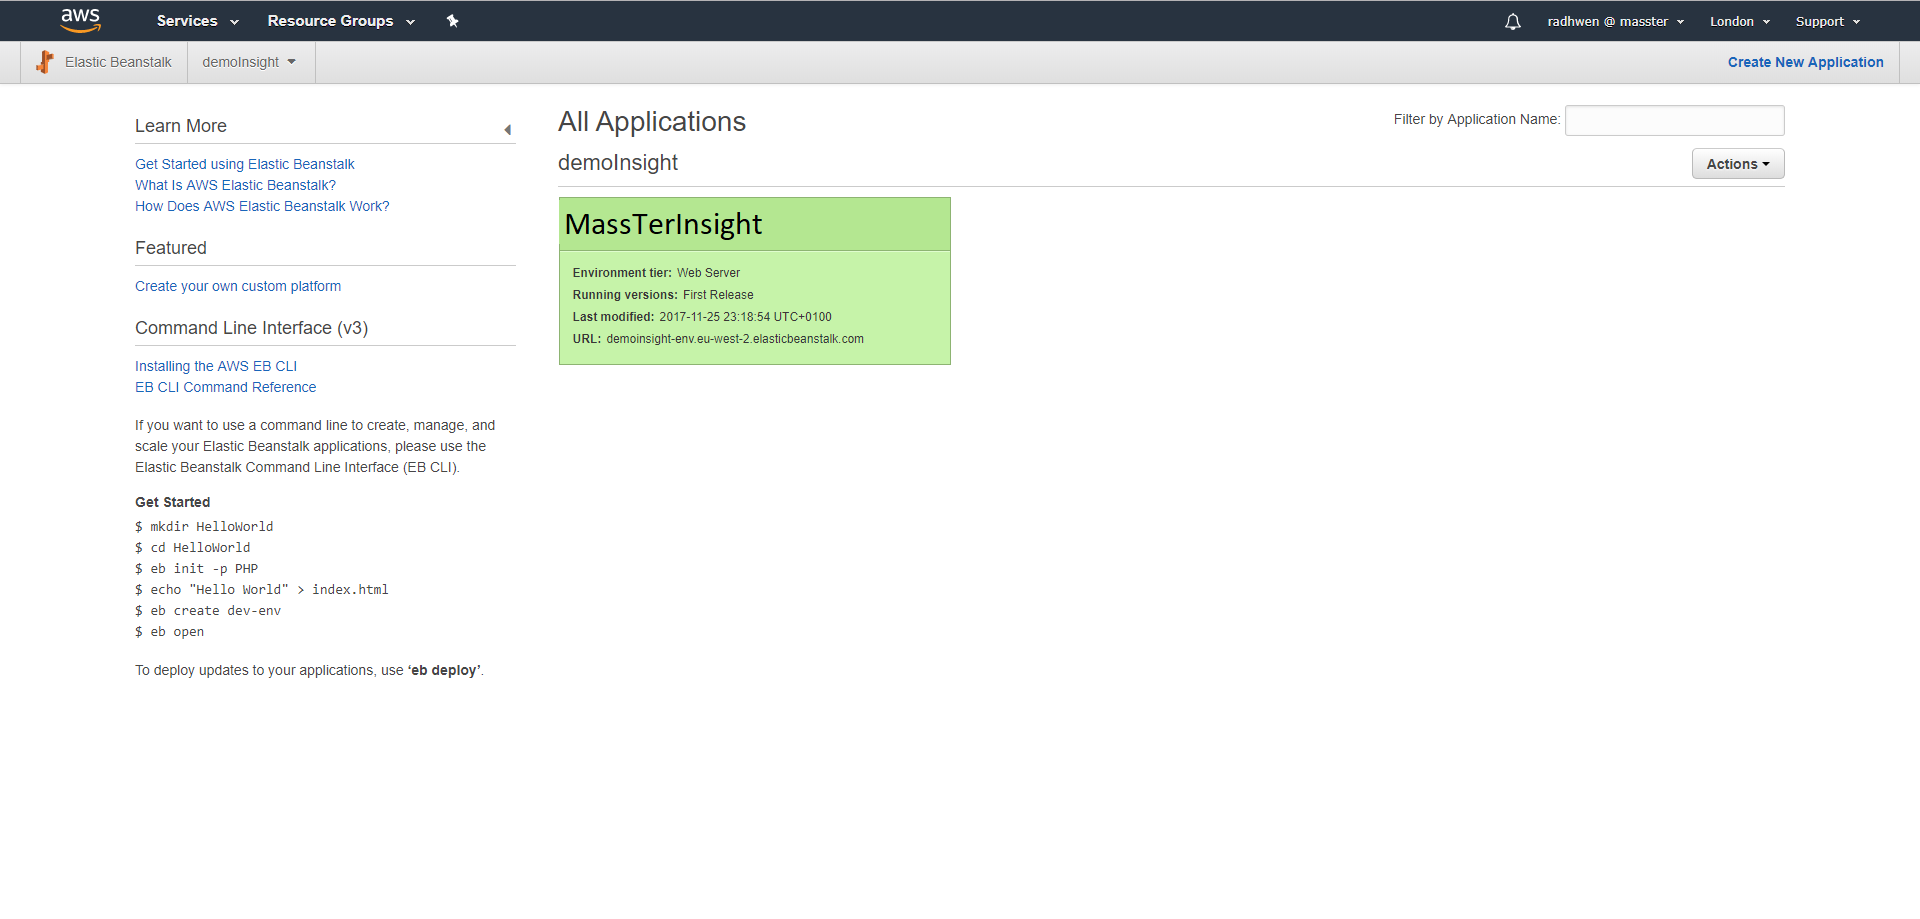
\includegraphics[width=17cm,height=7cm]{ElasticBeanstalkApplication.png}
	\caption{Elastic Beanstalk Application}
	\label{ElasticBeanstalkApplication}
\end{figure}

\clearpage
\newpage 
\begin{figure}[!h]
	\centering
	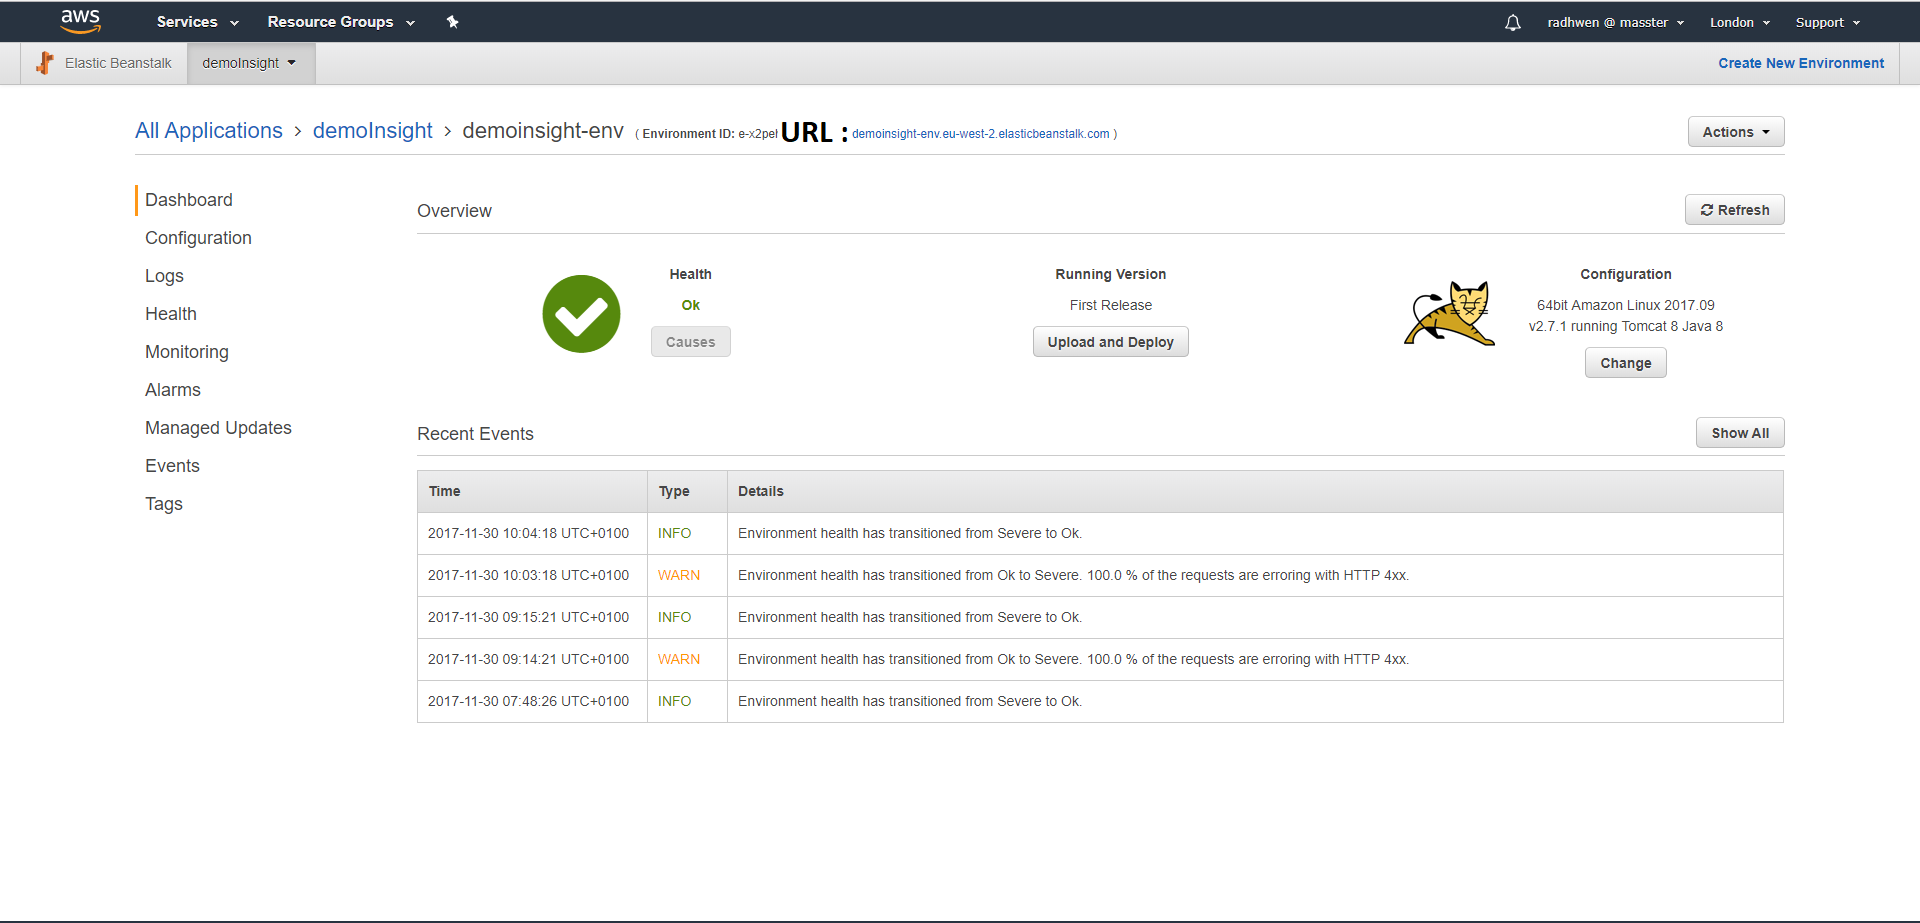
\includegraphics[width=17cm,height=7cm]{massTerInsightDashboard.png}
	\caption{MassTer Insight web Application Dashboard}
	\label{massTerInsightDashboard}	
\end{figure}

After the deployment is done successfully, elastic beanstalk provides a URL for our application to be accessible in the INTERNET as presented in the Fig. \ref{MassTerInsightwebApplication}.
\begin{figure}[!b]
	\centering
	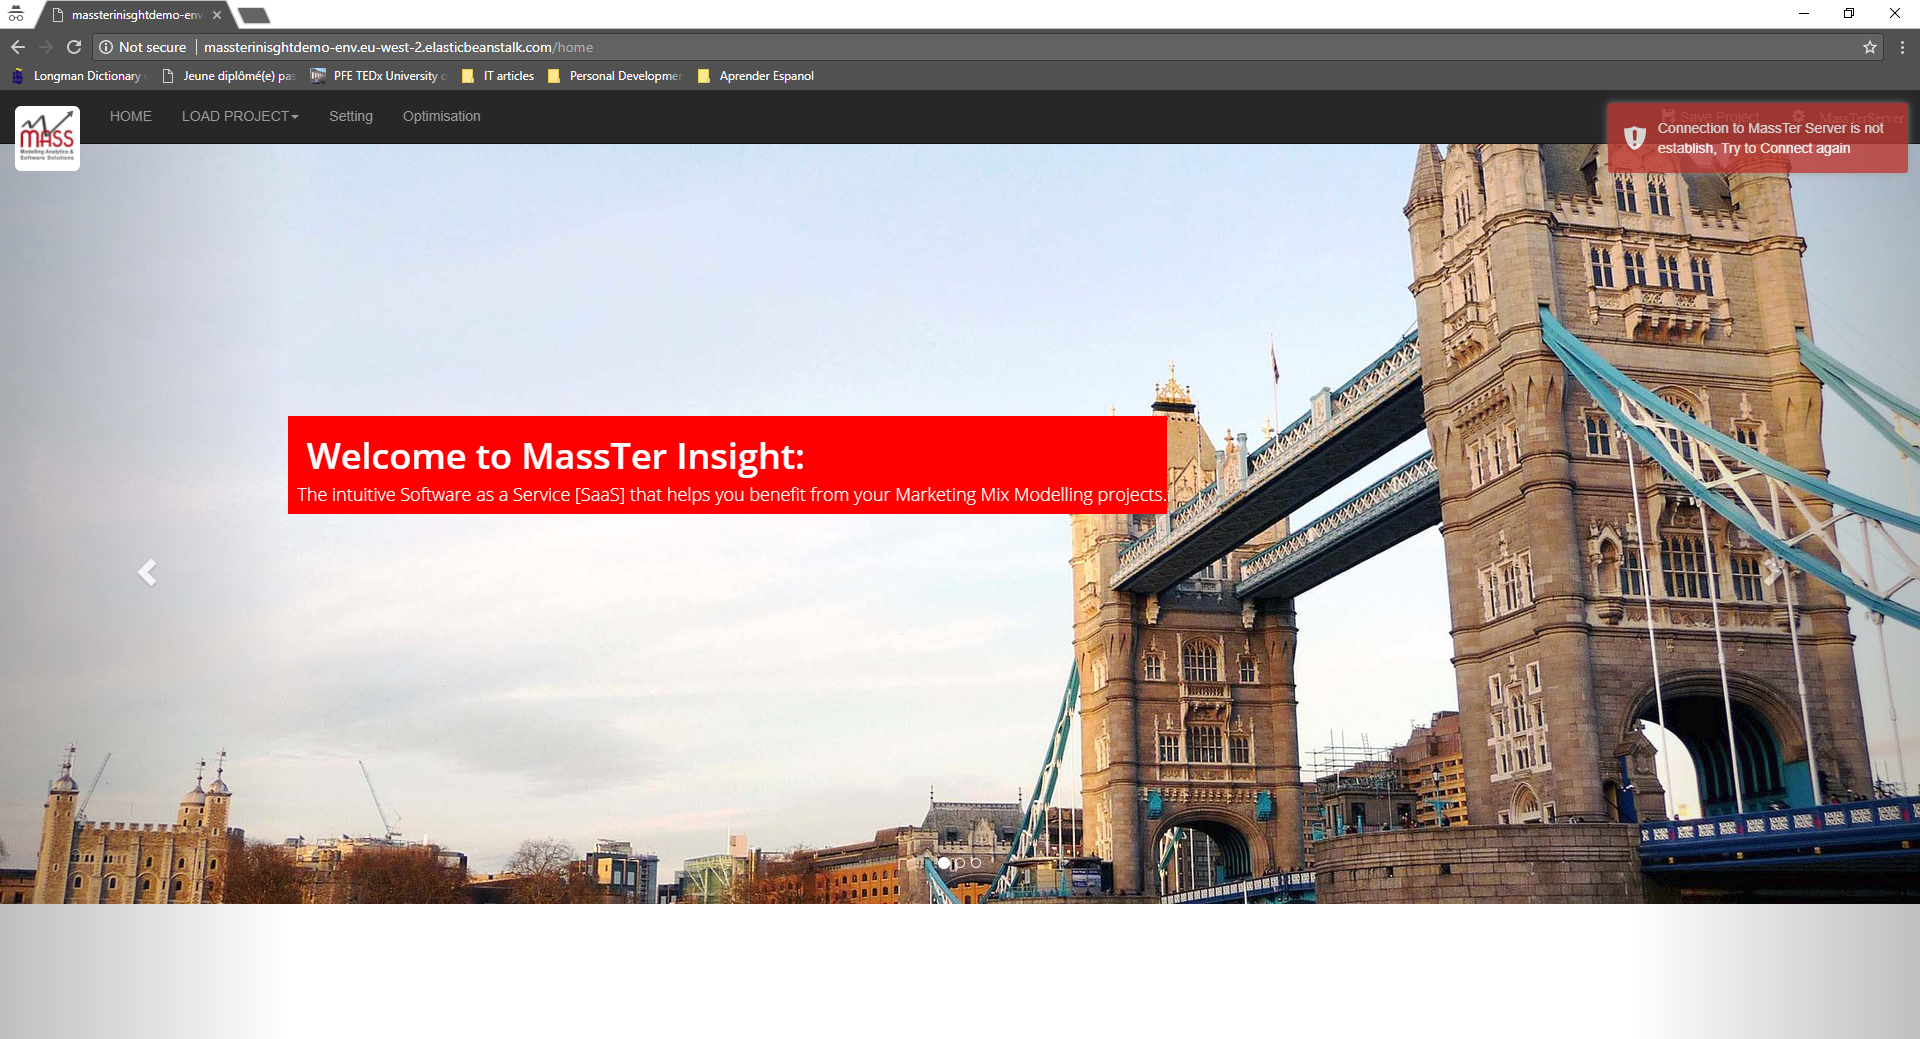
\includegraphics[width=17cm,height=7cm]{1.png}
	\caption{MassTer Insight web Application}
	\label{MassTerInsightwebApplication}	
\end{figure} 
\clearpage
\newpage 
Fig. \ref{CMSAscreentshots} shows the interface for the connection to the MassTer Server API. In which we should type the IP address and the port number  to access to the server.
\begin{figure}[!h]
	\centering
	
	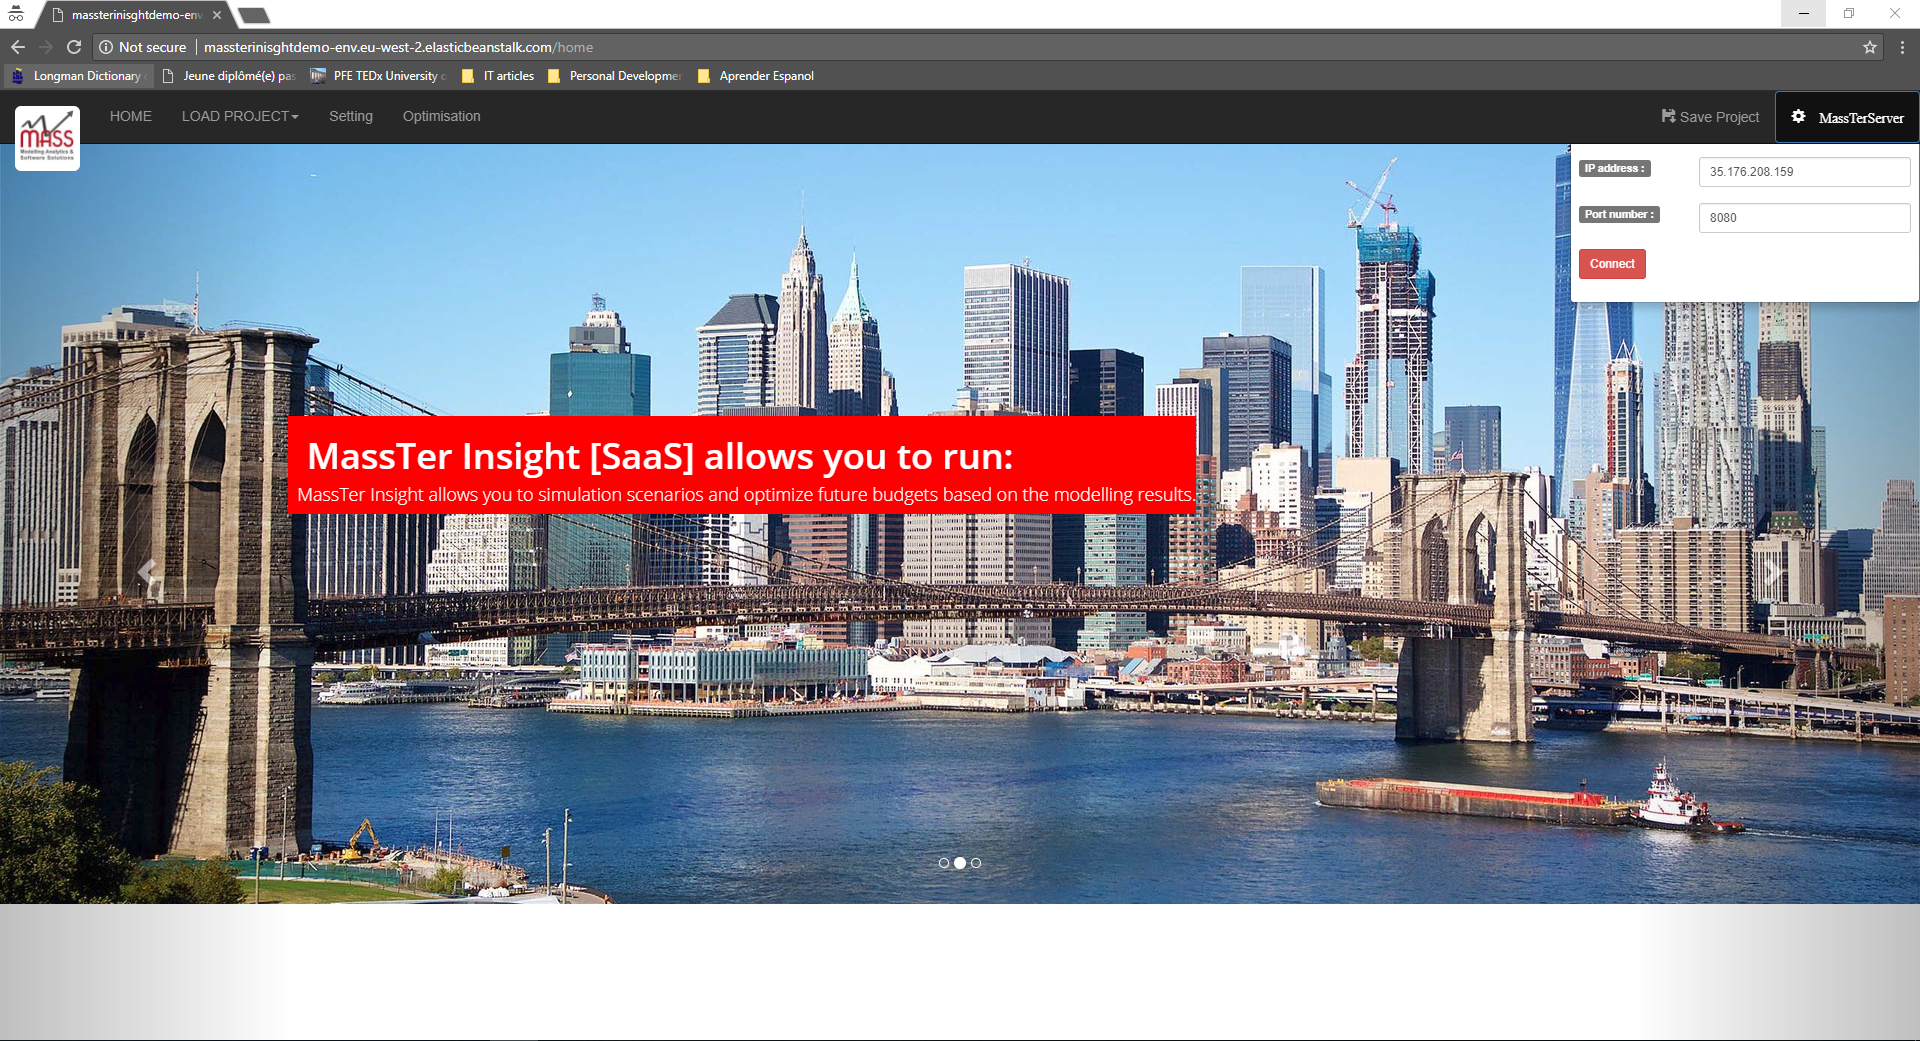
\includegraphics[width=17cm,height=7cm]{2.png}
	\caption{Connect to MassTer Server API}
	\label{CMSAscreentshots}
\end{figure}

Fig. \ref{LMIPscreentshots} shows the interface for load MassTer insight project by typing the name of the project in the text-field. 
\begin{figure}[!h]
	\centering
	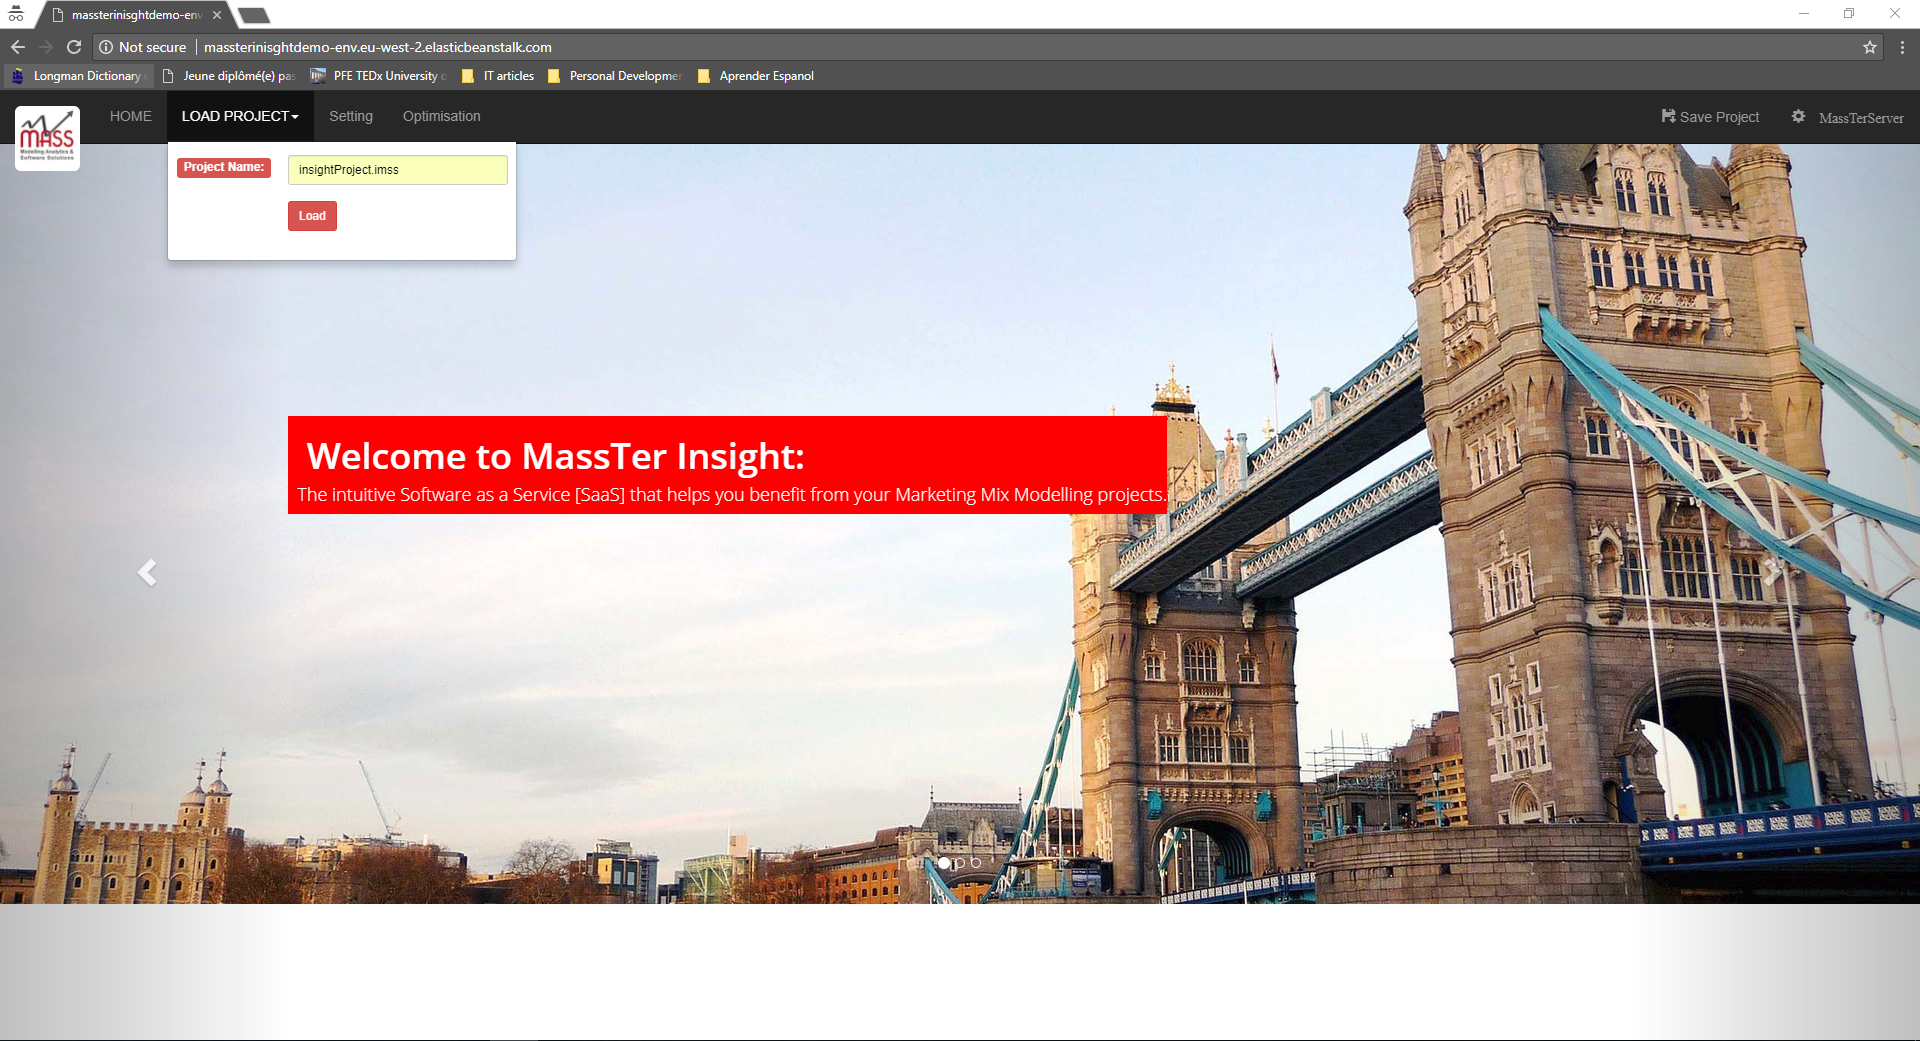
\includegraphics[width=17cm,height=7cm]{3.png}
	\caption{Load MassTer Insight Project}	
	\label{LMIPscreentshots}
\end{figure} 
\clearpage
\newpage 
Fig. \ref{DORscreentshots} shows the information related to the selected report ``Monthly 150''.
\begin{figure}[!h]
	\centering
	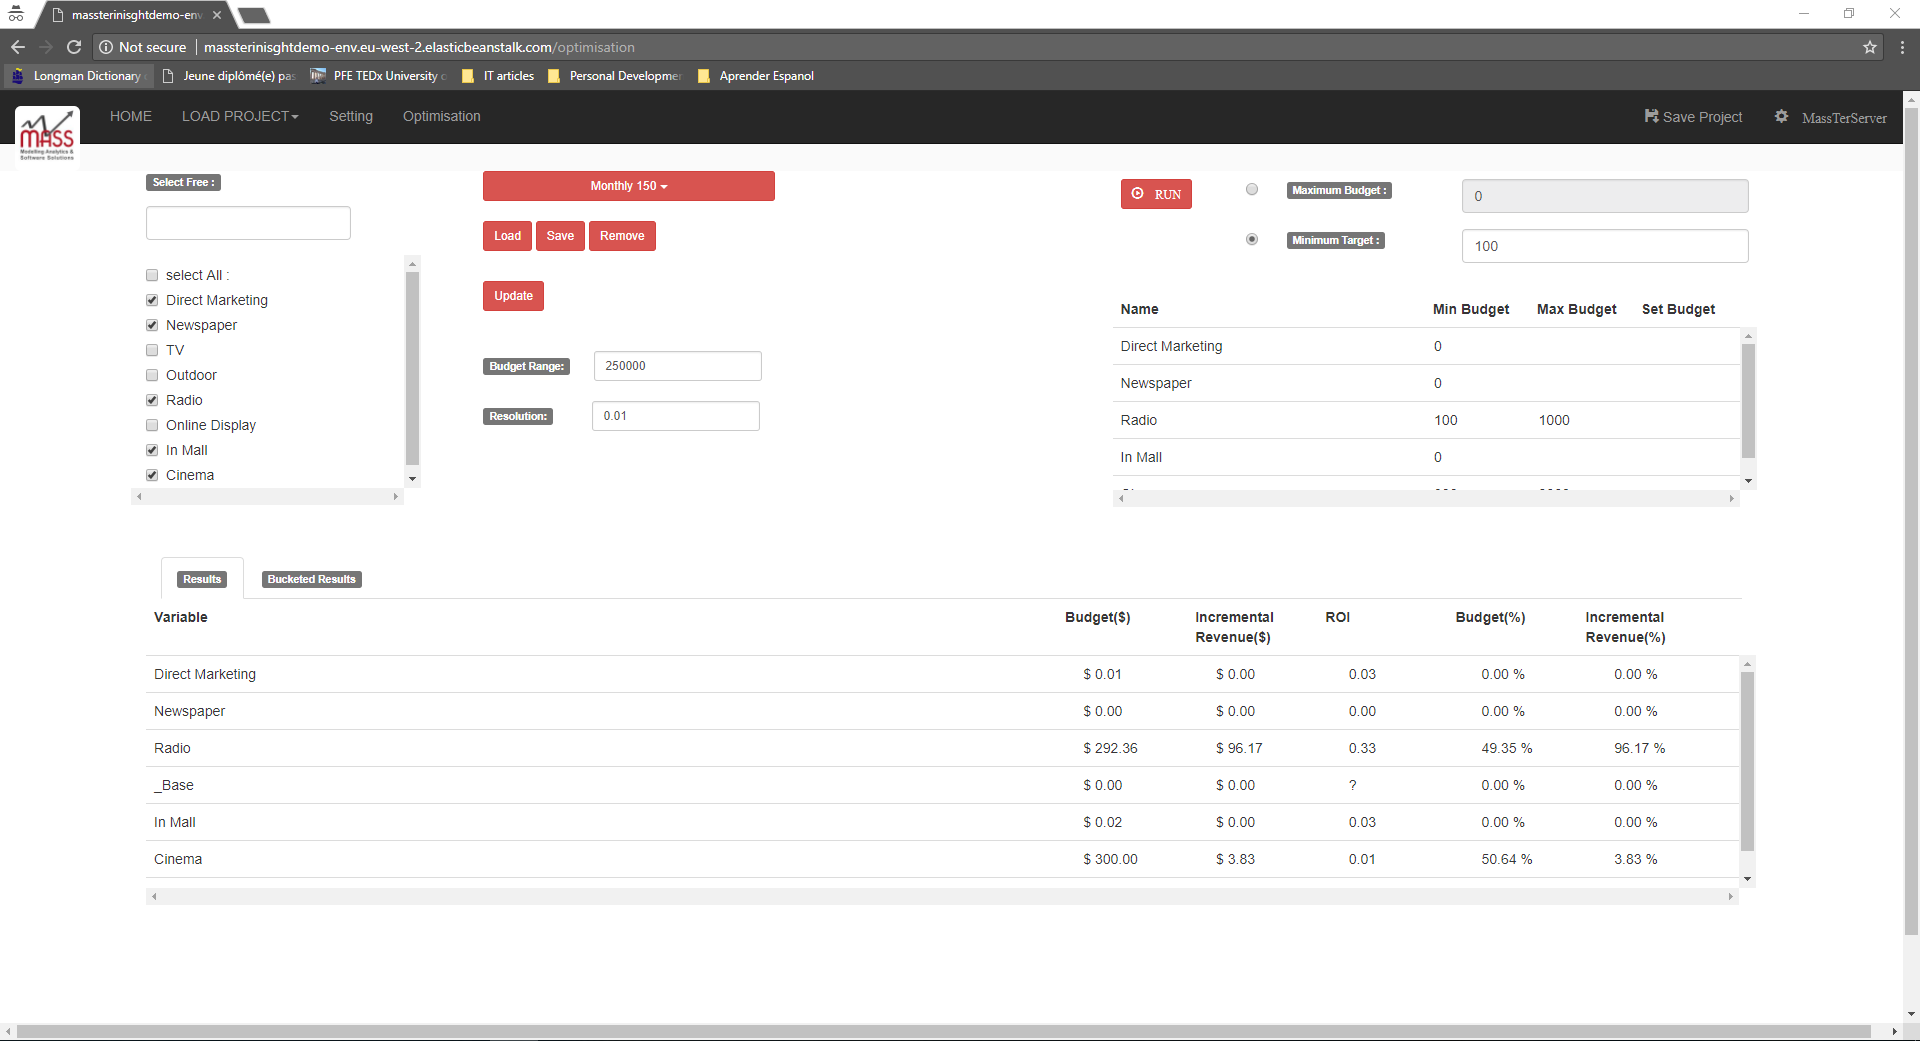
\includegraphics[width=17cm,height=7cm]{4.png}
	\caption{Display Optimisation Report}
	\label{DORscreentshots}	
\end{figure}

Fig. \ref{LARscreentshots} shows the list of the existing reports (Monthly 150, Monthly 250, Monthly 300, Monthly 400, Monthly 200, monthly amira) in the project ``insightProject.imss''.
\begin{figure}[!h]
	\centering
	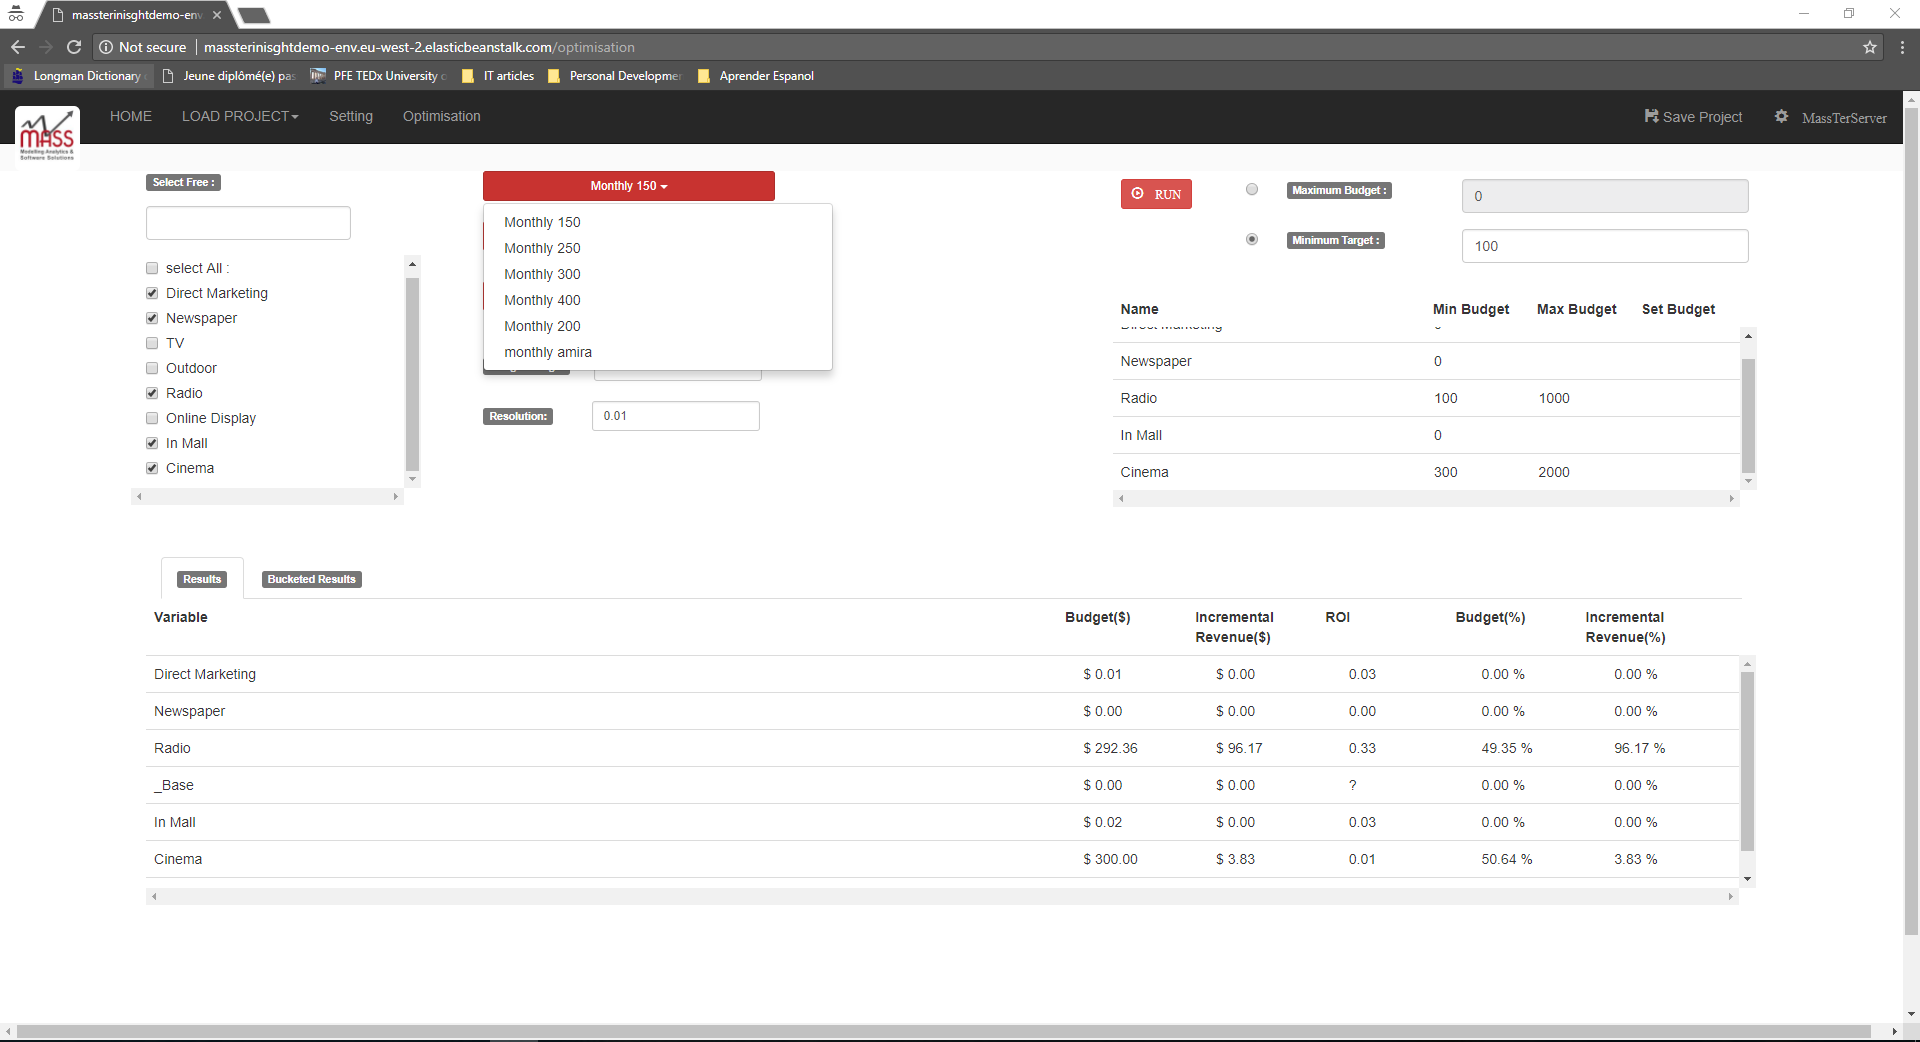
\includegraphics[width=17cm,height=7cm]{5.png}
	\caption{List Available Reports}
	\label{LARscreentshots}	
\end{figure} 
\clearpage
\newpage 
Fig. \ref{UDWSscreentshots} shows that the update is done with success after choosing  TV and Radio as channels.
\begin{figure}[!h]
	\centering
	\includegraphics[width=17cm,height=7cm]{6.png}
	\caption{Update done with Success}
	\label{UDWSscreentshots}	
\end{figure}

Fig. \ref{ROWSscreentshots} shows that Run of a new Optimisation is done with success after choosing Budget Range 250000 \$ and Min-Target 100 \$.    
\begin{figure}[!h]
	\centering
	\includegraphics[width=17cm,height=7cm]{7.png}
	\caption{Run Optimisation with Success }
	\label{ROWSscreentshots}	
\end{figure} 
\clearpage
\newpage 
Fig. \ref{DBMCscreentshots} depicts the allocated budgets for each channel (TV and Radio) in each month.
\begin{figure}[!h]
	\centering
	\includegraphics[width=17cm,height=7cm]{8.png}
	\caption{Display budget per Month for each Channel}
	\label{DBMCscreentshots}
\end{figure}

Fig. \ref{DCMCscreentshots} depicts the incremental revenue for each channel (TV and Radio) in each month.
\begin{figure}[!h]
	\centering
	\includegraphics[width=17cm,height=7cm]{9.png}
	\caption{Display Contribution per Month for each Channel}
	\label{DCMCscreentshots}	
\end{figure} 
\clearpage
\newpage 
Fig. \ref{SPscreentshots} displays the drop down save project (save/save as).
\begin{figure}[!h]
	\centering
	\includegraphics[width=17cm,height=7cm]{10.png}
	\caption{Save Project}
	\label{SPscreentshots}	
\end{figure}

Fig. \ref{SPWSscreentshots} shows  a blue pop up information to inform the user that the project is saved with success after click on the item ``save'' in drop down save project.
\begin{figure}[!h]
	\centering
	\includegraphics[width=17cm,height=7cm]{11.png}
	\caption{Save Project with Success}
	\label{SPWSscreentshots}		
\end{figure} 
\clearpage
\newpage 

\subsubsection{Elastic Compute Cloud}
Amazon EC2 is an \textbf{IaaS} offering from AWS. Amazon takes the responsibility of networking, storage, server and virtualization and the user is responsible for managing the operating System, middleware, runtime, data and application.


\begin{figure}[!h]
	\centering
	\includegraphics[width=17cm,height=9cm]{ec2Instance.png}
	\caption{EC2 Instance}
	\label{EC2Instance}	
\end{figure} 

MassTer Server API is running on EC2 Instance as shown in Fig. \ref{EC2Instance}, we have chosen Windows Server 2016 as operating System, RAM 1Go, 30 Go Storage. 

\subsection{Conclusion}
Throughout this chapter we described in details the list of technologies that we used to develop this project, we used the highest technologies in web development. Also we present the way we deployed MassTer Server API and MassTer Insight, as a big achievement in this Internship is we  deployed The API MassTer Server and MassTer Insight Web Application successfully Using Amazon Web Services and now our Application Ready to be used through the Internet.


	
       % include chapter 5 %
	\clearpage
	\newpage
	\chapter{Deployment}

	\section{Introduction}
	
	% bibliography  %
	\bibliographystyle{plain}
	\bibliography{webo} 
	
	
\end{document}